%% Šablona pro psaní závěrečných prací FBMI ČVUT
% Upraveno na základě požadavků na závěrečné práce schválených dne 24.2.2020.
%
% Vytvořeno ve spolupráci členů BRAIN Teamu.
% 
% Šablonu pro vás upravil/a:    Ing. Václava Piorecká, Ph.D.
% Kontakt:                      vaclava.piorecka@fbmi.cvut.cz
%
% % % % % % % % % % % % % % % % % % % % % % % % % % % % % % 
%
% 		Upravená verze pro xeLaTeX by Marek Sokol :)			
%  
% % % % % % % % % % % % % % % % % % % % % % % % % % % % % % 

% arara: xelatex: { shell : yes }
%% arara: biber
%% arara: xelatex: { shell : yes }
%% arara: xelatex: { shell : yes }

\documentclass[a4paper,12pt]{article}   % Definice - velikost dokumentu, základní velikost písma, typ
\usepackage[a4paper, top=2.5cm, left=3.5cm, right=2.5cm, bottom=2.5cm]{geometry}		% nastavení okrajů

%% Přidání balíčků podporujících různé funkcionality - ZÁKLADNÍ
\usepackage{amsmath,float}				% balíček pro matiku
\usepackage[dvipsnames]{xcolor}
\usepackage{color}
\usepackage{footnote}					% poznámka pod čarou
\usepackage{url}						% url odkazy
\DeclareUrlCommand\url{\def\UrlLeft{<}\def\UrlRight{>} \urlstyle{same}}   % nastavení URL odkazů pro podle normy ČSN ISO 690

\usepackage{float}						% plovoucí prostředí
%\usepackage[utf8]{inputenc}			% kódování (v tomto případě useless protože používáme unicode engine)
\usepackage[czech]{babel}				% čeština
\usepackage{enumitem}      			    % seznamy 
\usepackage{xevlna}						%
\usepackage{subcaption}					%
\usepackage{pdfpages}					%
\usepackage{amsfonts}      				% množiny Z,R,N dvojitě
\usepackage{amssymb}      				% znaky úhlu a tak
\usepackage{graphicx}					%
\usepackage{textgreek}					%
\usepackage{setspace}					%
\usepackage[justification=centering]{caption}
\usepackage{makecell}
\usepackage{multicol}					% tabulka, slučování sloupců
\usepackage{multirow}                   % tabulka, slučování řádků
\usepackage{fancyhdr}					% záhlaví a zápatí stránky
\usepackage{chngcntr}                   % číslování (číslování rovnic, obrázků dle kapitol)
\usepackage{array}                      % rozšíření práce s tabulkami
\usepackage{helvet}                     % předefinuje \sfdefault to uhv (pro úvodní stránku)
\usepackage[flushleft]{threeparttable}  % prostředí pro tabulky - přidává vysvětlující poznámky pod tabulku

\usepackage{tikz}
\usetikzlibrary{shapes.geometric, arrows, fit}
\tikzstyle{startstop} = [rectangle, minimum width=3cm, minimum height=1cm,text centered, draw=white, fill=white]
\tikzstyle{io} = [trapezium, trapezium left angle=70, trapezium right angle=110, minimum width=3cm, minimum height=1cm, text centered, draw=black, fill=white]
\tikzstyle{process} = [rectangle, minimum width=3cm, minimum height=1cm, text centered, draw=black, fill=white]
\tikzstyle{decision} = [diamond, minimum width=3cm, minimum height=1cm, text centered, draw=black, fill=white]
\tikzstyle{invisible} = [rectangle, text=white]
\tikzstyle{arrow} = [thick,->,>=stealth]

% Následující balíčky řeší citace v dokumentu. 
\usepackage{csquotes}   
\usepackage{expl3}                    
\usepackage[style=iso-numeric]{biblatex}
\addbibresource{biblio.bib}             % zdrojový soubor s citacemi

\usepackage{siunitx}					%
%% Přidání balíčků podporujících různé funkcionality - VOLITELNÉ, DOPLŇKOVÉ
% Existuje celá řada dalších
%\usepackage[]{algorithm2e}				    % balíček pro pseudokód
%\usepackage{ifthen}                        % pro algoritmy if else
%\usepackage{paralist}                      % Rozšířená možnost pro seznamy. Větší škála a možnosti jak seznamy dělat automaticky. 
%\usepackage{courier}
\usepackage{fontspec}                       % nastavení specifických fontů
\setmainfont{Times New Roman}
\setsansfont{Arial}
\setmonofont[Scale=0.9]{Courier New}
%\usepackage{icomma}      				    % není mezera za desetinnou čárkou
% \usepackage[titletoc,title]{appendix}     % automatické vytvoření příloh

%% Přidání speciálních příkazů 
\newcommand{\TextUnderscore}{\rule{.4em}{.4pt}}
\newcommand{\at}{\makeatletter @\makeatother}           % Vytiskne zavináč - \at
\newcommand{\degree}[1][]{\ensuremath{{#1}^\circ}}      % Vytiskne stupeň - \degree
\newcolumntype{C}[1]{>{\centering\let\newline\\\arraybackslash\hspace{0pt}}m{#1}}	% zarovnání v tabulce, vycentrování, potřebuje \usepackage{array}
\addto\captionsczech{\renewcommand{\figurename}{Obr.}}		%

% Zalamování slov na konci věty - napodobení justify jako MS-Word
%\tolerance=1
%\emergencystretch=\maxdimen
%\hyphenpenalty=10000
%\hbadness=10000
%\sloppy

%% Ostatní definice a nastavení
\clubpenalty 10000		% penalizace sirotků, sirotek: poslední řádek odstavce je na nové stránce
\widowpenalty 10000		% penalizace vdov, vdova: první řádek nového odstavce je na konci stránky

\DeclareGraphicsExtensions{.pdf,.png,.jpg}	    % nahrávání obrázků, rozšíření
\graphicspath{{assets/}} 				        % umístění obrázků

\counterwithin{figure}{section}         % číslování obrázků dle sekcí/kapitol
\counterwithin{table}{section}          % číslování tabulek dle sekcí/kapitol
\numberwithin{equation}{section}        % číslování rovnic dle sekcí/kapitol

\setlength{\parskip}{6pt}                   % odsazení mezi odstavci
\setlength{\parindent}{0.75cm}              % odsazení odstavců od okraje
\renewcommand{\baselinestretch}{1.20}	    % řádkování 1,2 - odpovídá pevnému řádkování 17 bodů

\usepackage{tocloft}                    % Nastaví tučné zvýraznění sekcí v obsahu
\renewcommand{\cftsecleader}{\cftdotfill{\cftdotsep}}   % přidá vodící linku do obsahu u sekcí

%% Ostatní neimplementované, pouze návod jak případně doplnit
% Vytvořit seznam použitých algoritmů a přejmenování názvu objektu na Algoritmus.
%\usepackage{listings}
%\usepackage[algosection,vlined,linesnumbered]{algorithm2e}
%\SetAlgorithmName{Algoritmus}{algorithm}{Seznam algoritmů}
%\SetKwInput{KwIn}{Vstup}%
%\SetKwInput{KwOut}{Výstup}%

% // TODO: Turn on referencing
% \usepackage{hyperref}%
   
%% Deklarace názvů - přepsat dle autora
\newcommand{\autor}{Marek Sokol}
\newcommand{\vedouci}{Mgr. Ksenia Sedova, Ph.D.}
\newcommand{\nazev}{Zpracování a analýza záznamu srdeční aktivity}
\newcommand{\nazevENG}{Heart activity record processing and analysis}
\newcommand{\typ}{Bakalářská práce}
\newcommand{\rok}{2021}
% Pro program a obor jsou instrukce zde: http://www.fbmi.cvut.cz/fakulta/uredni-deska 
% Nově akreditované mají pouze studijní programy
\newcommand{\program}{Biomedicínská a klinická technika}
\newcommand{\obor}{Biomedicínský technik}       % u nových akreditací vypustit

%% Vlastní začátek dokumentu
\begin{document}

\pagestyle{empty}

\begin{titlepage}
	\begin{center}
		\begin{figure}[!h]
			\centering
			
\includegraphics[width=0.2\textwidth]{symbol_cvut_konturova_verze}
		\end{figure}
		\textsf{\large{\textbf{ČESKÉ VYSOKÉ UČENÍ TECHNICKÉ V PRAZE}}}\\
		%\vspace{0pt}   		
		{\color{NavyBlue}\makebox[\linewidth]{\rule{\textwidth}{0.4mm}}}
		%{\color{NavyBlue}\hrule }  	    \vspace{6pt}
		\textsf{\normalsize{\textbf{FAKULTA BIOMEDICÍNSKÉHO INŽENÝRSVÍ}}}\\
		\textsf{\textbf{Katedra biomedicínské techniky}}\\

		\vfill

		\textsf{\Large{\textbf{\nazev}}}\\
		\vspace{24pt}
		\textsf{\Large{\textbf{\nazevENG}}}\\
		\vspace{24pt}
		\textsf{\typ}\\
		\vfill
	\end{center}
	\textsf{Studijní program: \program} \\
	\textsf{Studijní obor: \obor} \\ % u nových akreditací zakomentovat či smazat tento řádek
	\\
	\textsf{Vedoucí práce: \vedouci}\\

	\begin{center}
		\textsf{\textbf{\autor}} \\ [0.5cm]

		{\color{NavyBlue}\makebox[\linewidth]{\rule{\textwidth}{0.4mm}}}

		\textsf{\textbf{Kladno \rok}}
	\end{center}

	\clearpage

\end{titlepage}

% Vloženi kopie zadaní v pdf
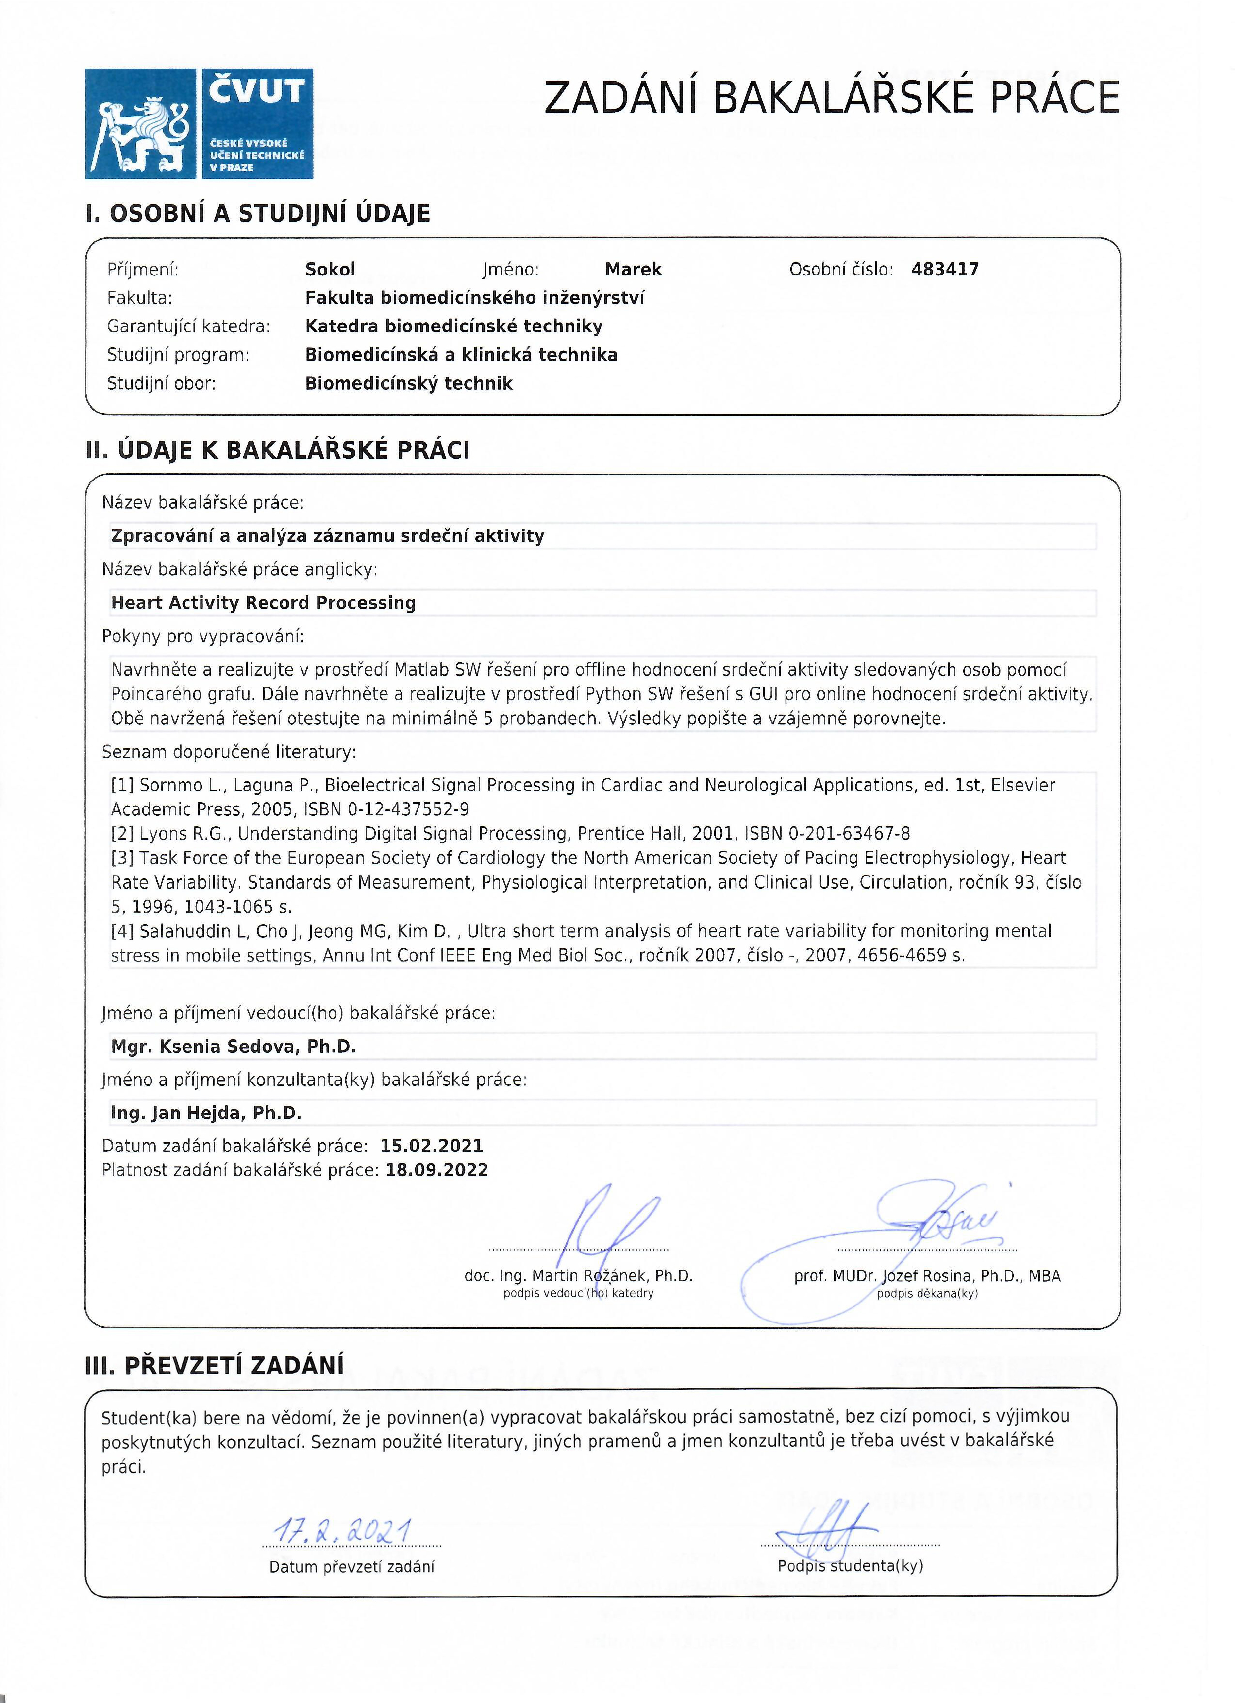
\includepdf[pages=-, trim=1mm 1mm 6mm 1mm, clip]{assignment/assignment_colored}

\null\vfill
\section*{Prohlášení}
% \hspace ruší odsazení odstavce - v šabloně u prohlášení odstavce odsazené nejsou. 
Prohlašuji, že jsem bakalářskou práci s názvem \uv{\nazev} vypracoval/a samostatně a~použil/a k~tomu úplný výčet citací použitých pramenů, které uvádím v seznamu přiloženém k~bakalářské práci.

\hspace{-0.75cm}Nemám závažný důvod proti užití tohoto školního díla ve smyslu \S 60 Zákona č.121/2000~Sb., o~právu autorském, o~právech souvisejících s právem autorským a~o~změně některých zákonů (autorský zákon), ve znění pozdějších předpisů.

\vspace{1em}

\hspace{-0.75cm}V Kladně dne \ldots \ldots \ldots \hfill \ldots \ldots \ldots \ldots \ldots \ldots \ldots \ldots \ldots \ldots

\hspace{10cm} \textbf{\autor}

\clearpage

\null\vfill
\section*{Poděkování}
% Mé poděkováni patři též XXXXXXXX za spolupráci při získávání údajů pro výzkumnou část práce.
Rád bych poděkoval vedoucí své bakalářské práce, Mgr. Ksenii Sedové, Ph.D. za
odborné vedení práce, za pomoc, vstřícnost a rady při zpracování této práce.
Dále bych rád poděkoval panu Ing et Ing. Janu Hejdovi, Ph.D. za všestrannou
pomoc, množství cenných a inspirativních rad, podnětů, doporučení a čas, který
mi věnoval při řešení dané problematiky. V neposlední řadě děkuji své rodině a
všem přátelům, kteří mě při vytváření této práce podpořili.

\clearpage


\null\vfill
\section*{ABSTRAKT}
\subsection*{\nazev:}
Bakalářská práce se věnuje návrhu a realizaci softwarového řešení pro hodnocení
srdeční aktivity v programovém prostředí MATLAB a Python. Hlavním cílem je
navrhnout adaptivní algoritmus, který bude schopný realizovat analýzu na
naměřeném EKG signálu zatíženého artefakty a dále aplikovat tuto metodu pro
měření v reálném čase. Pro hodnocení zpracovaného záznamu byla vybraná analýza v
časové oblasti, konkrétně variabilita srdeční frekvence a z ní vycházející
parametry. Dalším cílem práce je vizualizace výstupu v podobě interaktivních
grafů zobrazujících ve vybraných časových úsecích Poincarého graf. K testování
navrženého řešení byly použity krátkodobé záznamy naměřené celkem u 5 probandů.
Během měření byli probandi v prostředí virtuální reality, ve které byl každý z
nich vystaven situaci stimulující kognitivní zátěž a monitorován přenosným
elektrokardiografem neboli Holterovsky. Výsledkem práce je sada skriptů
implementovaných v prostředí Matlab schopných offline adaptivně zpracovat EKG a
zobrazit grafy parametrů prokazujících korelaci kognitivní zátěže s variabilitou
srdečního rytmu v závislosti na čase. Byla naprogramována multiplatformní Python
GUI aplikace rozšiřující výstup v rámci online měření.
\subsection*{Klíčová slova}
EKG (Elektrokardiogram), zpracování EKG, detekce EKG komponentů, EKG analýza, HRV analýza, HRV parametry, MATLAB, Python
\clearpage


\null\vfill
\section*{ABSTRACT}
\subsection*{\nazevENG:}
The bachelor's thesis deals with the design and implementation of a software
solution for the evaluation of cardiac activity in the MATLAB and Python
software environment. The main goal is to design an adaptive algorithm in the
MATLAB environment, that will be able to perform offline analysis on the
measured ECG signal loaded with artifacts using a Poincaré graph. For the
evaluation of the processed records, the analysis in the time domain was
selected, specifically the variability of the heart rate and the parameters
based on it. Another goal of this work is to design and implement a solution
with a GUI for online evaluation of cardiac activity in the Python environment.
For testing of the proposed solution, short-term records measured in a total of
5 probands were used. During the measurement, the probands were first at rest
and then each of them was exposed to a situation that stimulates cognitive
stress. Each of the probands was monitored during the measurement by Holter, a
portable electrocardiogram. The result of the work is a set of scripts
implemented in the MATLAB environment capable to adaptively process the ECG
offline and display graphs of the parameters demonstrating the correlation of
cognitive load with heart rate variability over time. A multiplatform Python GUI
application was programmed to extend the output for online measurement. 
\subsection*{Key words}
ECG (Electrocardiogram), ECG processing, detection of ECG components, ECG analysis, HRV analysis, HRV parameters, MATLAB, Python
\clearpage

\pagestyle{plain}	% Číslování stránek začíná odsud

\tableofcontents			% Vloží obsah

\clearpage

\section*{Seznam symbolů a zkratek} %sekce = nadpis, s * není v obsahu
\addcontentsline{toc}{section}{Seznam symbolů zkratek}
\subsection*{Seznam symbolů}

\begin{table}[H]
	\label{tab:symboly}
	\begin{center}
		\begin{tabular}{p{2.5cm}p{2.5cm}p{8.25cm}}
			\noalign{\hrule height 2pt}
			Symbol                      & Jednotka & Význam                                         \\
			\noalign{\hrule height 2pt}
			$A$                         & dB       & Zesílení                                       \\
			$a$                         & ms       & Šířka elispy                                   \\
			$\alpha$                    & -        & Škálovací faktor                               \\
			$b$                         & ms       & Výška elipsy                                   \\
			$Bc[n]$                     & mV       & Zpětně kumulovaný signál                       \\
			$\beta$                     & -        & Parametr Kaiserova okna                        \\
			$c_j$                       & -        & Koeficienty polynomiální regrese               \\
			$dRR$                       & -        & Normalizovaná časová série R-R intervalů       \\
			$dRRs$                      & s        & Časová série R-R intervalů                     \\
			$Fs$                        & Hz       & Vzorkovací frekvence                           \\
			$mRR$                       & -        & Normalizovaná časová série R-R intervalů       \\
			$mRRs$                      & s        & Časová série R-R intervalů                     \\
			$R$                         & s        & Časová hodnota vybrané R vlny                  \\
			$R_m$                       & ms       & Časová hodnota doplněné R vlny                 \\
			$R_{max}$                   & mV       & Amplituda vybrané R vlny                       \\
			$RR$                        & ms       & Časová série R-R intervalů                     \\
			$\overline{RR}$             & ms       & Průměrná hodnota R-R intervalů                 \\
			$\overrightarrow{RR_{i+1}}$ & s        & Časový vektor R-R intervalů pro osu Y          \\
			$\overrightarrow{RR_i}$     & s        & Časový vektor R-R intervalů pro osu X          \\
			$S11$                       & -        & Hodnoty subprostoru S1 pro osu X               \\
			$S12$                       & -        & Hodnoty subprostoru S1 pro osu Y               \\
			$S21$                       & -        & Hodnoty subprostoru S2 pro osu X               \\
			$S22$                       & -        & Hodnoty subprostoru S2 pro osu Y               \\
			$SD1$                       & ms       & Směrodatná odchylka hodnot hlavní osy elipsy   \\
			$SD2$                       & ms       & Směrodatná odchylka hodnot vedlejší osy elipsy \\
			$Th_{amp}$                  & mV       & Prahová amplituda                              \\
			$Th_{RR}$                   & ms       & Prahová délka R-R intervalu                    \\
			$Th1$                       & s        & Normalizační práh pro sérii $dRRs$             \\
			$Th2$                       & s        & Normalizační práh pro sérii $mRRs$             \\
			$w[n]$                      & -        & Koeficienty Kaiserova okna                     \\
			$W_i^{L,R}$                 & ms       & Plovoucí okno                                  \\
			$X$                         & ms       & Souřadnice elipsy pro osu X po rotaci          \\
			$x$                         & ms       & Souřadnice elipsy pro osu X                    \\
			$x[n]$                      & mV       & Originální signál                              \\
			$x1$                        & ms       & Hlavní osa elipsy                              \\
			$x2$                        & ms       & Vedlejší osa elipsy                            \\
			$Y$                         & ms       & Souřadnice elipsy pro osu Y po rotaci          \\
			$y$                         & ms       & Souřadnice elipsy pro osu Y                    \\
			$y[n]$                      & mV       & Hodnoty diferencovaného signálu                \\
			$y_j$                       & mV       & Hodnoty signálu po SGF filtraci                \\
			\noalign{\hrule height 2pt}
		\end{tabular}
	\end{center}
\end{table}

\clearpage

\subsection*{Seznam zkratek}
\begin{table}[h]
	\label{tab:zkratky}
	\begin{center}
		\begin{tabular}{p{2.5cm}p{11.25cm}}
			\noalign{\hrule height 2pt}
			Zkratka & Význam                                                                                                               \\
			\noalign{\hrule height 2pt}
			AI      & Umělá inteligence (Artificial intelligence)                                                                          \\
			ANS     & Autonomní nervová soustava (Autonomic nervous system)                                                                \\
			AP      & Akční potenciál (Action potential)                                                                                   \\
			AV      & Atrioventrikulární uzel                                                                                              \\
			CSV     & Čárkou oddělené hodnoty (Comma separated values)                                                                     \\
			DP      & Dolní propust                                                                                                        \\
			EKG     & Elektrokardiogram                                                                                                    \\
			EMG     & Elektromyogram                                                                                                       \\
			FFT     & Rychlá Fourierova transformace (Fast Fourier transform)                                                              \\
			FIR     & Filtr s konečnou impulzní odezvou (Finite impulse response)                                                          \\
			GUI     & Grafické uživatelské rozhraní (Graphical User Interface)                                                             \\
			HF      & Vysoké frekvence (High frequency)                                                                                    \\
			HP      & Horní propust                                                                                                        \\
			HR      & Srdeční frekvence (Heart rate)                                                                                       \\
			HRV     & Variabilita srdeční frekvence (Heart rate variability)                                                               \\
			IIR     & Filtr s nekonečnou impulzní odezvou (Infinite impulse response)                                                      \\
			LF      & Nízké frekvence (Low frequency)                                                                                      \\
			LTI     & Lineární časově invariantní systém (Linear time-invariant system)                                                    \\
			NVI     & Neuroviscerální integrace (Neurovisceral integration)                                                                \\
			PNS     & Parasympatický nervový systém                                                                                        \\
			PP      & Pásmová propust                                                                                                      \\
			PSS     & Převodní systém srdeční                                                                                              \\
			RMSSD   & Odmocnina průměru umocněných rozdílů po sobě jdoucích N-N intervalů (Root mean square of the successive differences) \\
			SA      & Sinoatriální uzel                                                                                                    \\
			SD      & Směrodatná odchylka (Standard deviation)                                                                             \\
			SDNN    & Standardní odchylka všech N-N intervalů (Standard deviation of the N-N intervals)                                    \\
			SNS     & Sympatický nervový systém                                                                                            \\
			SW      & Software                                                                                                             \\
			SVT     & Supraventrikulární tachykardie (Supraventricular tachycardia)                                                        \\
			VLF     & Velmi nízké frekvence (Very frequency)                                                                               \\
			VNS     & Vegetativní nervová soustava (Vegetative nervous system)                                                             \\
			WLAN    & Bezdrátová lokální síť (Wireless local area network)                                                                 \\
			\noalign{\hrule height 2pt}
		\end{tabular}
	\end{center}
\end{table}
\clearpage

%\addcontentsline{toc}{section}{Seznam tabulek}
%\listoftables 		% seznam tabulek

%\clearpage 			% konec stránky a odskok na další

%\addcontentsline{toc}{section}{Seznam obrázků}
%\listoffigures 		% seznam obrázků
%\clearpage

%\addcontentsline{toc}{section}{Seznam algoritmů}
%\listofalgorithms
%\clearpage


\section{Úvod}
Záznam srdeční aktivity neboli elektrokardiogram (EKG), na kterém je vidět
časový průběh změn elektrického potenciálu srdce, hraje velmi důležitou roli v
kardiologické diagnostice. Uchovává v sobě komponenty jak v časové, tak i ve
frekvenční doméně, díky kterým lze realizovat EKG analýzu, a to i za jinými
účely než jen z hlediska kardiologie. Aby bylo možné analýzu provést či
extrahovat potřebné komponenty, musí se signál patřičně zpracovat, jelikož jeho
surová podoba může být zkreslená a často obsahuje mnohočetné nežádoucí
artefakty.

Důležitými východisky, od kterých se odvíjí následně zvolená metodika při
zpracování signálu a tím pádem i samotný výstup, jsou zejména kvalita a
charakteristika biosignálu. V ideálním případě se nabízí myšlenka univerzálního
způsobu, který signál spolehlivě zbaví všech nežádoucích elementů nehledě na
zmíněné východiska. Jelikož v posledních letech nastal velký průlom v oblasti
využití strojového učení (machine learning) a umělé inteligence (AI, artificial
inteligence) pro zpracování biosignálů, tak úvaha v rámci metod z těchto oblastí
může právě k takové zavádějící myšlence vést. V praxi se ale při zpracování EKG
signálu neorientuje jen jeho kvalitou či charakterem ale také povahou
nadcházející analýzy. Proto se při zpracování využívají variace, kombinace a
obdoby konvenčních metod, kde je každá volena na základě zvolené dílčí oblasti
analýzy nebo jiných specifických požadavků. Průnik všech metod obsahuje v první
řadě snahu o efektivní potlačení nežádoucích prvků a odkrývá tak část
problematiky této práce.

Při samotném základním EKG vyšetření srdce, zde hraje roli několik vnějších i
vnitřních vlivů, které se ve výsledku mohou jevit jako stěžejní při zpracovávání
biosignálu. Takové jevy se nazývají nežádoucími prvky. Těmi jsou zejména
elektrické a magnetické vlastnosti tkání, zvláště svalový akční potenciál (AP),
nebo umístění a vodivost elektrod využívaných při vyšetření. Proto je velmi
důležité signál pečlivě analyzovat a filtrovat exaktními metodami, jinak by jeho
použití mohlo vést k vágním výsledkům. 

Po správném zpracování EKG signálu je možné začít s jeho analýzou. Její
interpretace umožňuje detekovat potencionální srdeční vady či jiné srdeční
stavy. Dále se může pracovat s extrahovanými komponenty, s jejichž pomocí lze
například určit variabilitu srdečního rytmu (HRV, Heart rate variability). Tato
specifická metrika a analýza jejích parametrů má pro nás mnoho dalších
klinických významů a umožňuje využití nejen v rámci kardiologie ale také
neurologie a psychofyziologie.

Tato práce se zaměřuje na problematiku týkající se zpracování a analýzy EKG
signálu, a to nejen v rámci naměřených signálů (offline) ale také při měření v
reálném čase (online). Vybranou dílčí oblastí analýzy je především hodnocení
kognitivní zátěže pomocí HRV a Poincarého grafu s jeho parametry, vypočtenými v
časové oblasti, které jsou založené na intervalech mezi jednotlivými údery
srdce.

\clearpage

\section{Přehled současného stavu}
Přehled současného stavu se věnuje základnímu anatomickému popisu srdce společně
s úvodem do jeho fyziologie a elektrofyziologie ve spojení s neurofyziologickými
vlivy. Dále jsou zde popsány principy vyšetřovacích metod v kardiologii,
konkrétně oblast měření, zpracování a hodnocení elektrického záznamu srdeční
aktivity. Závěr kapitoly je věnován detailnějšímu rozboru variability srdeční
frekvence, která je předmětem analýzy zpracovaného EKG záznamu v rámci této
práce.

\subsection{Srdce}
\label{section:heart}
Srdce (cor) je orgán nepravidelného kuželovitého tvaru velkého zhruba jako pěst
dospělého člověka, skládající se převážně ze svaloviny~\cite{Memorix2017}. Tato
pravidelně oscilující pumpa zastupuje v kardiovaskulárním systému funkci
krevního čerpadla, které umožňuje setrvalou perfuzi orgánů a tkání organismu.
Nachází se ve střední částí hrudní dutiny (cavitas thoracica) mezi pravou a
levou pleurální blánou (pleura mediastinalis dextra et sinistra) v prostoru za
sternem nazývaném mediastinum.~\cite{Weinhaus2005}.

\begin{figure}[h]
	\begin{center}
		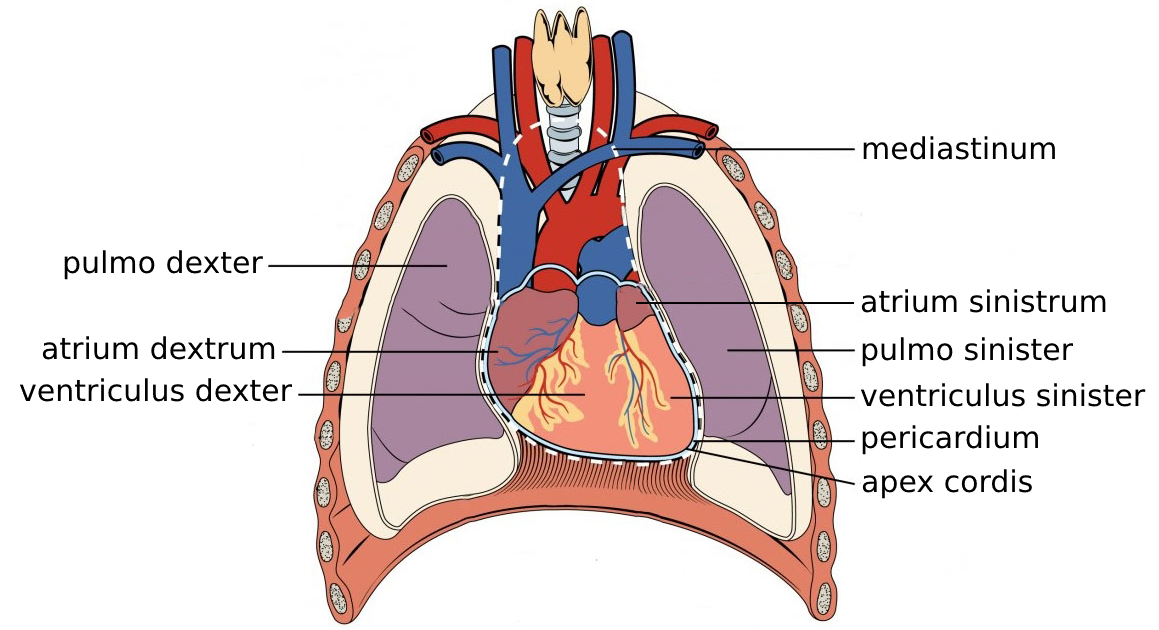
\includegraphics[width=0.7\textwidth]{anatomy/mediastinum}
		\caption{Umístění srdce v hrudní dutině mezi plícemi v mediastinu
			(Upraveno a převzato z~\cite{OpenStax})}
		\label{fig:mediastinum}
	\end{center}
\end{figure}

\subsubsection{Struktura srdce}
\label{section:heart_structure}
Struktura srdce je tvořena dvěma síněmi (atrium dextrum et sinistrum) a dvěma
komorami (ventriculus dexter et sinister), oddělenými mezikomorovou přepážkou
(septum interventriculare), která současně rozděluje srdce na levé a
pravé~\cite{Memorix2017}. O tok krve srdcem se starají čtyři srdeční chlopně,
fungující jako jednosměrné ventily (Obr.~\ref{fig:heartanatomy}). Z komory
pravého srdce je přečerpávána neokysličená krev do plic. Z komory levého srdce
se pumpuje okysličená krev do celého krevního oběhu, a proto je svalovina levé
komory silnější. Rozdíl zde není jen ve svalovině ale také v krevním tlaku.
Pumpování krve do tělního oběhu vyžaduje mnohem větší tlak než do plicního
oběhu. Rozlišuje se malý a velký oběh neboli krevní cirkulace pulmonální a
systémová. Systematicky k této cirkulaci dochází díky řetězci opakujících se
elektrických a mechanických událostí, uskutečněných během jedné časové periody,
nazývané srdeční cyklus (srdeční revoluce). Konkrétně se jedná o svalovou
kontrakci (systola) a svalovou relaxaci (diastola). Blíže je tento cyklus popsán
v sekci~\ref{section:cardiac_cycle}. Průtok krve srdcem je znázorněn pomocí
bílých šipek na Obr.~\ref{fig:heartanatomy}~\cite{Stejfa2006}.

\begin{figure}[h]
	\begin{center}
		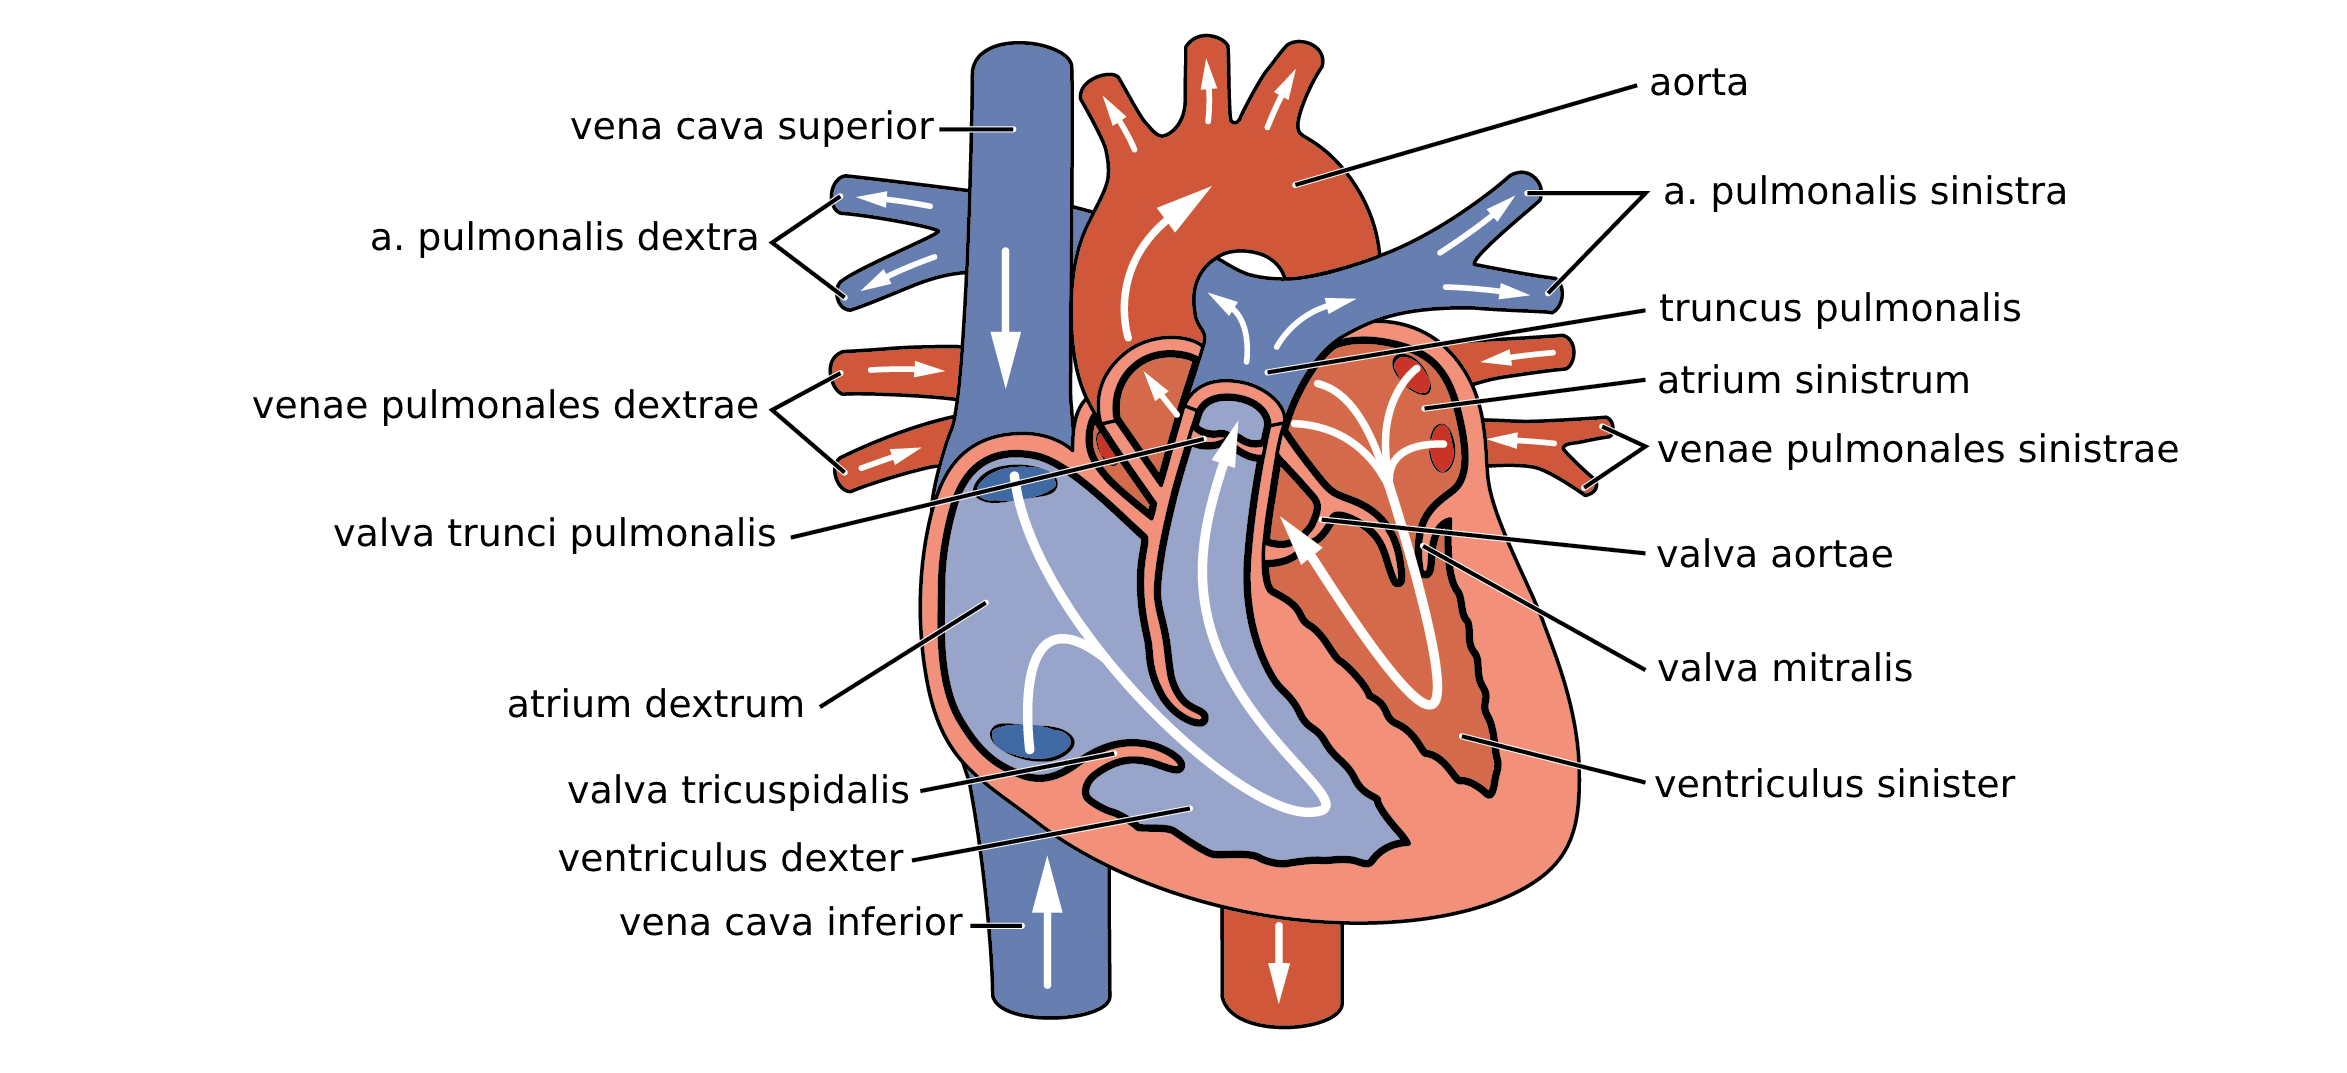
\includegraphics[width=1\textwidth]{anatomy/heart}
		\caption{Schéma srdce (anteriorní řez) zobrazující tok krve srdcem
			prostřednictvím bílých šipek (Upraveno a převzato
			z~\cite{OpenStax})}
		\label{fig:heartanatomy}
	\end{center}
\end{figure}

Vnější část srdce, obdobně jako u cév, sestává ze tří vrstev: myokard (tunica
media), endokard (tunica intima) a epikard (tunica serosa), které společně tvoří
mohutný segment srdeční stěny~\cite{Memorix2017}. Myokard (myocardium), nejširší
část srdeční stěny podléhající kontrakcím, je tvořen v závislosti na srdečním
oddílu dvěma až třemi vrstvami příčně pruhované svaloviny. Na myokard naléhá
silná řídká vrstva kolagenního vaziva a tuku neboli epikard (epicardium), ve
kterém probíhají cévy zásobující srdce. Poslední vrstvou, která vystýlá srdeční
dutiny, a mezi síněmi a komorami tvoří mitrální chlopně, je endokrad
(endocardium). Povrch srdce obaluje vazivově-serózní blána, osrdečník
(pericardium). Prostor mezi perikardem a epikardem je vyplněn malým množstvím
serózní tekutiny, která umožňuje jejich vzájemný klouzavý pohyb. Tento prostor
se nazývá perikardiální dutina (cavitas
pericardialis)~\cite{Weinhaus2005,Dylevsky2013}.

\begin{figure}[h]
	\begin{center}
		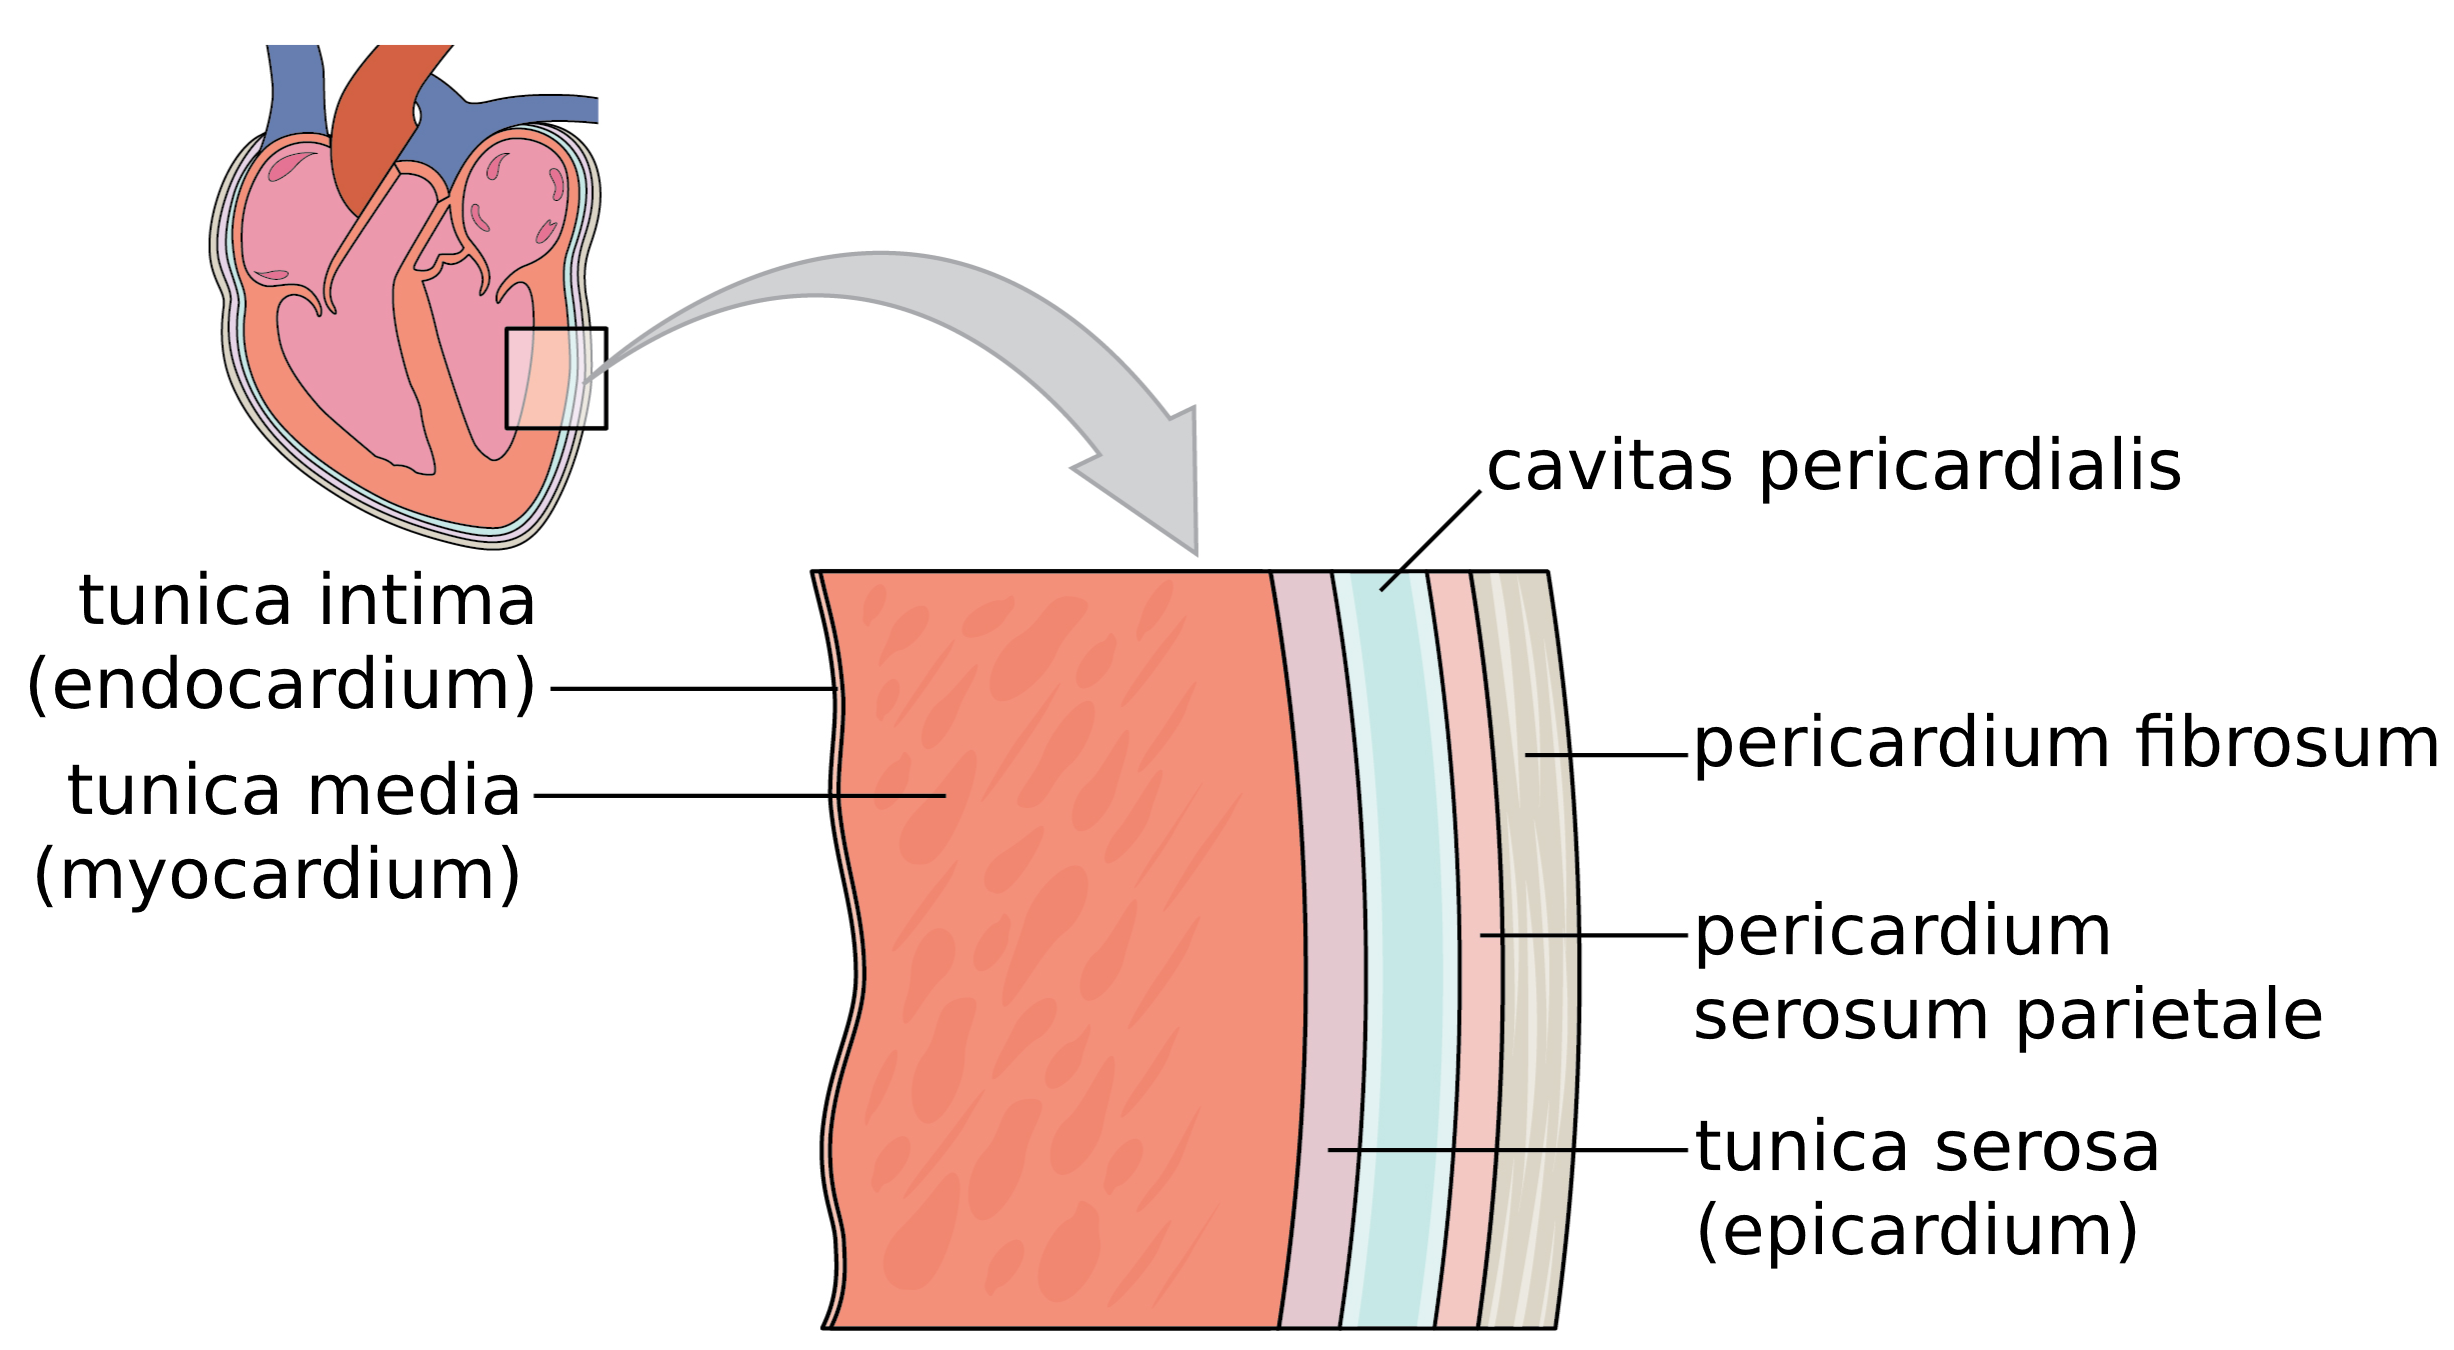
\includegraphics[width=0.7\textwidth]{anatomy/heart_muscle}
		\caption{Perikardiální membrána a vrstvy srdeční stěny (Upraveno a
			převzato z~\cite{OpenStax})}
		\label{fig:heartlayers}
	\end{center}
\end{figure}

Obecně se srdeční svalovina skládá z příčně pruhované srdeční tkáně. K zajištění
srdeční činnosti obsahuje ale myokard kromě svalových buněk schopných kontrakce
(pracovní myokard) také specializované kardiomyocyty, které se podílejí na
tvorbě převodního systému srdečního (PSS)~\cite{Memorix2017,Dylevsky2013}. Tento
systém, společně ve spojení s autonomním nervovým systémem~(ANS), tvoří pro tuto
práci zásadní část, a proto je podrobněji probrán v samostatné kapitole.

\subsubsection{Srdeční cyklus}
\label{section:cardiac_cycle}
Jak již bylo naznačeno v kapitole~\ref{section:heart_structure}, dvě z hlavních
funkcí srdce jsou: přečerpat neokysličenou krev ze systémového oběhu do plic,
kde dojde k její oxygenaci, a pumpovat okysličenou krev z plic zpět do všech
tkání, kde dojde znovu k její deoxygenaci. Celý proces se kontinuálně znovu
opakuje. Srdeční cyklus je tedy časově sladěný průběh dvou hlavních fází
začínající systolou a končící diastolou~\cite{Weinhaus2005}. Systola je okamžik,
kdy je ze srdce kontrakcí a za vysokého tlaku vypuzována krev do oběhu, zatímco
při diastole neboli plnící nízkotlaké fází, se srdce plní krví. Síně i komory
podléhají oběma těmto fázím a jsou koordinované otevíráním a zavíráním
atrioventrikulárních a semilunárních chlopní. Zároveň je regulována i čerpací
funkce srdce tak, aby v každém momentu byly splněny nároky tkání na okysličenou
krev~\cite{OpenStax}. Na Obr.~\ref{fig:cardiac_cycle_ecg} lze vidět průběh EKG
křivky ve vztahu se srdečním cyklem (srdeční revolucí).

\begin{figure}[h]
	\begin{center}
		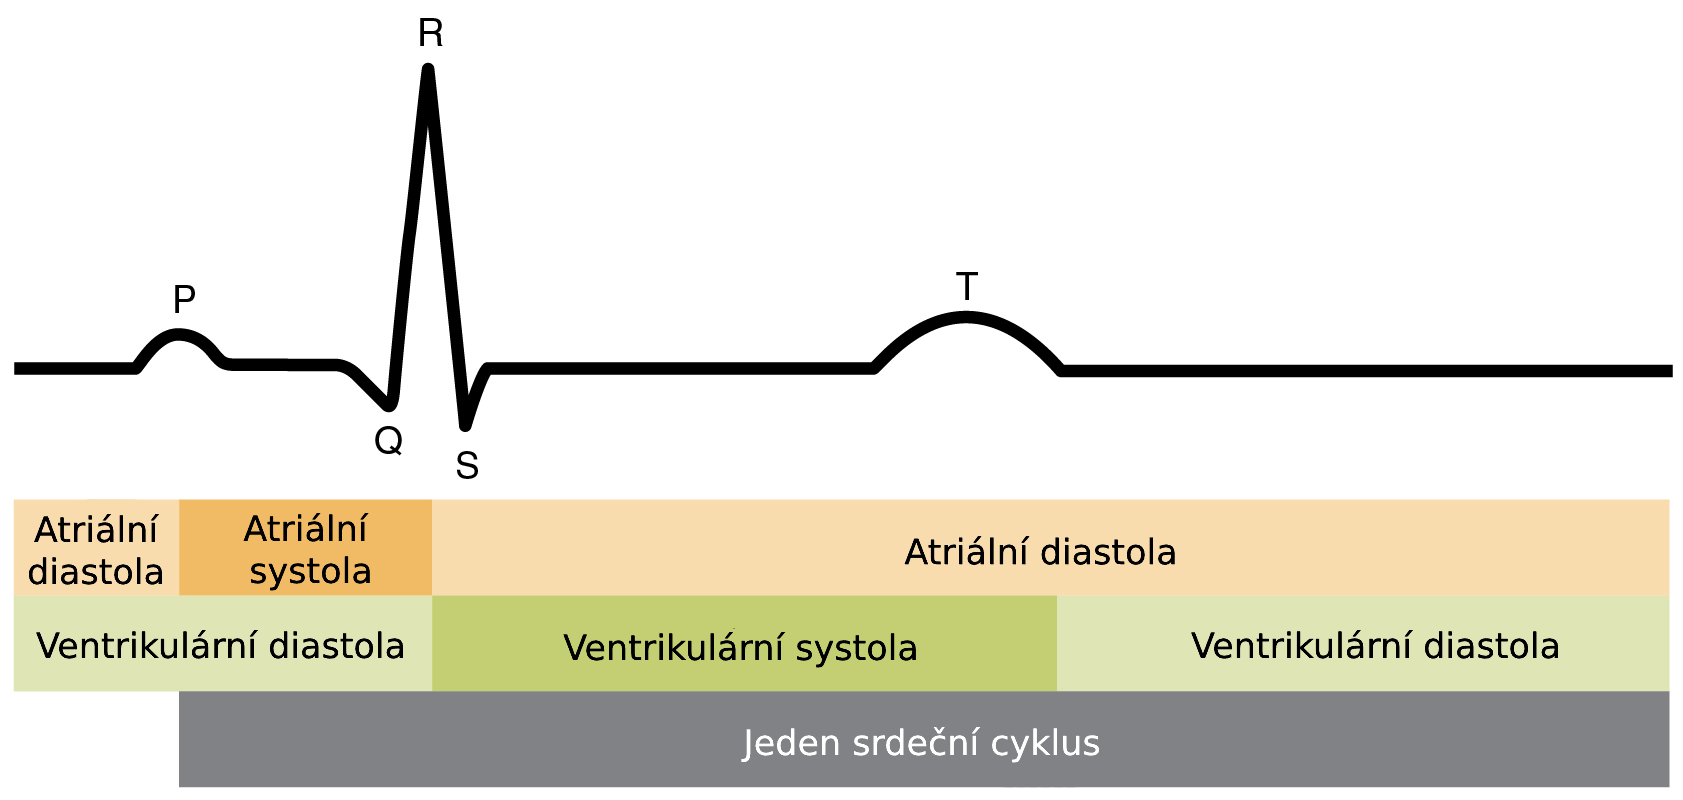
\includegraphics[width=0.85\textwidth]{anatomy/cardiac_cycle_ecg}
		\caption{Vztah srdečního cyklu s EKG (Upraveno a převzato
		z~\cite{OpenStax})}
		\label{fig:cardiac_cycle_ecg}
	\end{center}
\end{figure}

\subsubsection{Převodní systém srdeční}
\label{section:pss}
Anatomicky se převodní systém srdeční skládá ze sinoatriálního uzlu (SA uzel,
nodus sinoatrialis), atrioventrikulárního uzlu (AV uzel, nodus
atrioventricularis), síňokomorového svazku (Hisův svazek, fasciculus
atrioventricularis) s jeho raménky (Tawarova raménka, crus dextrum et sinistrum
fasciculi atrioventricularis) a koncovými vlákny (Purkyňova vlákna, rami
subendocardiales), které končí ve svalovině komor. Stavba PSS je vyznačena na
Obr.~\ref{fig:pss}~\cite{Dylevsky2013}.

\begin{figure}[h]
	\begin{center}
		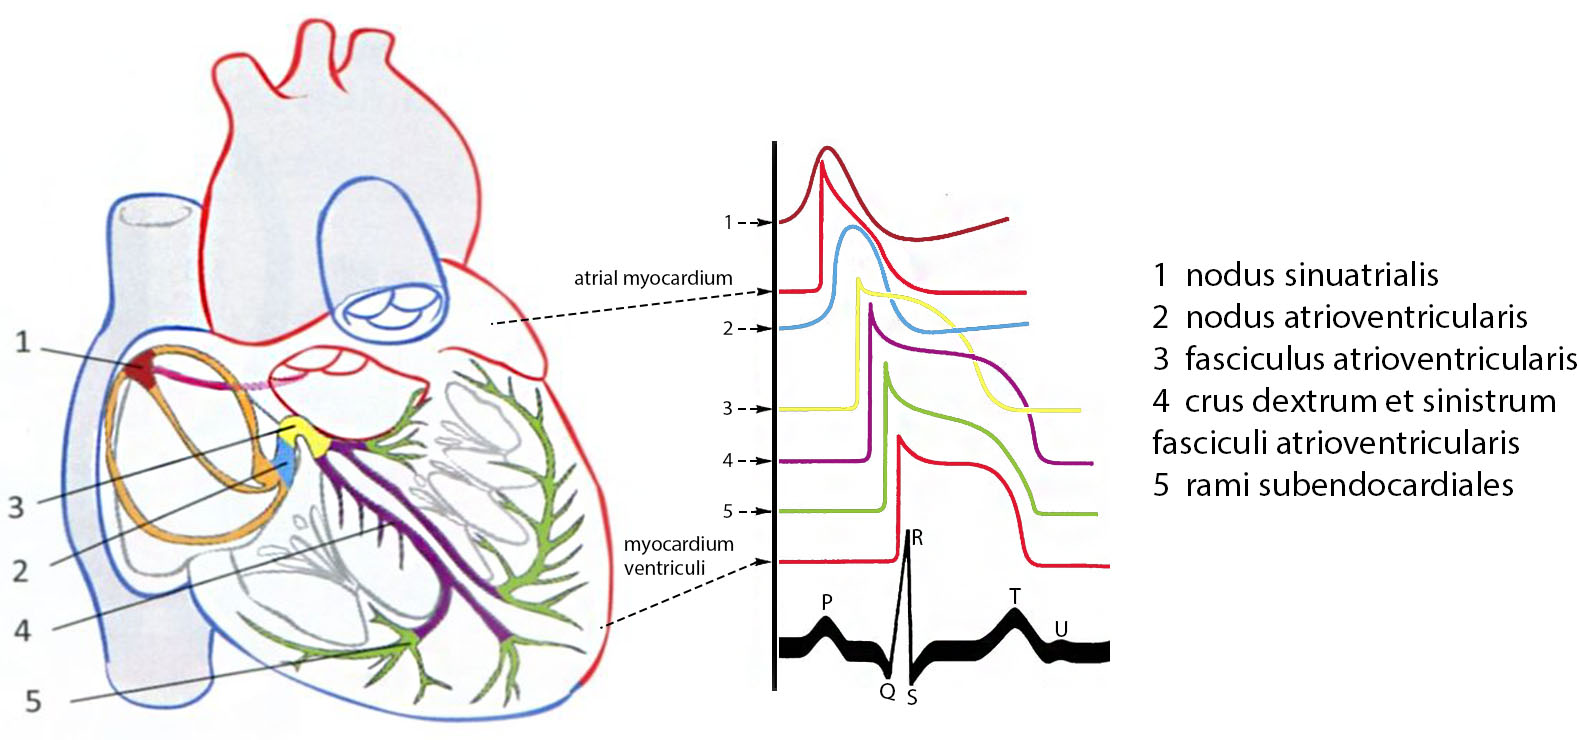
\includegraphics[width=0.9\textwidth]{anatomy/pss}
		\caption{Převodní systém srdeční (Upraveno a převzato
		z~\cite{ecgpediaConduction})}
		\label{fig:pss}
	\end{center}
\end{figure}

Z funkčního hlediska se jedná o soubor specializovaných částí myokardu. První
část tvoří buňky pracovního myokardu, jejichž hlavním úkolem je
kontrakce~\cite{Cihak2016}. Druhou část reprezentují specializované buňky
převodního srdečního systému -- kardiomyocyty -- které jsou morfologicky těžko
odlišitelné od buněk pracovního myokardu. Funkčně ale mají navíc na starosti
autonomní generaci akčního potenciálu (AP), rychlé vedení vzruchu elektrického
charakteru za účelem podráždění myokardu (excitabilita) a vyvolání jeho stahu
(systola). Ke vzniku těchto vzruchů dochází uvnitř orgánu (automacie) a poté se
šíří dále napříč srdeční svalovinou. 

Buňky srdeční svaloviny jsou navzájem propojeny interkalárními disky (disci
intercalares). Součástí disků jsou tzv. \textit{gap junctions} neboli
specializované struktury zajišťující převod impulsu mezi kardiomyocyty. V
místech, kde toto propojení nevzniká jsou spoje mezi jednotlivými buňkami
zajištěny desmozomy a nexy, které umožňují jejich vzájemnou
komunikaci~\cite{Dylevsky2013, Stejfa2006}.

Srdce, konkrétně srdeční svalovinu (myokard) spolu s PSS tedy charakterizuje
několik hlavních funkcí \cite{Stejfa2006}:
\begin{itemize}
	\item \textit{Automacie (chronotropie, samočinnost)} -- samočinná rytmická
	      generace elektrických impulzů pacemakerovými buňkami k podnícení
	      pravidelné kontrakce,
	\item \textit{Excitabilita (bathmotropie, dráždivost)} -- reakce na
	      podráždění elektrickým impulzem depolarizací,
	\item \textit{Konduktivita (dromotropie, vodivost)} -- vedení vzniklých
	      elektrických vzruchů celou srdeční svalovinou,
	\item \textit{Stážlivost (inotropie, kontraktilita)} -- mechanická odpověď
	      kontraktilních buněk pracovního myokardu na vzniklé elektrické
	      podněty.
\end{itemize}

Ve zmíněných dvou funkčních částech je také potřeba rozlišovat rozdíly na
buněčné úrovni, a to konkrétně v rámci membránových potenciálů. 

Buňky pracovního myokardu za normálních podmínek ve zdravém srdci nevyužívají
schopnost samovolně vytvářet vzruchy. Dráždění buněk vyvolává šíření akčního
potenciálu srdeční svalovinou, což má za následek zahájení kontrakce myokardu.
Klidový membránový potenciál buněk se pohybuje okolo -90~\si\mV. Změnou klidového
membránového potenciálu vzniká akční potenciál, jehož časový průběh sestává z
následujících fázi: rychlá depolarizace (fáze 0), časná repolarizace (fáze 1),
plató akčního potenciálu (fáze 2), konečná repolarizace (fáze 3) a návrat ke
klidovému potenciálu (fáze 4)~\cite{Petrek2019}.
\begin{figure}[h]
	\centering
	\begin{subfigure}{0.4\textwidth}
		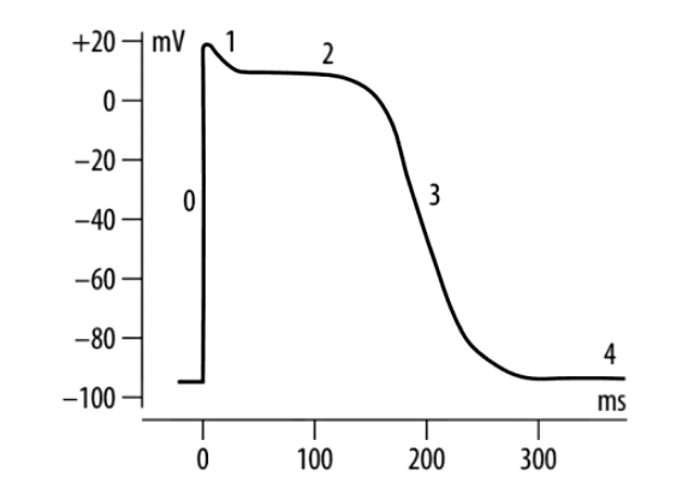
\includegraphics[width=1\textwidth]{anatomy/myokard_ap}
		\caption{Akční potenciál buňky pracovního myokardu~\cite{Petrek2019}}
		\label{fig:myokard_ap}
	\end{subfigure}
	\hfil
	\begin{subfigure}{0.5\textwidth}
		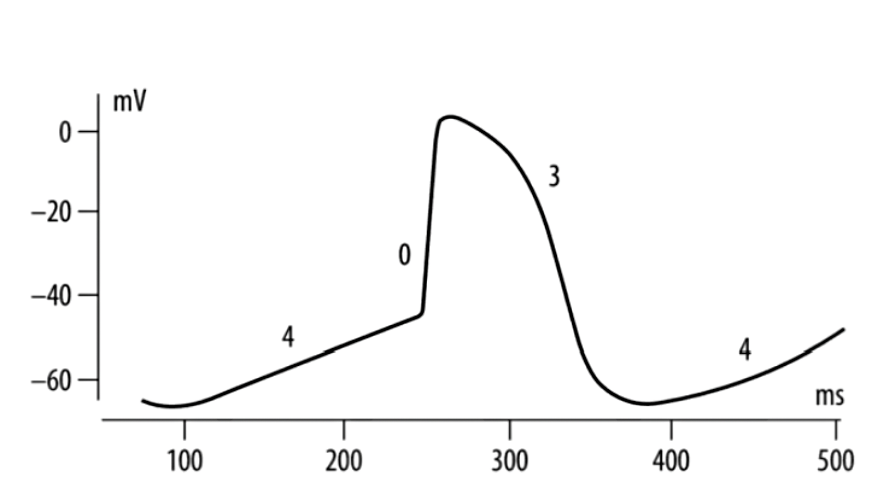
\includegraphics[width=1\textwidth]{anatomy/pss_ap}
		\caption{Akční potenciál buňky převodního systému
		srdce~\cite{Petrek2019}}
		\label{fig:pss_ap}
	\end{subfigure}
	\caption{Rozdíl průběhů akčních potenciálu pracovního myokardu a převodního
		systému srdce: 0 -- rychlá depolarizace, 1 -- časná repolarizace, 2 --
		plató akčního potenciálu, 3 -- konečná repolarizace, 4 -- návrat ke
		klidovému potenciálu}
	\label{fig:ap}
\end{figure}
Klidový membránový potenciál pacemakerových buněk -- buněk SA a AV uzlu -- je
více depolarizován, než u buněk pracovního myokardu (-50 až -70 mV) a samovolně
klesá k prahové hodnotě (spontánní diastolická depolarizace). Jakmile klidový
potenciál dosáhne prahové hodnoty, vzniká další akční potenciál. Průběh akčního
potenciálu se od buněk pracovního myokardu také liší. Chybí zde 1. a 2. fáze.
Grafy akčních potenciálů jsou na Obr.~\ref{fig:ap}~\cite{Petrek2019}.

Elektrické vzruchy, vyvolávající rytmické smršťování srdečního svalu, primárně
vznikají v SA uzlu, uloženém při ústí horní duté žíly ve stěně pravé síně. Tento
uzel je udavatel srdečního rytmu (HR) neboli primární pacemaker. Iniciuje
atriální depolarizaci (kontrakce síní) -- vznik P vlny -- a vzruchy se z něj
šíří dále systémem. Než jsou tyto impulzy převedeny přes Hisův svazek na
Purkyňova vlákna, prochází vzruch AV uzlem (sekundární pacemaker), kde dochází k
jeho zpomalení a tvorbě časové prodlevy. Následkem jsou postupné kontrakce síní
a komor. Kontrakci komor (ventrikulární depolarizace) charakterizuje vznik QRS
komplexu na EKG křivce, který za fyziologických podmínek a normálního sinusového
rytmu sestává ze tří vln (viz Obr.~\ref{fig:cardiac_cycle_ecg}~a~\ref{fig:pss}):
\begin{itemize}[noitemsep]
	\item \textbf{Q vlna} -- počáteční negativní kmit komplexu
	\item \textbf{R vlna} -- pozitivní kmit komplexu
	\item \textbf{S vlna} -- negativní kmit komplexu následující po R vlně
\end{itemize}

Po ventrikulární depolarizaci nastává komorová repolarizace a vzniká T vlna.
Spojení mezi SA uzlem a AV uzlem je realizováno internodálními síňovými spoji,
vlákny stejného charakteru jako u PSS. Tyto spoje umožňují rozvádět vzruchy z SA
uzlu rychleji než samotná svalovina síní. Vzruchy je pak možno mezi síněmi a
komorami vést pomaleji či rychleji, což představuje jeden z regulačních
mechanismů srdeční frekvence~\cite{Dylevsky2013,Cihak2016}.

Tento sled, pravidelnost srdečního rytmu a proměnlivost srdečních akcí vůči
změnám v organismu, zajišťuje několikastupňový regulační systém. Zachycením
elektrických potenciálů v čase vzniká tzv. elektrokardiogram (EKG), na
kterém lze vidět průběh elektrického srdečního cyklu s jeho jednotlivými fázemi
(Obr.~\ref{fig:pss} -- P, Q, R, S, T)~\cite{Dylevsky2013,Cihak2016}.


\subsubsection{Regulace srdeční frekvence}
\label{section:hr_regulation}
Změny v srdeční frekvenci (chronotropie) a její variabilitě jsou jedním z
následků regulace srdeční činnosti, která mimo jiné ovliňuje také inotropii,
dromotropii a bathmotropii. Regulaci se v závislosti na místě průběhu
regulačního děje dělí na dvě úrovně, a to na intrakardiální a extrakardiální.
Intrakardiální regulační děje probíhají v srdci samotném, například následkem
mechanických změn myokardu. Blíže tyto děje popisuje Starlingův zákon nebo
Bainbridgeův reflex~\cite{Kittnar2020}. Extrakardiální děje se dále dělí na
nervové a humorální. Jelikož je srdeční frekvence řízena hlavně nervově, tak se
tato kapitola věnuje podrobněji extrakardiálním vlivům~\cite{Orel2019}.

\paragraph*{\textit{Nervová regulace srdečního rytmu}\\} Srdce je inervované
autonomním (vegetativním) nervovým systémem, konkrétně pregangliovými
parasympatickými vlákny (rami cardiaci nervi vagi) z bloudivého nervu (nervus
vagus) a sympatickými vlákny z krčního kmene sympatiku (n. cardiacus cervicalis
superior, medius et inferior), společně s větvemi jeho horního hrudního úseku
(nn. cardiaci thoracici)~\cite{Dylevsky2013,Kittnar2020}. Tato vlákna realizují
regulační děje, vzniklé na úrovní prodloužené míchy (medulla oblongata) v
kardioexcitačním nebo kardioinhibičním centru. Inervace tohoto typu představují
jeden z vyšších stupňů regulačních mechanismů a jejich dráždění má vliv na
srdeční frekvenci a její variabilitu~\cite{Dylevsky2013,Trojan2002}.

\begin{figure}[h]
	\begin{center}
		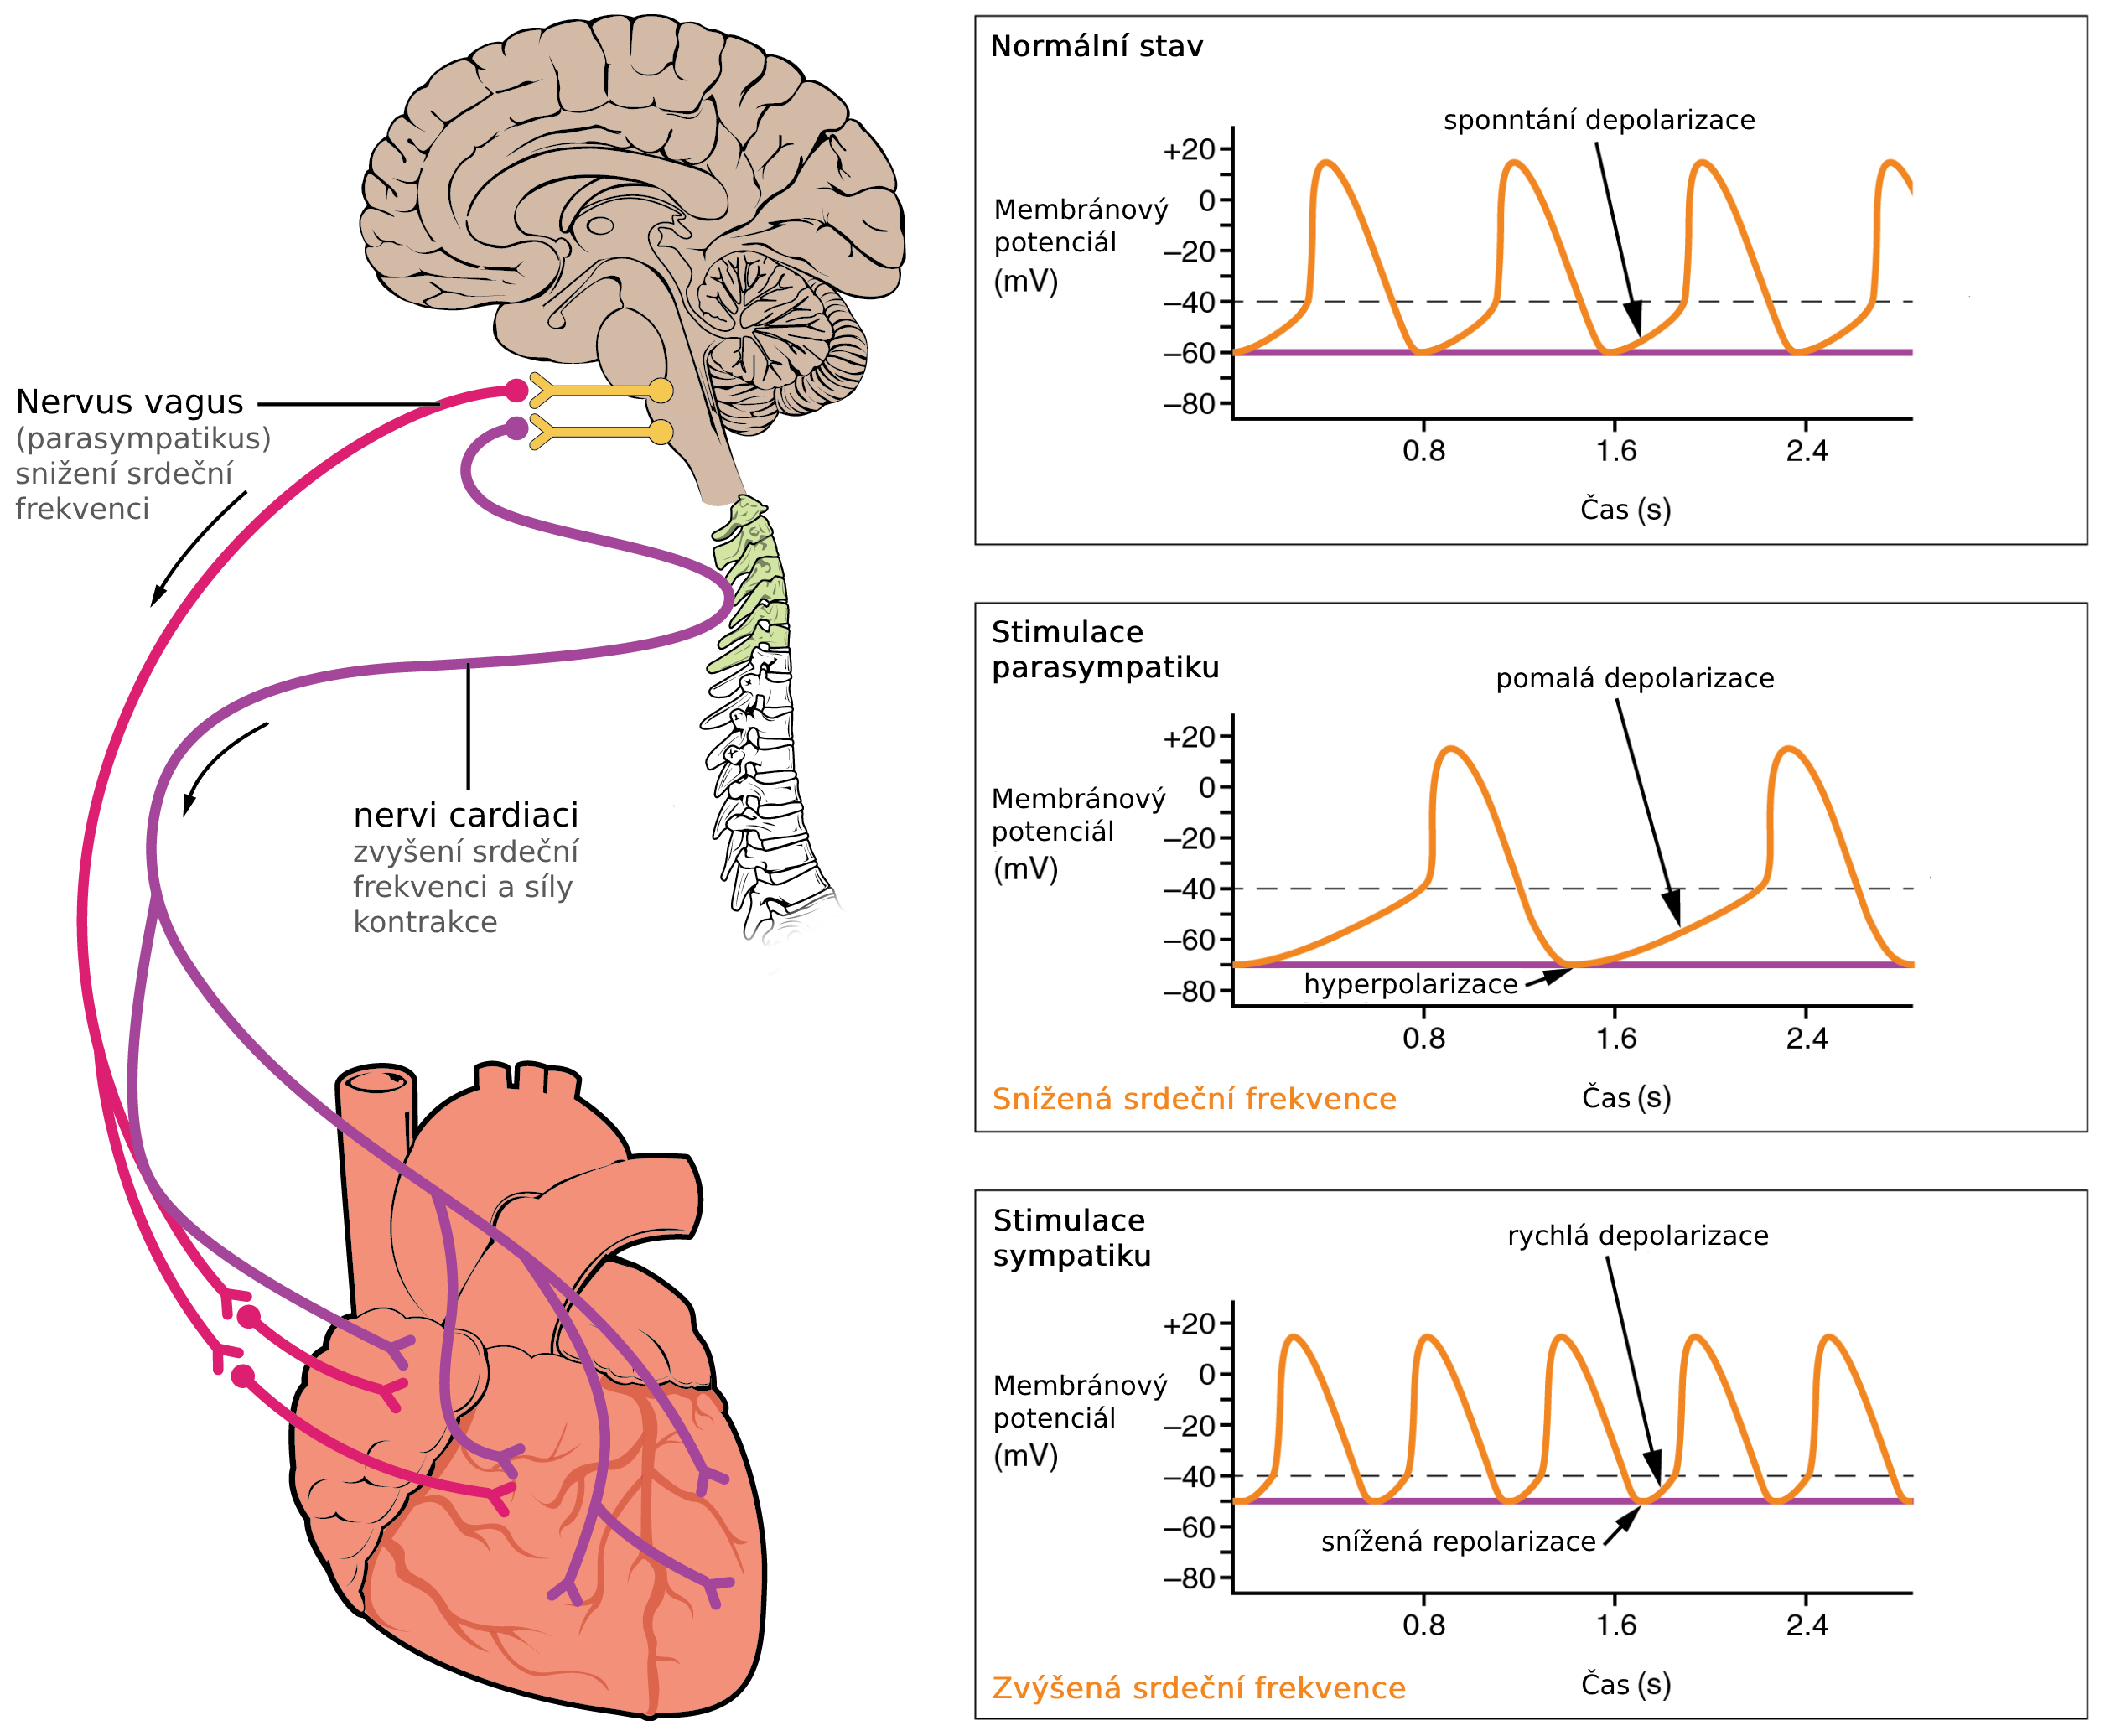
\includegraphics[width=1\textwidth]{anatomy/hr_regulation}
		\caption{Autonomní inervace kardioexcitačních a kardioinhibičních
			oblastí nacházejících se v prodloužené míše a jejich vliv na
			normální sinusový rytmus (Upraveno a převzato z~\cite{OpenStax})}
		\label{fig:hr_regulation}
	\end{center}
\end{figure}

Srdeční odezva na nervové podněty je realizována na nejnižší intrakardiální
úrovni pomocí srdečních ganglií, které se skládají z neuronů. Přesněji jsou to
hlavně cholingerní (vagální) a adrenergní (sympatické) srdeční neurony, sloužící
jako vagální spínací body se schopností reakce na chemické, mechanické a
elektrofyziologické podněty. Díky tomu může například nervová aktivita v
prefrontální kůře modulovat HRV (\ref{section:hrv}). Detailně tyto vztahy
popisuje model Neuroviscerální integrace (NVI)~\cite{Smith2017}.

Vliv parasympatiku je realizován uvolňováním mediátoru -- acetylcholinu -- z
koncových postgangliových vláken. Odpověď probíhá v srdeční tkání díky
muskarinovým cholingerním receptorům. Stimulací těchto receptorů se zpomaluje
proces spontánní diastolické depolarizace. Následkem je nižší srdeční rytmus
(negativní chronotropie) v SA uzlu a zpomalení síňokomorového převodu vzruchů v
AV uzlu. Obecně stimulace parasympatiku způsobuje včetně zpomalení HR a
síňokomorového převodu také snížení srdeční kontrakce a excitability
myokardu~\cite{Kittnar2020}.

Stimulací sympatiku nastávají přesně opačné účinky než u parasympatiku. Ty
zahrnují zrychlení HR a síňokomorového převodu spolu se zvýšenou excitabilitou a
silou kontrakcí myokardu. Mediátorem je zde noradrenalin, který v
kardiomyocytech aktivuje \textbeta-adrenergní receptory, což vyvolává zrychlenou
spontánní depolarizaci. Výsledkem je primárně (již zmíněná) zvýšená srdeční
frekvence~\cite{Kittnar2020}.

\paragraph*{\textit{Humorální regulace srdečního rytmu}\\} Regulace na této
úrovni vzniká vlivem hormonů, a to především působením katecholaminů --
adrenalin a noradrenalin -- produkovaných dření nadledvin nebo adrenergními
neurony sympatiku. Mají okamžitý nástup účinků, které jsou podobné vlivům
vzniklých stimulací sympatiku. Mezi další hormony ovlivňující srdeční frekvenci
patří také například hormony štítné žlázy, tyroxin a
trijodthyronin~\cite{Kittnar2020,Orel2019}.

\paragraph*{\textit{Další faktory regulující srdeční rytmus}\\} Dalšími vlivy,
které ovlivňují srdeční frekvenci jsou například: koncentrace různých
elektrolytů v těle, tělesná teplota, rovnováha pH, dýchání, fyzická zátěž nebo
různé druhy kognitivní zátěže. Dále jsou to i změny krevního tlaku, na které
jsou citlivé baroreceptory umístěné v oblouku aorty (arcus aortae) neboli tzv.
reflexní řízení. Mimo jiné se tato frekvence liší i věkem, pohlavím či
zdravotními podmínkami~\cite{Kittnar2020}.

\subsection{Elektrokardiografie}
\label{section:electrocardiography}
Jedna z nejčastějších neinvazivních diagnostických metod v klinické praxi,
hlavně v oblasti kardiologie, je záznam a interpretace elektrické aktivity srdce
neboli elektrokardiografie. Princip této metody spočívá v měření elektrických
projevů srdeční aktivity na povrchu lidského těla. Každá perioda srdečního cyklu
je na buněčné úrovní doprovázená genezí nerovnoměrného elektrického napětí (AP),
což má za následek vznik místních elektrických proudů, resp. elektrického pole v
okolí myokardu~\cite{Kittnar2020}. Vzniklé elektrické pole je zde ve skutečnosti
součtem jednotlivých elektrických polí každé srdeční buňky, kterou je možno
vyjádřit elementárním vektorem. Elementární vektory vyjadřují velikost a směr
elektrického pole~\cite{Stejfa2006}. Sumací vektorů v jednom časovém momentu
vzniká okamžitý vektor elektrického pole, jehož orientace a velikost
charakterizují výslednou naměřenou amplitudu v specifickém svodu, viditelnou na
EKG křivce~\cite{Surawicz2008,Kittnar2020}.

Tkáně v lidském těle, díky jejich elektrickým vlastnostem plní při styku s
elektrickým polem úlohu vodiče, což umožňuje naměřit napětí mezi různými místy
na povrchu těla. K snímaní napětí na rozhraní kůže se používají elektrody.
Měření se liší počtem použitých svodů a jejich lokalizací na lidském těle.
Elektrokardiografie se kategorizuje z hlediska počtu, zapojení a umístění svodů
do těchto základních skupin:~\cite{Haberl2012,Kittnar2020}:
\begin{enumerate}
	\item \textbf{Einthovenovy bipolární končetinové svody (I, II, III)} --
	      vytváří tzv. teoretický Einthovenovův rovnoramenný trojúhelník, jehož
	      přibližným středem je srdce. Elektrody se v tomto případě většinou
	      nachází na horních končetinách a levé dolní končetině, přičemž dvě z
	      nich jsou aktivní. Měřenou amplitudu udává rozdíl potenciálu
	      aktivních elektrod. Tyto svody jsou často nazývané
	      standardními~\cite{Kittnar2020}.
	      \begin{figure}[h]
		      \begin{center}
			      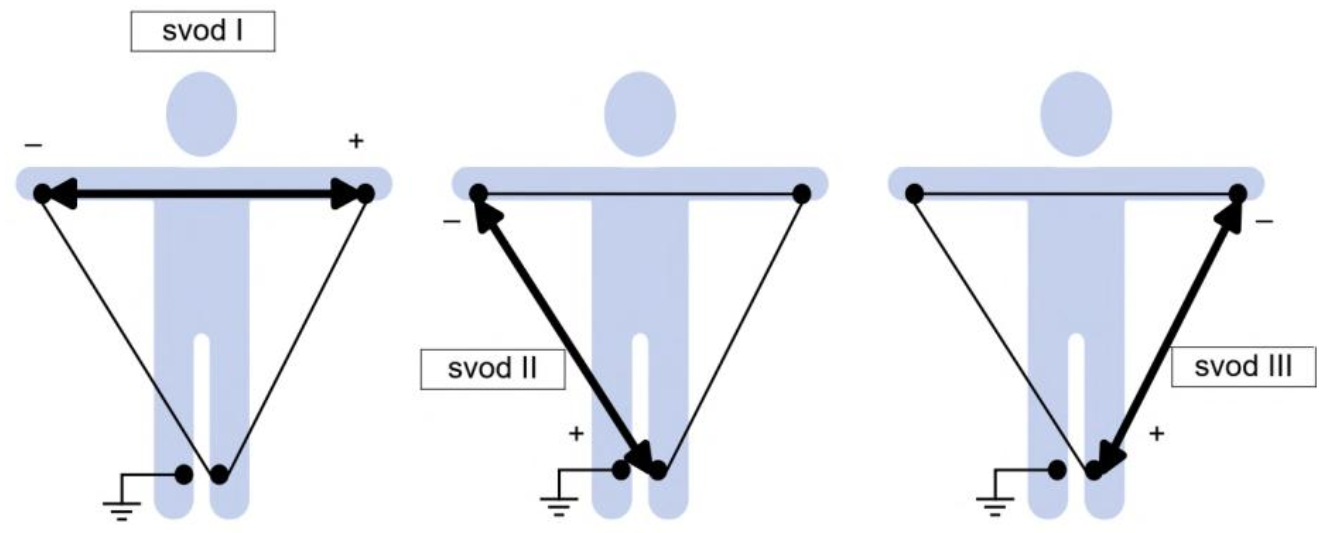
\includegraphics[width=0.7\textwidth]{anatomy/bipolar}
			      \caption{Bipolární končetinové svody~\cite{Kittnar2020}}
			      \label{fig:bipolar}
		      \end{center}
	      \end{figure}
	\item \textbf{Goldbergerovy unipolární končetinové svody (aVR, aVL, aVF)} --
	      původně tvořily spoje aktivních elektrod s Wilsonovou virtuální
	      svorkou. K Wilsonově svorce byly připojeny všechny končetinové svody
	      přes vysoký odpor k zajištění nulového potenciálu na této svorce.
	      Později byl tento způsob upraven Goldbergerem, který touto modifikací
	      zesílil amplitudu svodů na záznamu. Zesílení vzniká odpojením aktivní
	      elektrody od Wilsonovy svorky, čímž je následně měřen potenciál pouze
	      mezi odpojenou elektrodou a zbylými elektrodami~\cite{Kittnar2020}.
	      \begin{figure}[H]
		      \begin{center}
			      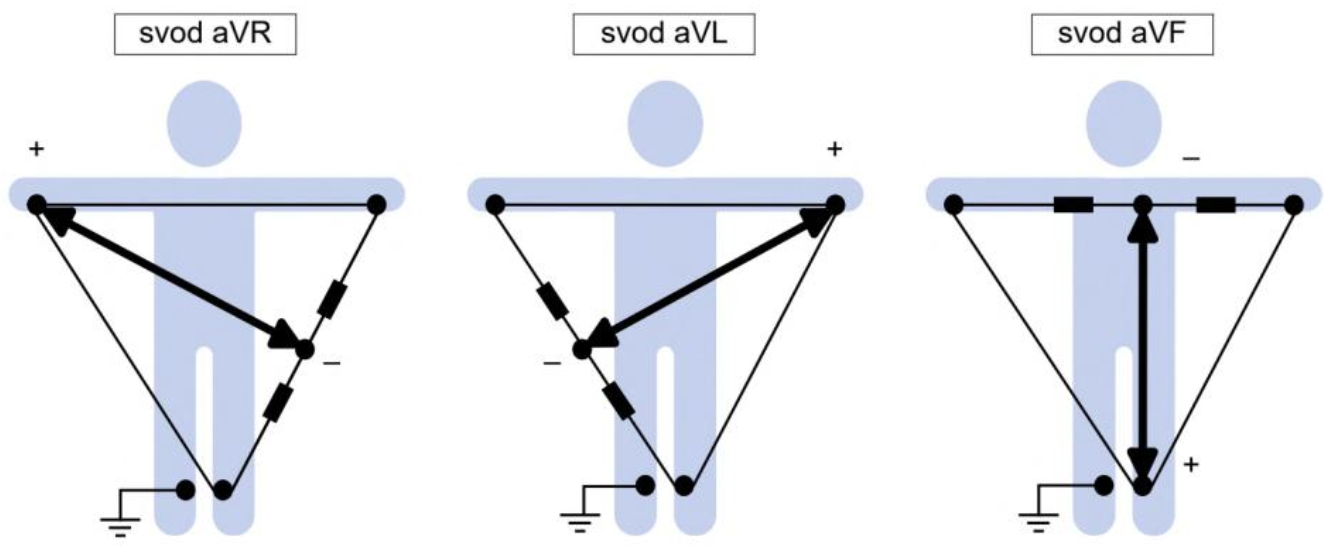
\includegraphics[width=0.7\textwidth]{anatomy/unipolar1}
			      \caption{Unipolární končetinové svody~\cite{Kittnar2020}}
			      \label{fig:unipolar1}
		      \end{center}
	      \end{figure}
	\item \textbf{Wilsonovy unipolární hrudní svody (V1 -- V6)} -- sestávají z
	      šesti hrudních elektrod zapojených proti referenční Wilsonově svorce.
	      Wilsonova nulová svorka je zde opět tvořená spojením končetinových
	      svodů přes odpor. Změnou v tomto zapojení je přechod z frontální
	      roviny měření elektrické aktivity srdce do horizontální. V kombinaci s
	      předešlými Goldbergerovy svody tak vzniká prostorová informace o
	      elektrickém poli myokardu~\cite{Kittnar2020}.
	      \begin{figure}[h]
		      \centering
		      \subcaptionbox{Unipolární hrudní svod~\cite{Kittnar2020}}
		      [.35\linewidth]{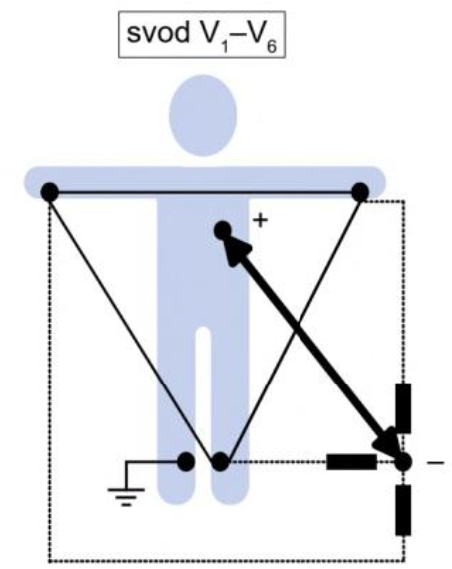
\includegraphics[height=5cm]{anatomy/unipolar2}}
		      \hfill
		      \subcaptionbox{Přiložení unipolárních hrudních svodů podle Wilsona
			      (vlevo) a přiřazení elektrod k srdci v příčném průřezu
			      (vpravo)~\cite{Haberl2012}}
			      [.6\linewidth]{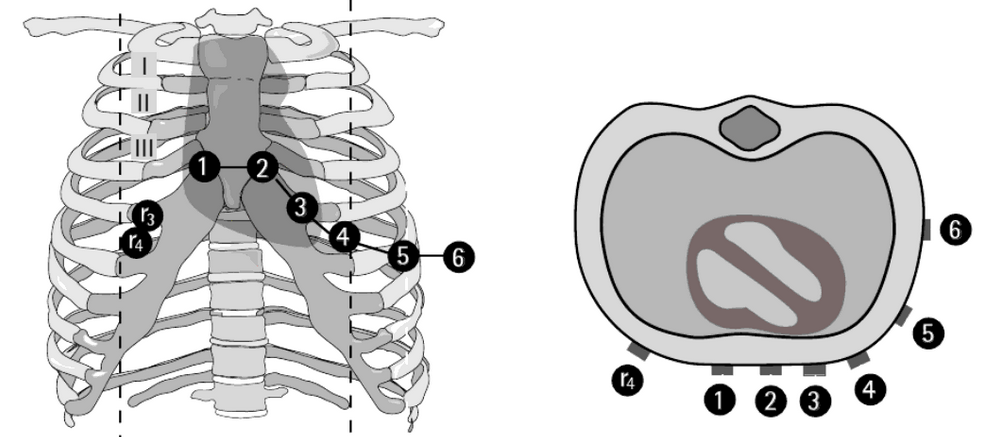
\includegraphics[height=4cm]{anatomy/unipolar3}}
		      \caption{Wilsonovy unipolární hrudní svody}
		      \label{fig:wilson}
	      \end{figure}
\end{enumerate}

Kombinací všech zmíněných svodů vzniká standardní klinický 12-svodový EKG
záznam, který se běžně používá v praxi. Někdy se využívají i další přídavné
svody, jako například etážové, ortogonální nebo jícnové svody. Graficky se
zaznamenává na milimetrový papír nebo je EKG signál vidět na obrazovce v digitalizované
podobě. Délka záznamu se liší v závislosti na diagnostice. K záznamu se používají různé typy EKG přístrojů, které často snímají
více biologických veličin, než pouze elektrickou aktivitu srdce. Mezi přístroje,
které se k měření využívají, se řadí například pacientské monitory vitálních
funkcí, v případě mobilnějšího řešení Holterův monitor (Holter). Holterovo
monitorování se nejčastěji uplatňuje u dlouhodobého kontinuálního záznamu
srdeční aktivity, obvykle 24 hodin, kde je třeba v rámci diagnostiky sledovat
příležitostné srdeční úkazy. Největší výhodou v případě Holterova monitoru je
jeho konstrukce v podobě krabičky. Ta velikostí nepřesahuje mobilní telefon,
díky čemuž je jednoduše přenositelná~\cite{Surawicz2008}.

\subsection{Zpracování záznamu srdeční aktivity}
\label{section:ecg_processing_theory}
Monitorování či analýza EKG tvoří nepostradatelnou část v mnoha diagnostických a
terapeutických případech. Než se ale na výstupu, například v podobě displeje,
objeví EKG křivka či jiné vypočtené parametry, musí se signál
předzpracovat, jinak by tyto parametry byly v praxi zavádějící.

Biologické signály se zpravidla předzpracovávají použitím filtrů. Filtrací
signálu se mění tvar a spektrum původního signálu, čímž dochází k zvýraznění nebo
potlačení jeho specifických složek. V případě EKG signálu se jedná o složky v
jeho frekvenční doméně, reprezentované harmonickými komponenty, které popisují
relace mezi amplitudou a časem~\cite{Jan2002}. Na základě původu a povahy
signálu se filtry dělí na analogové, diskrétní a číslicové (digitální). Navzájem
se mezi sebou liší způsobem provedení náležitých operací~\cite{Skop1994}.
Analogové filtry jsou realizovány v podobě RLC článků, které se skládají z
rezistorů (R), cívek (L) a kondenzátorů (C). Dále se články dělí na pasivní a
aktivní, které využívají zesilovače. Diskrétní a digitální filtry představují
spíše algoritmy než obvody~\cite{Prchal2000}. Jelikož je v této práci především
použita lineární digitální filtrace, bude nadále detailněji rozebrána oblast
diskrétních lineárních časově invariantních systémů (LTI), a to konkrétně
lineární časově invariantní filtry~\cite{Jan2002}.

Před samotnou filtrací se obvykle provádí spektrální analýza signálu neboli
převod signálu z časové domény do frekvenční pomocí rychlé Fourierovy transformace
(FFT), což poskytuje informace o jeho frekvenčním složení~\cite{Prchal2000}.
Díky získané frekvenční charakteristice a znalosti užitečného frekvenčního
rozsahu komponentů EKG signálu a šumu je navržen filtr, který má za úkol
potlačit vliv nežádoucích interferencí. Příklad obecného spektra EKG signálu a
jeho jednotlivých složek lze vidět na Obr.~\ref{fig:ecg_spectrum}. Na obrázku je
znázorněn QRS region ve frekvenčním rozsahu 10--15~\si\Hz,~avšak nejedná se o
pevně daný rozsah. V literatuře se uvádějí různé rozsahy a primárně záleží na
EKG signálu samotném.

\begin{figure}[h]
	\begin{center}
		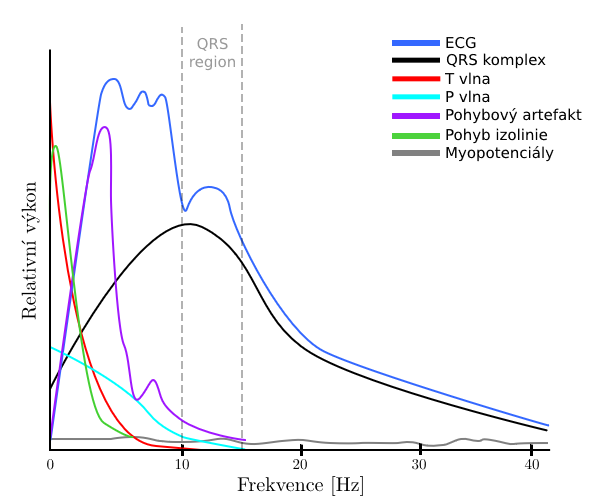
\includegraphics[width=0.7\textwidth]{figures/ecg_spectrum}
		\caption{Spektrum EKG komponentů a artefaktů}
		\label{fig:ecg_spectrum}
	\end{center}
\end{figure}

Digitální filtry se navrhují tak, aby jejich vlastnosti splňovaly nároky, které
jsou obvykle kladeny ve kmitočtové oblasti. Mezi tyto vlastnosti se primárně
řadí amplitudová a fázová charakteristika. Realizace filtru následně probíhá
určením a optimalizací vypočítaných koeficientů společně s jejich počtem tak,
aby se frekvenční charakteristika navrženého filtru co nejvíce přibližovala
požadované frekvenční charakteristice, specifikované realizovatelnou LTI
strukturou. Podle frekvenční charakteristiky se rozlišují 4 základní typy
filtru: dolní propust (DP, lowpass filter), horní propust (HP, highpass filter),
pásmová propust (PP, bandpass filter) a pásmová zádrž (PZ, notch filter). Na
Obr.~\ref{fig:amp_characteristics} jsou ideální amplitudové charakteristiky
nerealizovatelných LTI struktur ($|H_i(\widetilde\omega)|$), kterých se reálné
realizace zmíněných základních filtrů snaží
dosáhnout~\cite{Skop1994,Prchal2000}. V praxi se počítá s jistou tolerancí,
která vyjadřuje kolísání od ideální amplitudové charakteristiky. K zobrazení
tolerancí filtru se používají toleranční diagramy~\cite{Prchal2000,Lyons1997}.

\begin{figure}[h]
	\centering
	\begin{minipage}[b]{0.4\textwidth}
		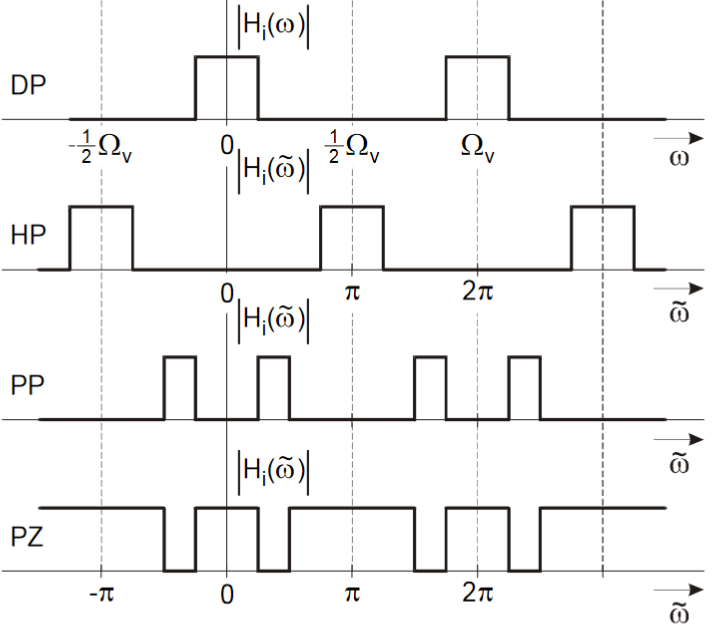
\includegraphics[width=1\linewidth]{figures/amp_characteristics}
		\caption{Ideální amplitudové charakteristiky~\cite{Skop1994}}
		\label{fig:amp_characteristics}
	\end{minipage}
	\hfill
	\begin{minipage}[b]{0.5\textwidth}
		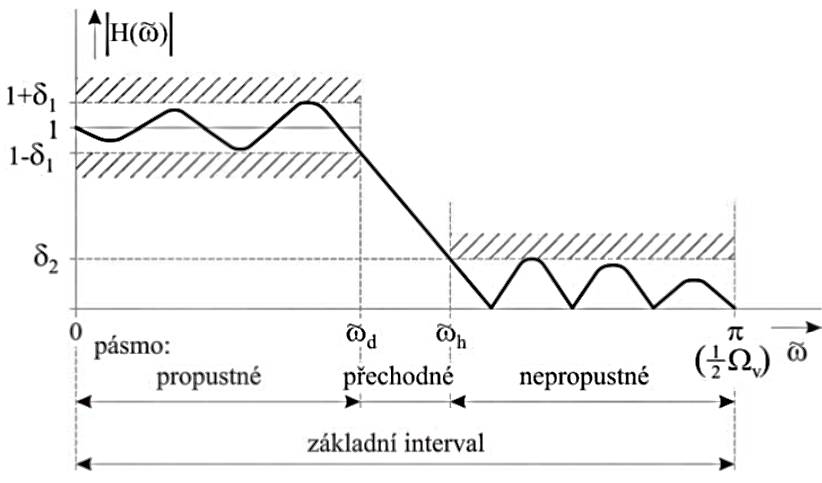
\includegraphics[width=1\linewidth]{figures/tolerance_diagram}
		\caption{Toleranční diagram filtru typu DP~\cite{Skop1994}}
		\label{fig:tolerance_diagram}
	\end{minipage}
\end{figure}

V tolerančním diagramu na Obr.~\ref{fig:tolerance_diagram} jsou znázorněny další
parametry, na které je také třeba dbát při návrhu filtru. Oscilacím, viditelným
v propustném a nepropustném pásmu, se přezdívá vlnění. Parametr \textdelta
\textsubscript{1} (passband ripple), vyjadřuje variaci (zvlnění) amplitudy v
propustném pásmu navrženého filtru a je roven maximální odchylce o jednotkové
velikosti. Parametr \textdelta \textsubscript{2} (stopband attenuation) je
velikost odezvy útlumu, která vyjadřuje maximální ztrátu signálu v nepropustném
pásmu a rovná se maximální odchylce od 0. Frekvence \textomega \textsubscript{d}
a \textomega \textsubscript{h} určují šířku přechodného
pásma~\cite{Prchal2000,Lyons1997}. Přechodové pásmo, zejména jeho sklon, se
odvíjí od složitosti filtru a je jedním z hlavních východisek při posuzování
kvality navrženého filtru~\cite{Jan2002}.

Další důležitou vlastností, ze které se vychází při návrhu digitálních filtrů,
je impulzní odezva. Tato vlastnost dělí digitální filtry na filtry s konečnou
impulzní odezvou (FIR) a nekonečnou impulzní odezvou (IIR)~\cite{Skop1994}.

Použití filtrů s konečnou impulzní odezvou má výhodné uplatnění především tehdy,
když je potřeba lineární fázové charakteristiky. Lineární fáze způsobuje
ekvivalentní fázový posun všech frekvencí v čase, tudíž je zachované stejné
zpoždění signálu na výstupu ve srovnání s vstupním signálem. FIR filtry se dají
navrhnout s přesně lineární fázovou charakteristikou, pokud je jejich impulzní
odezva symetrická nebo asymetrická~\cite{Prchal2000}. Matematická definice
filtru vychází z principu superpozice LTI systémů a je definována jako konečná
diskrétní konvoluce~\cite{Jan2002}:
\begin{equation}
	\label{eq:conv_fir}
	y_n = \sum_{k=1}^{N-1} x_{n-k} h_k
\end{equation}
kde $N$ je řád filtru, $x$ vstupní signál a $h$ je vektor systémových koeficientů
impulzní odezvy filtru pro které platí $h = [h_n],~n \in \langle 0,N-1
\rangle$~\cite{Jan2002}. Stabilita filtrů vychází ze z-transformace impulzní
odezvy~\cite{Jan2002}:
\begin{equation}
	\label{eq:transfer_fir}
	H(z) = \sum_{n=0}^{N-1} h_n z^{-n}
\end{equation}
která je po transformaci ve své rovině dána jen nulovými body~\cite{Jan2002}.
Frekvenční charakteristika filtrů~\cite{Jan2002}:
\begin{equation}
	\label{eq:freq_fir}
	G(\omega) = H(e^{j \omega T}) = \sum_{n=0}^{N-1} h_n e^{-j \omega T}
\end{equation}
je spojitá periodická funkce s periodou $2\pi/T$~\cite{Jan2002}. Jelikož je
frekvenční charakteristika $G(\omega)$ spojená s impulzní odezvou
$h(n)$ Fourierovou transformací~\cite{Prchal2000}, tak koeficienty impulzní
odezvy $h_n$ vycházejí z Fourierovy řady. Díky tomu lze filtry tohoto typu
poměrně snadno navrhnout~\cite{Jan2002}. Další vlastnosti FIR filtrů, které
mohou sloužit jako rozhodovací kritérium při návrhu filtru,
jsou~\cite{Prchal2000}:
\begin{itemize}[noitemsep]
	\item Absolutní stabilita,
	\item Nerekurzivní struktura,
	\item Jednoduchá implementace,
	\item Vysoká výpočetní náročnost.
\end{itemize}

Pokud lineární fázová charakteristika nehraje roli, volí se spíše filtry typu
IIR. Filtry tohoto typu umožňují dosáhnout stejné útlumové charakteristiky jako
u FIR filtrů při menším počtu koeficientů~\cite{Prchal2000}. Výhoda malé
výpočetní náročnosti IIR filtrů má uplatnění primárně ve zpracování signálu v
reálném čase. Další velkou výhodou je široký rozsah realizací, hlavně možnost
návrhu IIR filtru s podobnými charakteristikami analogových
filtrů~\cite{Jan2002,Lyons1997}. Populární biomedicínské IIR implementace
analogových filtrů jsou především Butterworthovy, Čebyševovy (Chebyshev),
Besselovy a Eliptické filtry~\cite{Paarmann2006}. Návrh IIR filtrů je
komplikovanější než u FIR filtrů a často může představovat složitou
optimalizační úlohu. Matematicky jsou IIR filtry definované rekurzivními
diferenčními rovnicemi~\cite{Jan2002}:
\begin{equation}
	\label{eq:conv_iir}
	y_n = \sum_{i=0}^{r} L_i x_{n-i} - \sum_{i=1}^{m} K_i y_{n-i}
\end{equation}
kde $r$ spolu s $L_i$ je řád a koeficienty nerekurzivní části filtru. Naopak $m$
je řád a $K_i$ jsou koeficienty rekurzivní části filtru. Obecně platí $r \leq
m$~\cite{Jan2002,Prchal2000}. Přenosová funkce~\cite{Jan2002}:
\begin{equation}
	\label{eq:transfer_iir}
	H(z) = \frac{\sum_{i=0}^{r} L_i z^{m-i}}{\sum_{i=0}^{m} K_i z^{m-i}} = A \frac{\prod_{i=1}^{r} (z-n_i)}{\prod_{i=1}^{m} (z-p_i)}
\end{equation}
je v z-rovině vyjádřená podílem polynomů, kde $Li$ a $Ki$ jsou systémové
konstanty. Často se lze setkat s následným součinovým vyjádřením, které filtr
popisuje pomocí konfigurace pólů $p_i$, nulových bodů $n_i$ a zesílení
$A$~\cite{Jan2002,Prchal2000}. Vyjádření frekvenční charakteristiky je v případě
IIR filtrů složitější a obvykle se používá k popisu spíše vztah pro amplitudovou
a fázovou charakteristiku~\cite{Jan2002}:
\begin{equation}
	\label{eq:ampphase_iir}
	|G(\omega)| = A \frac{\prod_{i=1}^{r} d_i}{\prod_{i=1}^{m} l_i} ~\text{~a~}~ arg(G(\omega)) = (m-r)\omega T + \sum_{i=1}^{r} \Phi_i - \sum_{i=1}^{m} \Psi_i
\end{equation}
kde $d_i$ spolu s $l_i$ jsou vzdálenosti mezi bodem $e^{j\omega T}$ a nulami
(póly). $\Phi_i$ a $\Psi_i$ jsou úhly náležitých
spojnic~\cite{Prchal2000,Jan2002}. Níže jsou další vybrané vlastnosti IIR
filtrů~\cite{Jan2002}:
\begin{itemize}[noitemsep]
	\item Rekurzivní struktura,
	\item Nízká latence zpracování,
	\item Nelineární fázová charakteristika,
	\item Menší stabilita.
\end{itemize}

\begin{figure}[h]
	\begin{center}
		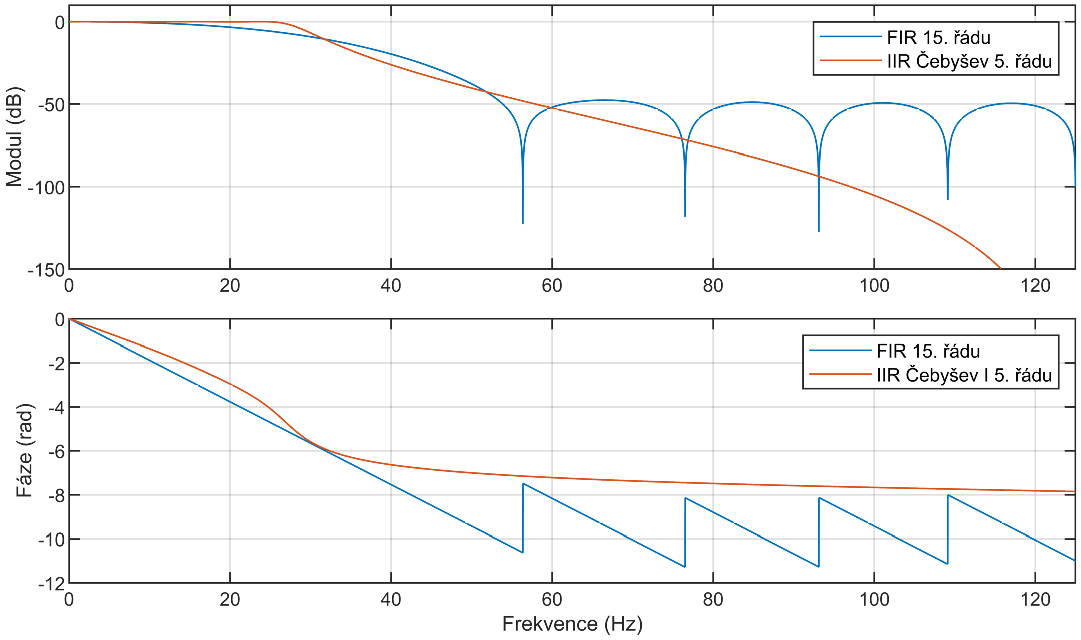
\includegraphics[width=1\textwidth]{figures/filters_comparison}
		\caption{Rozdíl amplitudové a fázové frekvenční charakteristiky FIR a IIR filtru}
		\label{fig:filters_comparison}
	\end{center}
\end{figure}

Rozdíl mezi FIR a IIR filtry je viditelný vzájemným porovnáním jejich impulsní a
frekvenční charakteristiky. Na Obr.~\ref{fig:filters_comparison} jsou graficky
znázorněny tyto charakteristiky pro FIR filtr 15. řádu a Čebyševův filtr 5. řádu
typu I. Filtry byly navrženy jako dolní propust s mezní frekvencí 25~\si\Hz. I
přes značný grafický rozdíl impulsních charakteristik je útlumová úroveň filtrů
velmi podobná, avšak výpočetně IIR filtru stačilo 6 koeficientů oproti FIR
filtru, který jich vyžadoval 15. Hlavní rozdíl vyplývá především z fázové
charakteristiky, kde se v propustném pásmu, a hlavně kolem mezní frekvence
projevuje nelineární fázový charakter IIR filtru.

Včetně lineárních metod filtrace se v praxi často užívají i další metody
předzpracování mezi které se řadí například nelineární a adaptivní
filtrace~\cite{Sornmo1982,Pan1985}, vlnkové
transformace~\cite{Yao2020,Ndiaye2020}, korelační analýza, kumulační metody nebo
neuronové sítě~\cite{Kiranyaz2016,Zhai2018}~\cite{Jan2002}. Po filtraci signálu
a potlačení nežádoucích rušivých složek přichází na řadu jeho segmentace a
extrakce komponentů potřebných k analýze. Na extrahované komponenty se následně
aplikují další postupy hodnotící fyziologické jevy, mezi které nejčastěji patří
HRV.

\subsubsection{Nežádoucí elementy EKG signálu}
\label{section:artifacts_theory}
EKG signál často zkreslují mnohočetné okolní a elektrofyziologické vlivy, které
mohou vést k jeho nesprávné interpretaci. Nejčastější rušivé prvky, které se
projevují na signálu jsou: síťový brum, myopotenciály, pohybové artefakty nebo
špatné umístění elektrod~\cite{Surawicz2008}.

Sítový brum neboli elektrická interference generovaná střídavým proudem z
rozvodné sítě, je jedním z nejběžnějších artefaktů projevujících se v
biologických signálech. Příčinou jeho vzniku může být špatná funkce zařízení nebo
vliv elektromagnetického rušení okolní techniky v blízkosti měřícího přístroje.
Na Obr.~\ref{fig:ac_Interference} je vidět vliv střídavého proudu o frekvenci
50~\si\Hz~na EKG signál~\cite{Goldberger2017}. Nejčastěji se k eliminaci
úzkopásmového rušení tohoto typu volí filtry navržené jako pásmová zádrž, které
nepropouští specifikované frekvence signálu~\cite{Kher2019}.

\begin{figure}[h]
	\begin{subfigure}[b]{0.5\linewidth}
		\centering
		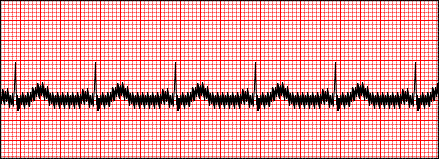
\includegraphics[width=0.8\linewidth]{ecg/ac_Interference}
		\caption{AC rušení}
		\label{fig:ac_Interference}
		\vspace{4ex}
	\end{subfigure}
	\begin{subfigure}[b]{0.5\linewidth}
		\centering
		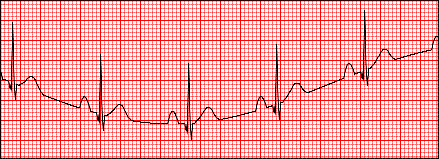
\includegraphics[width=0.8\linewidth]{ecg/w_baseline}
		\caption{Pohyb izoelektrické linie}
		\label{fig:w_baseline}
		\vspace{4ex}
	\end{subfigure}
	\begin{subfigure}[b]{0.5\linewidth}
		\centering
		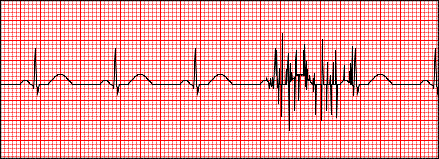
\includegraphics[width=0.8\linewidth]{ecg/muscle_tremor}
		\caption{Myopotenciály (svalový třes, tremor)}
		\label{fig:muscle_tremor}
	\end{subfigure}
	\begin{subfigure}[b]{0.5\linewidth}
		\centering
		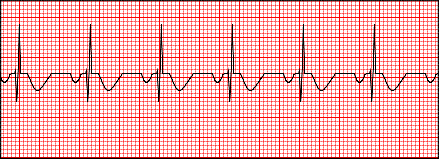
\includegraphics[width=0.8\linewidth]{ecg/rev_electrodes}
		\caption{Nesprávné umístění elektrod}
		\label{fig:rev_electrodes}
	\end{subfigure}
	\caption{Běžné EKG artefakty~\cite{Mauvila2004}}
	\label{fig:common_artifacts}
\end{figure}

Primárně se pohybové artefakty na EKG signálu projevují kolísáním elektrické
izolinie (drift) od její nulové hodnoty jako je tomu na
Obr.~\ref{fig:w_baseline}. Nevznikají pouze pohybem pacienta, ale i
například manipulací měřicími kabely, špatným kontaktem elektrod nebo vlivem
dýchání pacienta~\cite{Goldberger2017}. V lepších případech stačí ke korekci
driftu filtry typu horní propusti. Někdy je potřeba využít například
vlnkových transformací nebo adaptivní filtrace, obzvláště v situacích fyzického
pohybu nebo špatného kontaktu elektrod~\cite{Kher2019}.

Svalové artefakty neboli myopotenciály jsou dalším častým typem rušení
vysokofrekvenčního charakteru, které ovlivňuje EKG signál. Svým způsobem patří
tento typ rušení z části mezi předešlé pohybové artefakty, jelikož mohou vznikat
pohybem pacienta. Tento pohyb může být mimovolný například u osob trpících
Parkinsonovou chorobou, kterou obvykle doprovází svalový třes (tremor) nebo
pulzace arteriální tepny pod elektrodou~\cite{Surawicz2008}. Vlivem pohybů
kosterního svalstva vzniká svalová elektrická aktivita (EMG), která náhodně
interferuje s EKG signálem. Na Obr.~\ref{fig:muscle_tremor} je vidět tato
interference v podobě překrytí QRS komplexu
myopotenciálem~\cite{Goldberger2017}. K potlačení myopotenciálu se často
využívají vyhlazovací filtry nebo například filtry typu dolní propust s
Gaussovou impulsní odezvou~\cite{Kher2019}. Populárním vyhlazovacím digitálním
filtrem je Savitzky–Golay filtr~\cite{Schafer2011}.

V neposlední řadě, spíše než rušení, je častou chybou při záznamu EKG špatné
umístění nebo prohození elektrod. Proto je nutné si pamatovat význam barev
elektrod. Každá barva označuje specifické místo na těle, kam má být elektroda
připevněna. Pokud dojde k prohození, dochází k měření jiného obvykle
neočekávaného potenciálu. Na Obr.~\ref{fig:rev_electrodes} je vidět situace, kdy
došlo k záměně bíle a červené elektrody. Výsledkem je inverze všech vln EKG
křivky (P, Q, R, S, T)~\cite{Goldberger2017,Surawicz2008}.

\subsubsection{Detekce EKG komponentů}
\label{section:components_detection_theory}
Detekce, segmentace a extrakce EKG komponentů, nejčastěji QRS komplexu, je v
posledním století velmi studované téma, které těží z rozvoje výpočetní techniky.
Velkým zlomem byl vznik neuronových sítí a příchod umělé inteligence, která
přinesla v této oblasti nespočet nových řešení, primárně v automatizované
detekci a klasifikaci kardiovaskulárních onemocnění~\cite{Kashou2020}. I
přesto, že softwarové implementace detektorů čim dál častěji nahrazují hardwarová
řešení, tak po hardwarové stránce dochází k rozvoji hlavně v mobilních
zařízeních~\cite{Kohler2002}.

\begin{figure}[h]
	\centering
	\begin{tikzpicture}[node distance=2.5cm, thick, scale=0.84, every node/.style={scale=0.9}]
		\node (pro1) [process, xshift=2cm, text width=2cm] {Lineární filtrace};
		\node (pro2) [process, right of=pro1, xshift=0.8cm, text width=2cm] {Nelineární filtrace};
		\node (Title1) [text=black!50, below of=pro1, node distance=1.2cm, xshift=1.7cm] {Předzpracování};
		\node (blok1) [draw=black!50, dashed, inner sep=0.4cm, fit={(pro1) (pro2) (Title1)}] {};
		\node (start) [left of=blok1, node distance=5cm] {};

		\node (pro3) [process, right of=pro2, xshift=1.8cm, text width=2cm] {Detekční algoritmus};
		\node (pro4) [process, right of=pro3, xshift=0.8cm, text width=2cm] {Rozhodovací pravidlo};
		\node (Title2) [text=black!50, below of=pro3, node distance=1.2cm, xshift=1.7cm] {Rozhodování};
		\node (blok2) [draw=black!50, dashed, inner sep=0.4cm, fit={(pro3) (pro4) (Title2)}] {};
		\node (stop) [right of=blok2, xshift=1.5cm] {};

		\draw [arrow] (start) -- node [above] {EKG} (blok1);
		\draw [arrow] (blok1) -- (blok2);
		\draw [arrow] (blok2) -- (stop);
	\end{tikzpicture}
	\caption{Běžná struktura QRS detektorů~\cite{Kohler2002}}
	\label{fig:qrs_detection}
\end{figure}

Prvním východiskem detekce je oblast analýzy, od které se odvíjí potřebné
komponenty a jejich doména. Oblast může být časová nebo frekvenční. Dalším
krokem je výběr nebo návrh samotné metody pro detekci. Nejčastějším případem v
rámci EKG signálu je detekce QRS komplexu, případně jeho dílčích částí. EKG
signál se následně segmentuje na jednotlivé úseky v závislosti na detekovaných
komplexech~\cite{Canento2012}. Detekční algoritmy zpravidla obsahují další
filtry a matematické operace zvýrazňující QRS komplexy spolu s rozhodovacími
pravidly. Rozhodovací pravidla si lze představit jako podmínky, jejichž splněním
je definován nalezený komponent. Z hlediska principu předzpracování se často
používají například algoritmy založené na~\cite{Kohler2002,Vaneghi2012}:
\begin{itemize}[noitemsep]
	\item \textit{digitální filtraci}~\cite{Sornmo1982,Kesel1997481},
	\item \textit{diferenciaci}~\cite{Tompkins1983,Hamilton1987},
	\item \textit{vlnkové transformaci}~\cite{Yao2020,Ndiaye2020},
	\item \textit{počítání průchodů nulou}~\cite{Kohler2003,Turnip2018},
	\item \textit{Hilbertově transformaci}~\cite{Valluraiah2015, Ouali2020},
	\item \textit{matematické morfologii}~\cite{Li1999,Tadejko2007},
	\item \textit{použití neuronových sítí}~\cite{Kiranyaz2016,Zhai2018}.
\end{itemize}

Většina nově vzniklých metod často čerpá a kombinuje poznatky z těch, které se
postupem času staly konvenčními. Nejznámějším případem takové metody, kterou lze
nazývat konvenční, je Pan-Tompkinsův algoritmus~\cite{Pan1985}.

QRS detekční algoritmus, který navrhl a realizoval Pan-Tompkins v roce 1985, je
doposud jedním z nejpopulárnějších algoritmů v oblasti zpracování EKG signálu.
Navržen byl primárně pro aplikace v reálném čase. Algoritmus má dvě hlavní
části, předzpracování signálu a rozhodovací část. Část předzpracování používá 3
typy filtrů -- pásmová propust, derivační filtr, integrační filtr -- k potlačení
šumu a artefaktů signálu~\cite{Alvarez2013}. Derivační filtr potlačuje vlivy P a
T vln. Integrační filtr, se aplikuje v podobě pohyblivého okna pro vyhlazení
signálu~\cite{Pan1985}.
\begin{figure}[h]
	\centering
	\begin{tikzpicture}[node distance=2.5cm, thick, scale=0.85, every node/.style={scale=0.85}]
		\node (start) [startstop] {Vstupní EKG signál};
		\node (pro1) [process, below of=start, yshift=1cm] {Pásmová propust};
		\node (pro2) [process, right of=pro1, xshift=2cm] {Derivační filtr};
		\node (pro3) [process, right of=pro2, xshift=2cm] {Umocnění signálu};
		\node (pro4) [process, right of=pro3, xshift=2cm] {Integrační filtr};
		\node (pro5) [process, below of=pro4, text width=3cm] {Počáteční detekce R vln};
		\node (pro6) [process, below of=pro3, text width=3cm] {Adaptivní prahování};
		\node (pro7) [process, below of=pro2, text width=3cm] {Rozhodovací pravidlo};
		\node (stop) [startstop, below of=pro1] {QRS komplex};

		\draw [arrow] (start) -- (pro1);
		\draw [arrow] (pro1) -- (pro2);
		\draw [arrow] (pro2) -- (pro3);
		\draw [arrow] (pro3) -- (pro4);
		\draw [arrow] (pro4) -- (pro5);
		\draw [arrow] (pro5) -- (pro6);
		\draw [arrow] (pro6) -- (pro7);
		\draw [arrow] (pro7) -- (stop);
	\end{tikzpicture}
	\caption{Pan-Tompkinsův algoritmus}
	\label{fig:pan_tompkins}
\end{figure}
Rozhodovací část neboli část zpracování, se věnuje
detekci QRS komplexů. Pro zvýšení spolehlivosti algoritmu probíhá detekce
zároveň na derivovaném a na vyhlazeném signálu. Prvotním krokem je nalezení
lokálních maxim v podobě R vln. Následně se aplikuje adaptivní prahování formou
pohyblivého okna, pří kterém jsou rozhodovacím pravidlem vybrané pouze R vlny
překračující prahovou hodnotu. Vybrané R vlny představují referenční body
detekovaných QRS komplexů~\cite{Pan1985,Alvarez2013}.

Existuje mnoho dalších QRS detektorů, jejichž řešení se orientuje především
povahou dat a způsobem zpracování. Způsobem zpracování se rozumí, zdali detekce
probíhá na již naměřených datech -- offline -- nebo v reálném čase -- online.
Povaha dat je dána způsobem měření. Záznamy srdeční aktivity naměřené
intrakardiálně nejsou zatížené artefakty tolik jako záznamy pořízené
Holterovským monitorováním. Z toho vyplývá i komplexita detektoru, jelikož EKG
záznamy zatížené mnohočetnými artefakty vyžadují mnohem sofistikovanější
detekční algoritmy. Další populární QRS detektory a jejich srovnání je rozebrané
v~\cite{Kohler2002,Canento2012,Vaneghi2012,Alvarez2013,Karpagachelvi2010}.

\subsection{Variabilita srdeční frekvence}
\label{section:hrv}
Jednou z nejčastěji sledovaných elektrofyziologických veličin je srdeční rytmus.
Je to veličina měnící se s každým dalším úderem srdce, ovlivňována aktivitou
ANS. Jelikož srdeční rytmus vychází normálně ze sinoatriálního uzlu, jedná se o
sinusový rytmus závislý na tonu sympatiku a parasympatiku. Proto se mezi faktory
ovlivňující srdeční rytmus řadí vnější a vnitřní vlivy jako vznik ischemie,
metabolická dysbalance nebo zvýšená kognitivní, emoční a fyzická zátěž, které
jsou zároveň stěžejními pro rozbor samotného EKG záznamu~\cite{Pumprla2014}.
Blíže jsou tyto vztahy popsané v sekci~\ref{section:hr_regulation}. Autonomní
procesy regulující srdeční činnost nebo jiné aktivity podmíněné fyziologickými a
psychofyziologickými vlivy se včetně změny rychlosti srdečního rytmu promítají
jako časové variace mezi jednotlivými stahy srdce. Časové variace neboli lišící
se délky jednotlivých R-R intervalů se obecně označují jako variabilita
srdečního rytmu~\cite{Pumprla2014,Rajendra2007}.

Z HRV vycházejí i další parametry, které se využívají k jejímu hodnocení.
Výpočet a smysl specifických parametrů už spadá pod jednotlivé metody hodnocení
HRV v následující kapitole. K tomu aby bylo možné HRV kvantitativně hodnotit je
potřeba z EKG signálu extrahovat R vlny, jejichž časová diference je právě
hledanou variabilitou. Artefakty EKG mohou v případě HRV analýzy hrát stěžejní
roli pokud došlo k zániku nebo významnému zkreslení některých R vln. Nejčastěji
se u zaniklých R vln používají metody lineární interpolace, které zachovávají
správnou variabilitu. Srovnání rozdílných metod interpolace, včetně té lineární
a dopad chybějících R vln na HRV analýzu již bylo popsané
v~\cite{Kim2007,Peltola2012,Morelli2019}. Další častou příčinou abnormálních R
vln, se kterou se lze v praxi setkat, jsou ektopické stahy. Proto existuje mnoho
algoritmů, které se věnují zpracování R-R intervalů aby bylo možné HRV
hodnotit~\cite{Lipponen2019}.

\subsubsection{Metody hodnocení HRV}
\label{section:hrv_methods}
Hodnocení variability srdečního rytmu neboli zkoumání variace mezi jednotlivými
srdečními stahy nachází dnes velké uplatnění v diagnostice, například v rámci
rychlého neinvazivního zhodnocení kardiovaskulární autonomní regulace.
Nejčastější a základní neinvazivní metody hodnocení HRV mohou být sjednoceny do
časové a frekvenční oblasti, ale existují i další geometrické a nelineární
postupy. Nejzákladnější běžná metoda je spektrální analýza variability srdečního
rytmu, která umožňuje zaznamenat a deklarovat vlivy kardiálního autonomního
nervového systému~\cite{Pumprla2014}. Často se lze setkat, primárně u hodnocení
dlouhodobých EKG záznamů, se statistickou analýzou, která využívá parametry
vypočítané z HRV v časové doméně. Hodnoty jednotlivých parametrů následně slouží
jako indikátory změn pro různé oblasti kardiovaskulárního systému a
ANS~\cite{Malik1996}. Časové a frekvenční metody mají však své technické omezení, 
jako například předpoklad linearity dat a v některých případech se neumějí
vypořádat s interferencemi způsobené ektopickým rytmem~\cite{Hsu2012}. Další
populární geometrickou nelineární metodou je analýza Poincarého grafu, na kterém
je každý R-R interval vynesen proti nadcházejícímu R-R intervalu. 

\begin{figure}[h]
	\begin{center}
		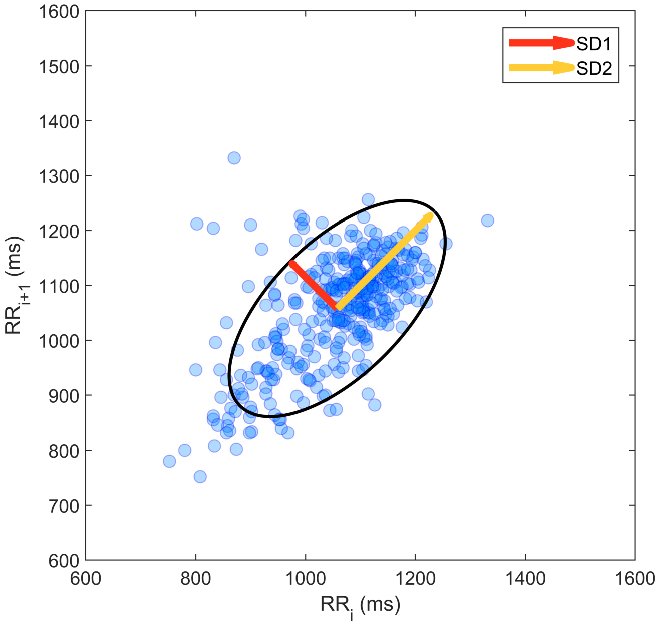
\includegraphics[width=0.6\textwidth]{assets/figures/my_poincare}
		\caption{Poincarého graf}
		\label{fig:wiki_poincare}
	\end{center}
\end{figure}

Poincarého graf (plot, mapa) lze interpretovat jako kartézský souřadnicový systém
tvořící mapu bodů, kde každý bod je definován dvojicí $RR_i$ (osa x) a
$RR_{i+1}$ (osa y)~\cite{Hsu2012,Hejjel2001}. Na rozdíl od předešlých metod se
Poincarého graf vyhodnocuje jak kvalitativně, pomocí tvaru (vzoru) vzniklého z
bodů, tak i kvantitativně, výpočtem SD indexů grafu, které poskytují podobné
informace jako LF a HF složky spektrálního výkonu nebo statistické parametry
SDNN a RMSSD. Z grafu tak lze získat souhrnné i detailní informace o dynamickém
chování srdečního rytmu~\cite{Hsu2012,Kubickova2016}. 

Jak již bylo zmíněno, kvalitativní analýza se orientuje rozložením bodů na
Poincarého grafu a vypovídá o variabilitě. Čím menší je plocha vzoru bodů, tím
menší je variabilita, a naopak. Disperze bodů podél osy grafu procházející
počátkem vypovídá a dlouhodobě variabilitě a rozptýlení bodu kolmo na tuto osu o
krátkodobé. Průnikem diagonálních os grafu je průměrná hodnota R-R
intervalů~\cite{Hejjel2001}. Poloha shluku bodů na diagonále procházející
počátkem hraje také roli. Pozice shluku blíže počátku indikuje vliv sympatiku
zatímco pozice dál směrem na opačnou stranu vliv parasympatiku. Pokud se v grafu
nachází více shluků lze očekávat arytmie. Asymetrie vzoru bodů může vypovídat o
poruchách srdečního rytmu~\cite{Habib2013}. Vizuální charakteristiky Poincarého
grafu se dají vyjádřit i kvantitativně. Nejpopulárnější technikou
kvantitativního hodnocení Poincarého mapy je proložení bodů v grafu elipsou.
Z hlavní a vedlejší osy elipsy lze vypočítat indexy SD1 a SD2. Tvarové
vlastnosti elipsy jsou v souladu vlastnosti tvaru shluku bodů.
SD indexy jsou směrodatné odchylky okamžité variability ve směru
osy~\cite{Habib2013,Mazhar2007}.

Všechny metody jsou pak v praxi využitelné pro včasné odhalení
kardiovaskulárních onemocnění, nicméně jsou použitelné pouze ve specifických
laboratorních podmínkách a jako jiné jsou ovlivnitelné právě fyzickými a
psychologickými faktory~\cite{Habib2013,Kubickova2016}. Parametry HRV můžou
sloužit pro predikci kognitivní zátěže, ale pro jejich spolehlivé určení je
nezbytný pečlivý výběr vhodných metod předzpracování signálu.

\subsubsection{Model neuroviscerální integrace}
Model neuroviscerální integrace popisuje vztahy v rámci periferní
psychofyziologie, neurověd a autonomních funkci spjatých s regulací vagálního
tonu. Znalosti a vztahy těchto oborů jsou kombinované do několika detailně popsaných
teoretických vrstev, dohromady tvořících jediný framework sloužící také jako
prediktivní model, který pak usnadňuje vyhodnotit souvislosti a důsledky
zásadních fyziologických změn srdeční aktivity či veličin s ní
spojených~\cite{Smith2017}.

\begin{figure}[h]
	\begin{center}
		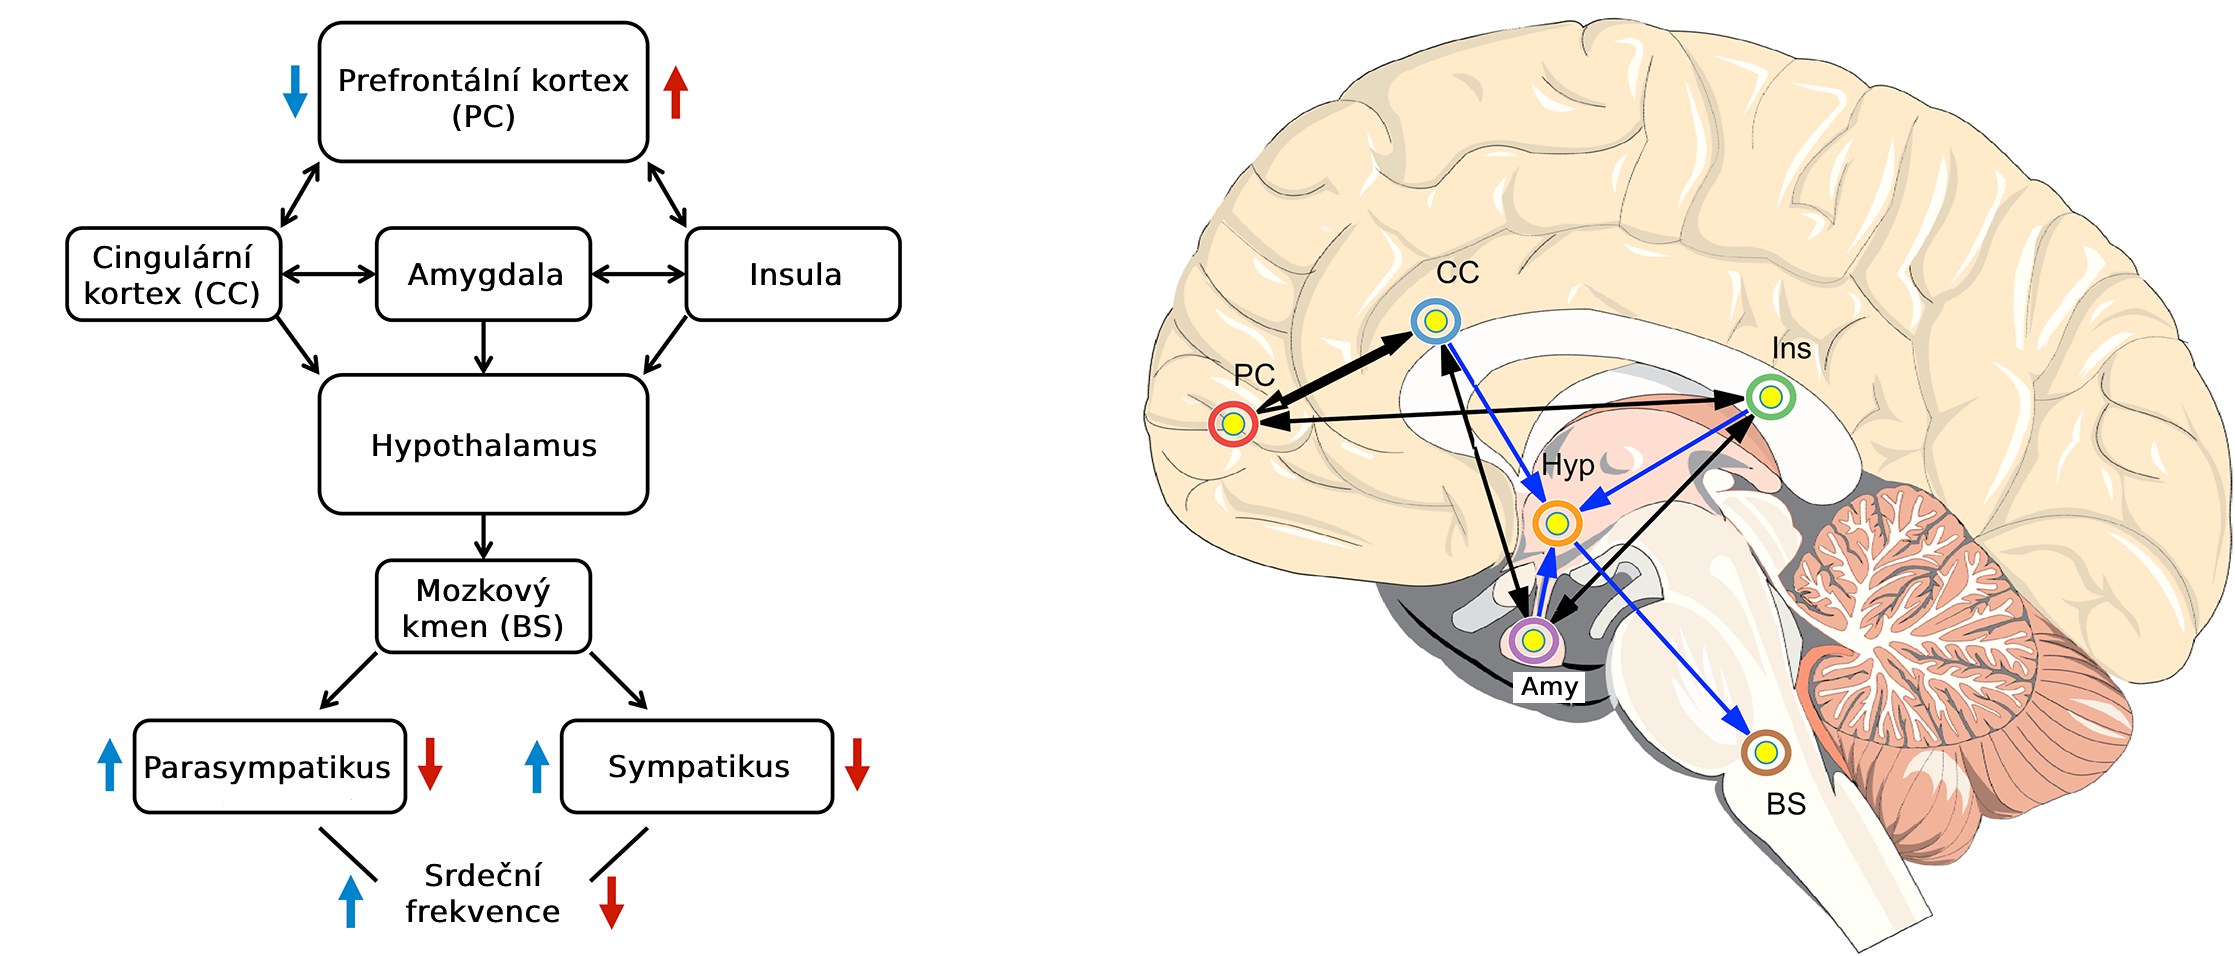
\includegraphics[width=1\textwidth]{diagrams/nvi}
		\caption{Zjednodušený model neuroviscerální integrace (Upraveno a převzato z~\cite{NVI20017})}
		\label{fig:nvi_model}
	\end{center}
\end{figure}

Souvislosti modelu NVI mají například za následek, že odlišné druhy kognitivní
zátěže se promítají do časové a frekvenční domény EKG signálu. Specificky se
projevují jako kvantitativní lineární a nelineární časové parametry nebo velmi
nízko, nízko a vysoko frekvenční složky (VLF, LF, HF) výkonového spektra.
Jednotlivé komponenty slouží pří samotné analýze jako indikátory činnosti
vegetativní nervové soustavy (VNS). Aby bylo ale možné tyto komponenty získat a
porovnávat či jakkoliv hodnotit srdeční aktivitu, musí být záznam srdeční
aktivity patřičně zpracován. Model NVI je nad rámec této práce a detailněji je
rozebrán v~\cite{Smith2017}.

\subsubsection{HRV v diagnostice a terapii}
Dříve panovalo obecné přesvědčení že variace v srdečním rytmu jsou patologický
úkaz a nebylo jim věnované žádné zvláštní pozornosti. Falešná domněnka o HRV
byla poprvé vyvrácena v roce 1978, klinickou studií~\cite{Wolf1978}, která
potvrzuje korelaci snížené HRV s úmrtností a arytmickými komplikacemi během
postinfarktového období. Od té doby se studie na téma nepravidelností sinusového
rytmu začaly rozvíjet. V současnosti je HRV klinicky významnou a
velmi využívanou biometrikou napříč obory. Na Obr.~\ref{fig:hrv_infarct} lze
vidět vývoj HRV během 24h Holterovského monitorování dvou pacientů (D, S) v
postinfarktovém období, konkrétně 7. den po infarktu myokardu. U pacienta $D$
lze pozorovat nekomplikovaný postinfarktový průběh v podobě konstantního vývoje
R-R intervalů. Pacient $S$ umřel 27. den po infarktu~\cite{Malik1990}. Další
rizikové faktory korelující s HRV parametry lze najít v
tabulce~\ref{tab:hrv_factors}.

\begin{figure}[h]
	\begin{center}
		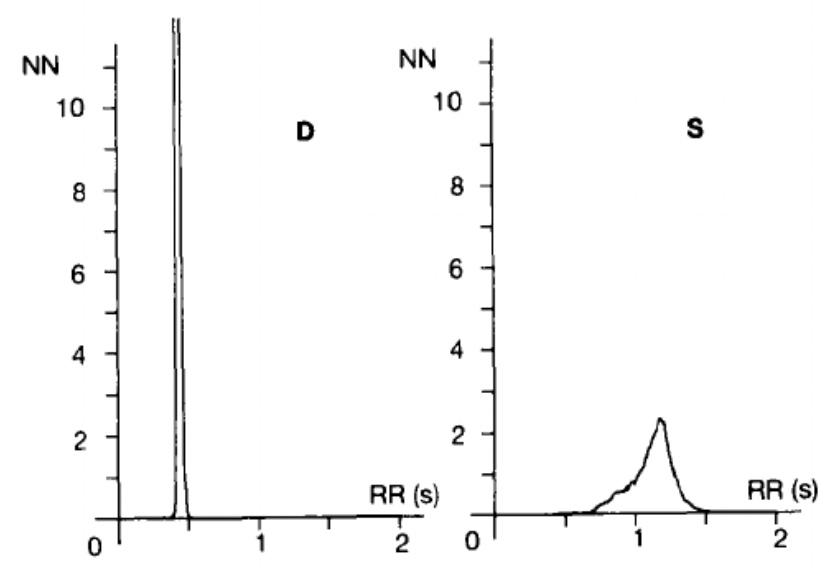
\includegraphics[width=0.5\textwidth]{figures/hrv_infarct}
		\caption{Rozdíly v HRV mezi pacienty (S, D) s vysokým a nízkým rizikem úmrtí v
			postinfarktovém období \cite{Malik1990}}
		\label{fig:hrv_infarct}
	\end{center}
\end{figure}

Ačkoli hodnocení HRV našlo pochopitelně největší praktické uplatnění v oboru
kardiologie, existují další obory, do kterých vnesla tato biometrika v
posledních letech mnoho nových a zásadních poznatků. Jedním z takových oborů je psychologie
a kognitivní psychologie v rámci neuropsychofyziologických vlivů, které jsou
důsledkem změn a procesů probíhajících v ANS~\cite{Bernardi2009}. Tak byla
zformulovaná kognitivní teorie v~\cite{Forte2019,Plass2010}. Studie v rámci
kognitivní
psychologie~\cite{Bernardi2009,Solhjoo2019,Salahuddin2007,Ishaque2020}
potvrzují, že různé druhy kognitivní zátěže ovliňují kardiovaskulární systém,
primárně HRV, a to i z hlediska dlouhodobých korelací se statistickými HRV
parametry. Proto je možné v tabulce~\ref{tab:hrv_factors} vidět faktor typu
pracovního stresu, který se řadí mezi specifický druh kognitivní zátěže.

Prognostický význam má HRV i v řadě dalších klinických a intenzivistických oborů
mezi které například patří diabetologie, renologie a neurologie. S využitím HRV
se lze dále setkat na jednotkách intenzivní péče, kde monitorování této metriky
slouží k predikci potenciálních pooperačních komplikací. Své uplatnění našla i
ve farmakokinetice při posuzování odezvy organismu na podané
léčiva~\cite{Pumprla2014}.

\begin{table}[h]
	\captionsetup{skip=0.5pt}
	\catcode`\-=12
	\scriptsize
	\begin{center}
		\caption[HRV a rizikové faktory]{Vybrané vztahy mezi HRV parametry a
			rizikovými faktory \\ (Upraveno a převzato z \cite{Pumprla2014,Thayer2009})}
		\label{tab:hrv_factors}
		\vspace{1ex}
		\renewcommand{\arraystretch}{1.3}
		\begin{tabular}{|p{1.3cm}|p{1.7cm}|p{4.5cm}|p{5.5cm}|}
			\noalign{\hrule height 2pt}
			\textbf{Riziko} & \textbf{Autor}     & \textbf{Sledovaný parametr a populace}                                  & \textbf{Závěr}                                                                                                                                                                                  \\ \hline
			Hypertenze      & Schroeder          & HRV, hypertenze, krevní tlak. n=11061, 28\% incidence hypertenze        & 1,1–-1,6x riziko rozvoje hypertenze u subjektů s patologickými hodnotami časové analýzy HRV (SDNN, RMSSD, délka R-R int.)                                                                       \\ \hline
			Cholesterol     & Christensen        & HRV a cholesterol. n=85, 55\% s ICHS                                    & Asociace mezi nižší HRV (časová analýza, SDNN, RMSSD) a vyšším cholesterolem u pacientů s ICHS i u zdravých jedinců                                                                             \\ \hline
			Diabetes        & Liao (ARIC studie) & HRV, diabetes, glykemie, inzulinemie. n=1933, 8\% diabetiků             & Snížený výkon v HF pásmu u diabetiků ve srovnání s nediabetiky (p=0,01)                                                                                                                         \\ \hline
			Pohyb           & Sloan              & HRV, aerobní aktivita. n=149 zdravých                                   & Zvýšení SDNN a HF výkonu po 12 týdenním aerobním tréninku. Opětný pokles SDNN a HF výkonu za 4 týdny po ukončení vytrvalostního tréninku                                                        \\ \hline
			Kouření         & Hayano             & HRV, krátko a dlouhodobý efekt kouření. n=81 mužů, 69\% kuřáci          & Pokles HF výkonu již po 1 cigaretě (p=0,006). Zvýšení CCV v LF pásmu za 10–-17 min po kouření (p=0,0001). Nižší CCV v HF pásmu u těžkých kuřáků ve srovnání s nekuřáky/lehkými kuřáky (p=0,008) \\ \hline
			Pracovní stres  & van Amelsvoort     & HRV, pracovní zátěž, fyzická aktivita, pracovní směny. n=135, 84\% mužů & SDNNi během spánku: 69.3 ms proti 85.8 ms, p < 0.05, směna a denní pracovníci                                                                                                                   \\ \noalign{\hrule height 2pt}
		\end{tabular}
	\end{center}
\end{table}
\clearpage

\section{Cíle práce}
Hlavním cílem bakalářské práce je navržení a realizace adaptivního řešení pro
offline zpracování a hodnocení záznamu srdeční aktivity v programovém prostředí
MATLAB.
\clearpage

\section{Metody}
V této kapitole jsou popsány metody použité v bakalářské práci. V
podkapitole~\ref{section:measurement} je rozebrán postup měření EKG záznamů a
použité zařízení. V kapitole~\ref{section:study} je charakterizována kontrolní
skupina probandů a sledované veličiny. V
kapitolách~\ref{section:offline_processing} a~\ref{section:online_processing} je
řešena metodologie online a offline zpracování a hodnocení EKG signálu.
Kapitola~\ref{section:statistical_methods} pojednává o statistickém zpracování
výsledků.

\subsection{Měření EKG signálů}
\label{section:measurement}
Pro účely zpracování a analýzy EKG signálu, které jsou náplní této bakalářské
práce, bylo provedeno pilotní měření krátkodobých záznamů srdeční aktivity na 5
probandech. Postup měření je specifikován v
kapitole~\ref{section:measurement_methodology}. Měřící zařízení je popsané v
následující kapitole.

\subsubsection{Měřící zařízení}
\label{section:measurement_device}
Zařízení použité k měření srdeční aktivity byl Holterův monitor (viz
Obr.~\ref{fig:device}), zajištěný vědeckým týmem Biomechaniky a asistivních
technologií. Skládá se ze dvou komponent: samotné zařízení a 3-svodový EKG kabel
s 3.5~\si\mm~jack konektorem. Vzorkovací frekvence zařízení je 500~\si\Hz.

Přenos dat ze zařízení probíhá bezdrátově na lokální sítí (WLAN), ke které je
třeba zařízení připojit pomocí volně dostupné mobilní aplikace \textit{ESPTouch:
SmartConfig}~\cite{ESPAPP} podle postupu níže. \textit{ESP-TOUCH} je protokol, umožňující
vestavěným systémům (embedded systémy) jednoduché připojení k Wi-Fi sítím pomocí
chytrých mobilních zařízení~\cite{esptouch}. K záznamu dat byla použita
aplikace, naprogramovaná v rámci této práce, jménem \textit{BBPM (Better bpm)},
která se zařízením komunikuje přes protokol \textit{Modbus}~\cite{modbus}.
Aplikace \textit{BBPM} je detailněji popsána v
kapitole~\ref{section:offline_processing}.

\begin{figure}[H]
    \begin{center}
        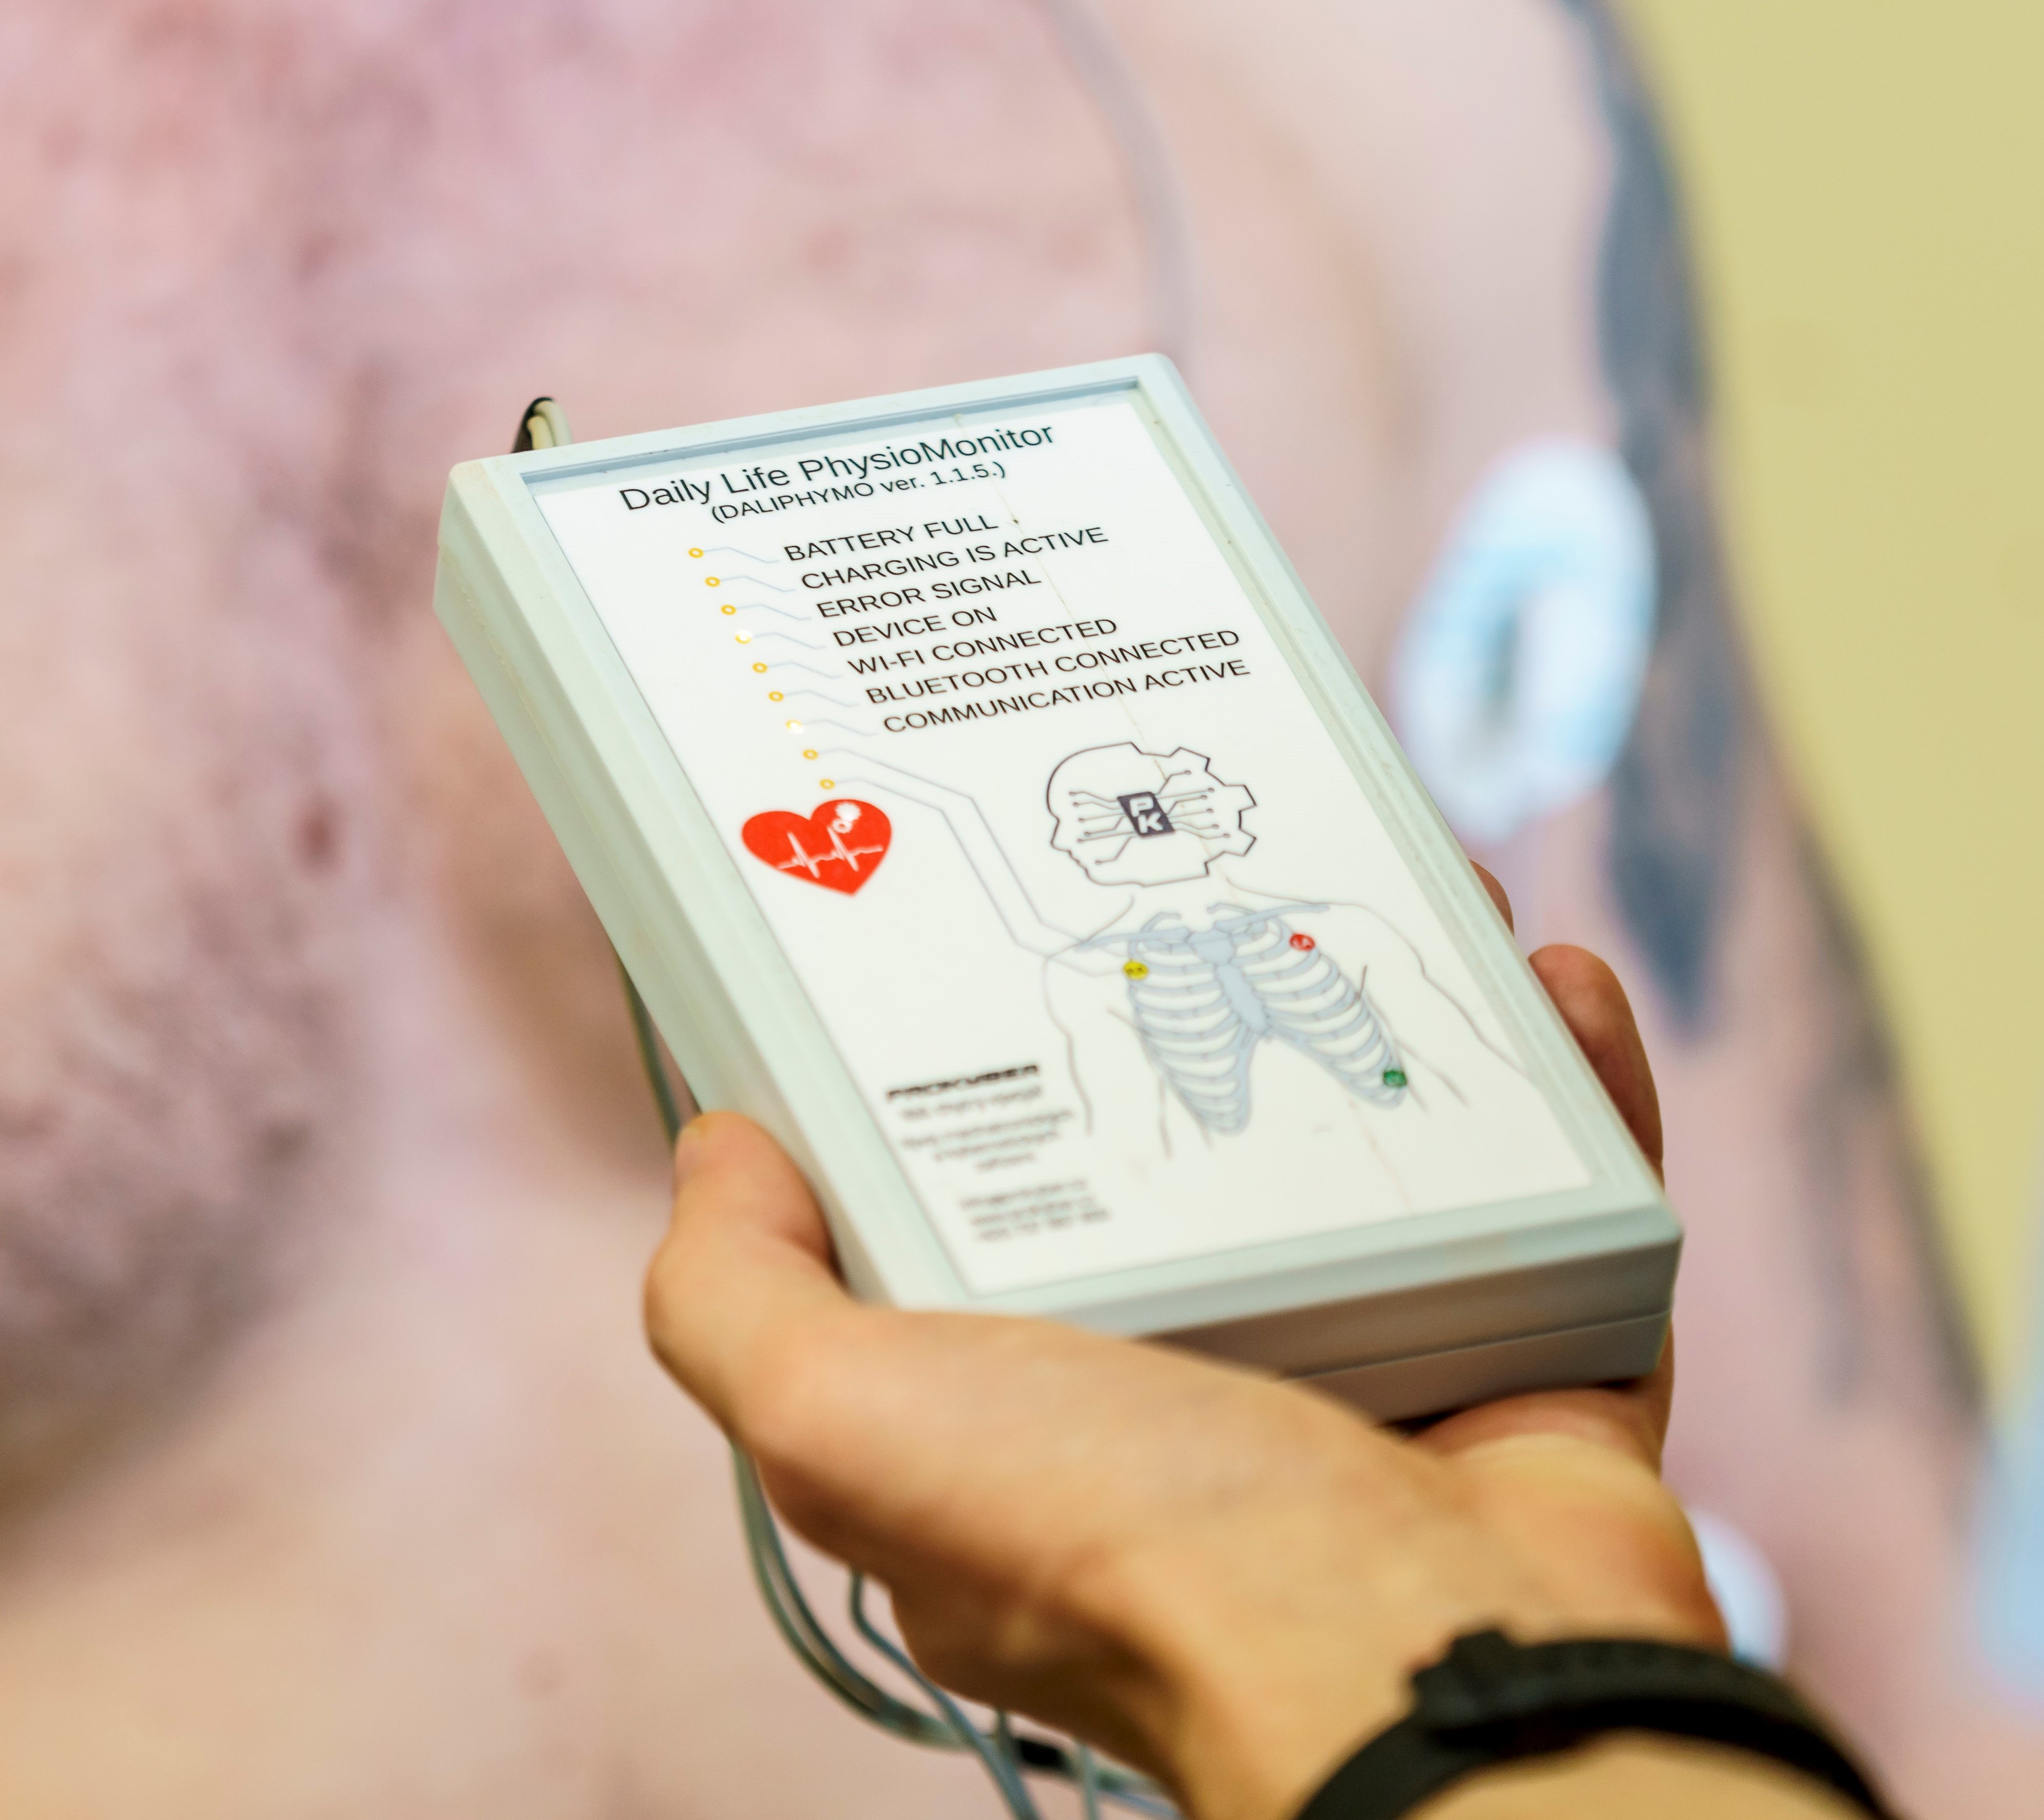
\includegraphics[width=0.9\textwidth]{device/holter1}
        \caption{Měřící zařízení s příslušenstvím}
        \label{fig:device}
    \end{center}
\end{figure}

Holterův monitor musí být při připojování k bezdrátové sítí v bezprostřední
blízkosti chytrého zařízení, kterým bude konfigurován. Postup pro připojení
měřícího zařízení k WLAN sítí je následující:
\begin{enumerate}
    \item Připojení chytrého mobilního zařízení, které bude sloužit ke
          konfiguraci Holterova monitoru, k požadované WLAN sítí, kde bude
          probíhat komunikace.
    \item Přepnutí měřícího zařízení do režimu konfigurace stiskem tlačítka
          \textbf{Config}, které se nachází na horní ploše okraje zařízení.
    \item Spuštění aplikace \textit{ESPTouch: SmartConfig}.
    \item Ověření správně vybrané WLAN sítě pomocí identifikátoru \textbf{SSID}
          v horní části úvodní obrazovky aplikace (Obr.~\ref{fig:app_screen1}).
    \item Vyplnění hesla v kolonce \textbf{Password} náležícího zvolené WLAN
          sítí. Ostatní parametry jsou ponechány ve výchozím stavu.
    \item Stisk tlačítka \textbf{Confirm} v dolní části aplikace pro zahájení
          konfigurace a připojení Holterova monitoru k vybrané sítí.
\end{enumerate}

Pokud se měřící zařízení připojilo úspěšně k vybrané WLAN sítí, objeví se
notifikace jako na Obr. \ref{fig:app_screen2} a zároveň je navázané spojení
indikované rozsvícenou LED kontrolkou na předním panelu Holterova monitoru u položky
\textbf{WI-FI CONNECTED}. Při nezdařeném pokusu připojení je nutné opakovat
kroky od bodu 2 nebo případně zkontrolovat stav baterie Holterova monitoru.

\begin{figure}[h]
    \centering
    \begin{subfigure}[b]{0.45\textwidth}
        \centering
        \textcolor{cyan}{\fboxrule=1.5pt\fboxsep=0pt\fbox{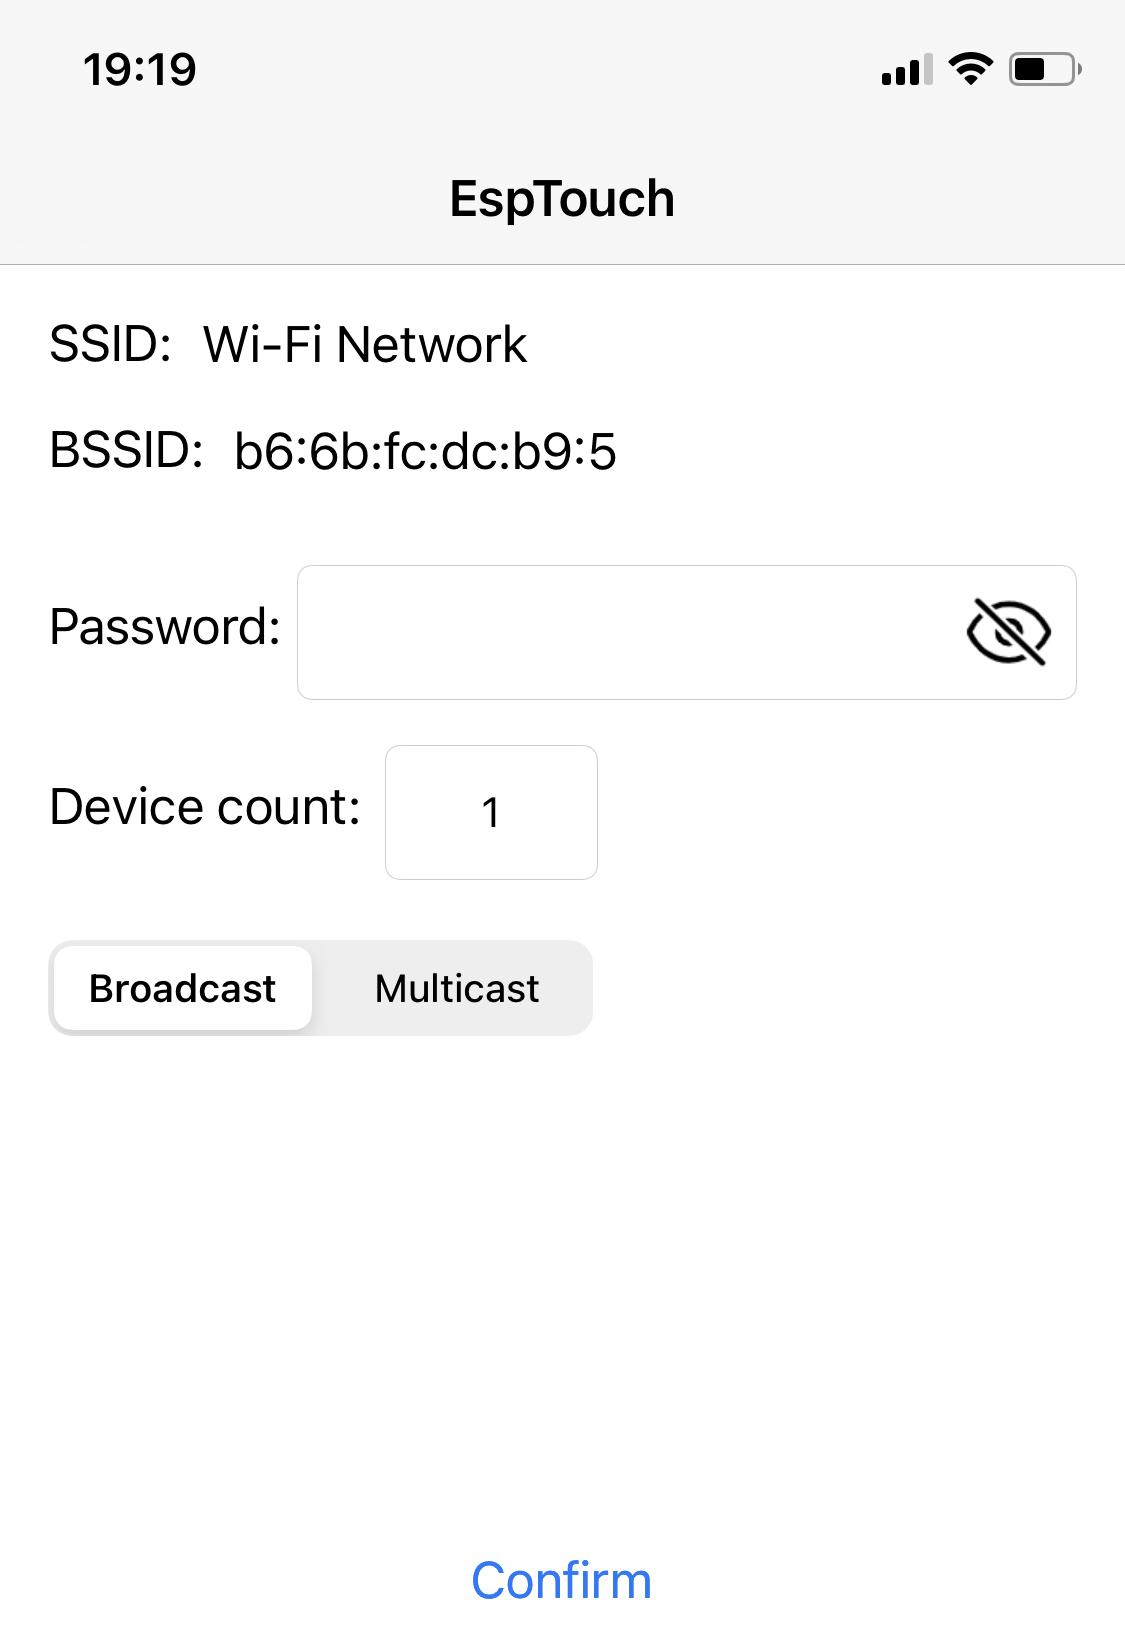
\includegraphics[width=0.8\linewidth]{device/app_screen1}}}
        \caption{Úvodní obrazovka aplikace}
        \label{fig:app_screen1}
    \end{subfigure}
    \hfill
    \begin{subfigure}[b]{0.45\textwidth}
        \centering
        \textcolor{cyan}{\fboxrule=1.5pt\fboxsep=0pt\fbox{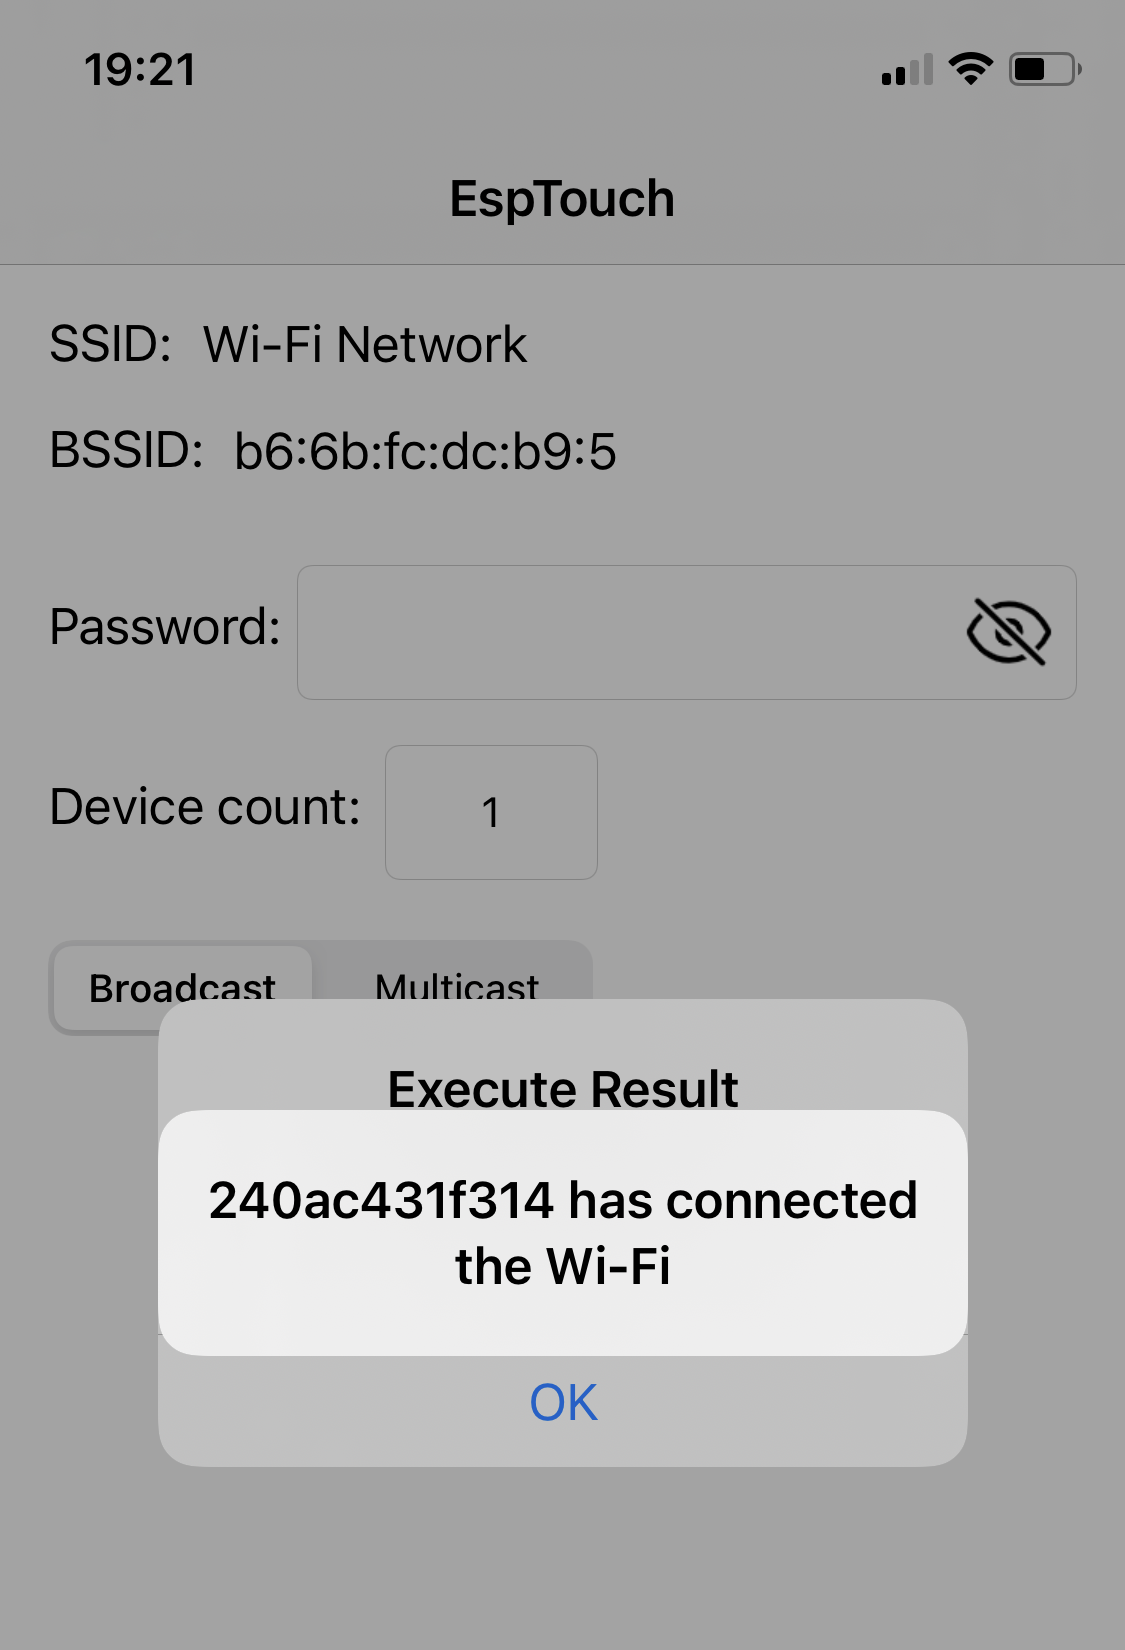
\includegraphics[width=0.8\linewidth]{device/app_screen2}}}
        \caption{Notifikace úspěšného připojení}
        \label{fig:app_screen2}
    \end{subfigure}
    \caption{Konfigurace měřícího zařízení v aplikaci \textit{ESPTouch:
            SmartConfig}~\cite{ESPAPP}}
    \label{fig:esptouch_app}
\end{figure}

\subsubsection{Metodika měření}
\label{section:measurement_methodology}
Metodika měření spočívá v krátkodobém záznamu srdeční aktivity ve dvou odlišných
situacích. Před měřením je na subjekt připojeno měřící zařízení, popsané v
sekci~\ref{section:measurement_device}, pomocí adhezivních EKG elektrod (viz
Obr.~\ref{fig:device_usage}). Jedná se o bipolární hrudní 3-svodové zapojení
elektrod (viz kapitola~\ref{section:electrocardiography}). Měření každého
záznamu trvá 10 minut, přičemž se jedná o dva 5 minutové spojité úseky. Subjekt
nesmí být před měřením vystaven fyzické ani psychické zátěži. Během měření v
prvním 5 minutovém úseku je subjekt po celou dobu v klidu. V druhém 5 minutovém
úseku je subjekt vystaven situaci stimulující kognitivní zátěž v podobě
Stroopova testu. Stroopův test je realizován formou videozáznamu a blíže je
popsán v následující kapitole. Postup měření je rozebrán v
sekci~\ref{section:measurement_process}.

\begin{figure}[h]
    \begin{center}
        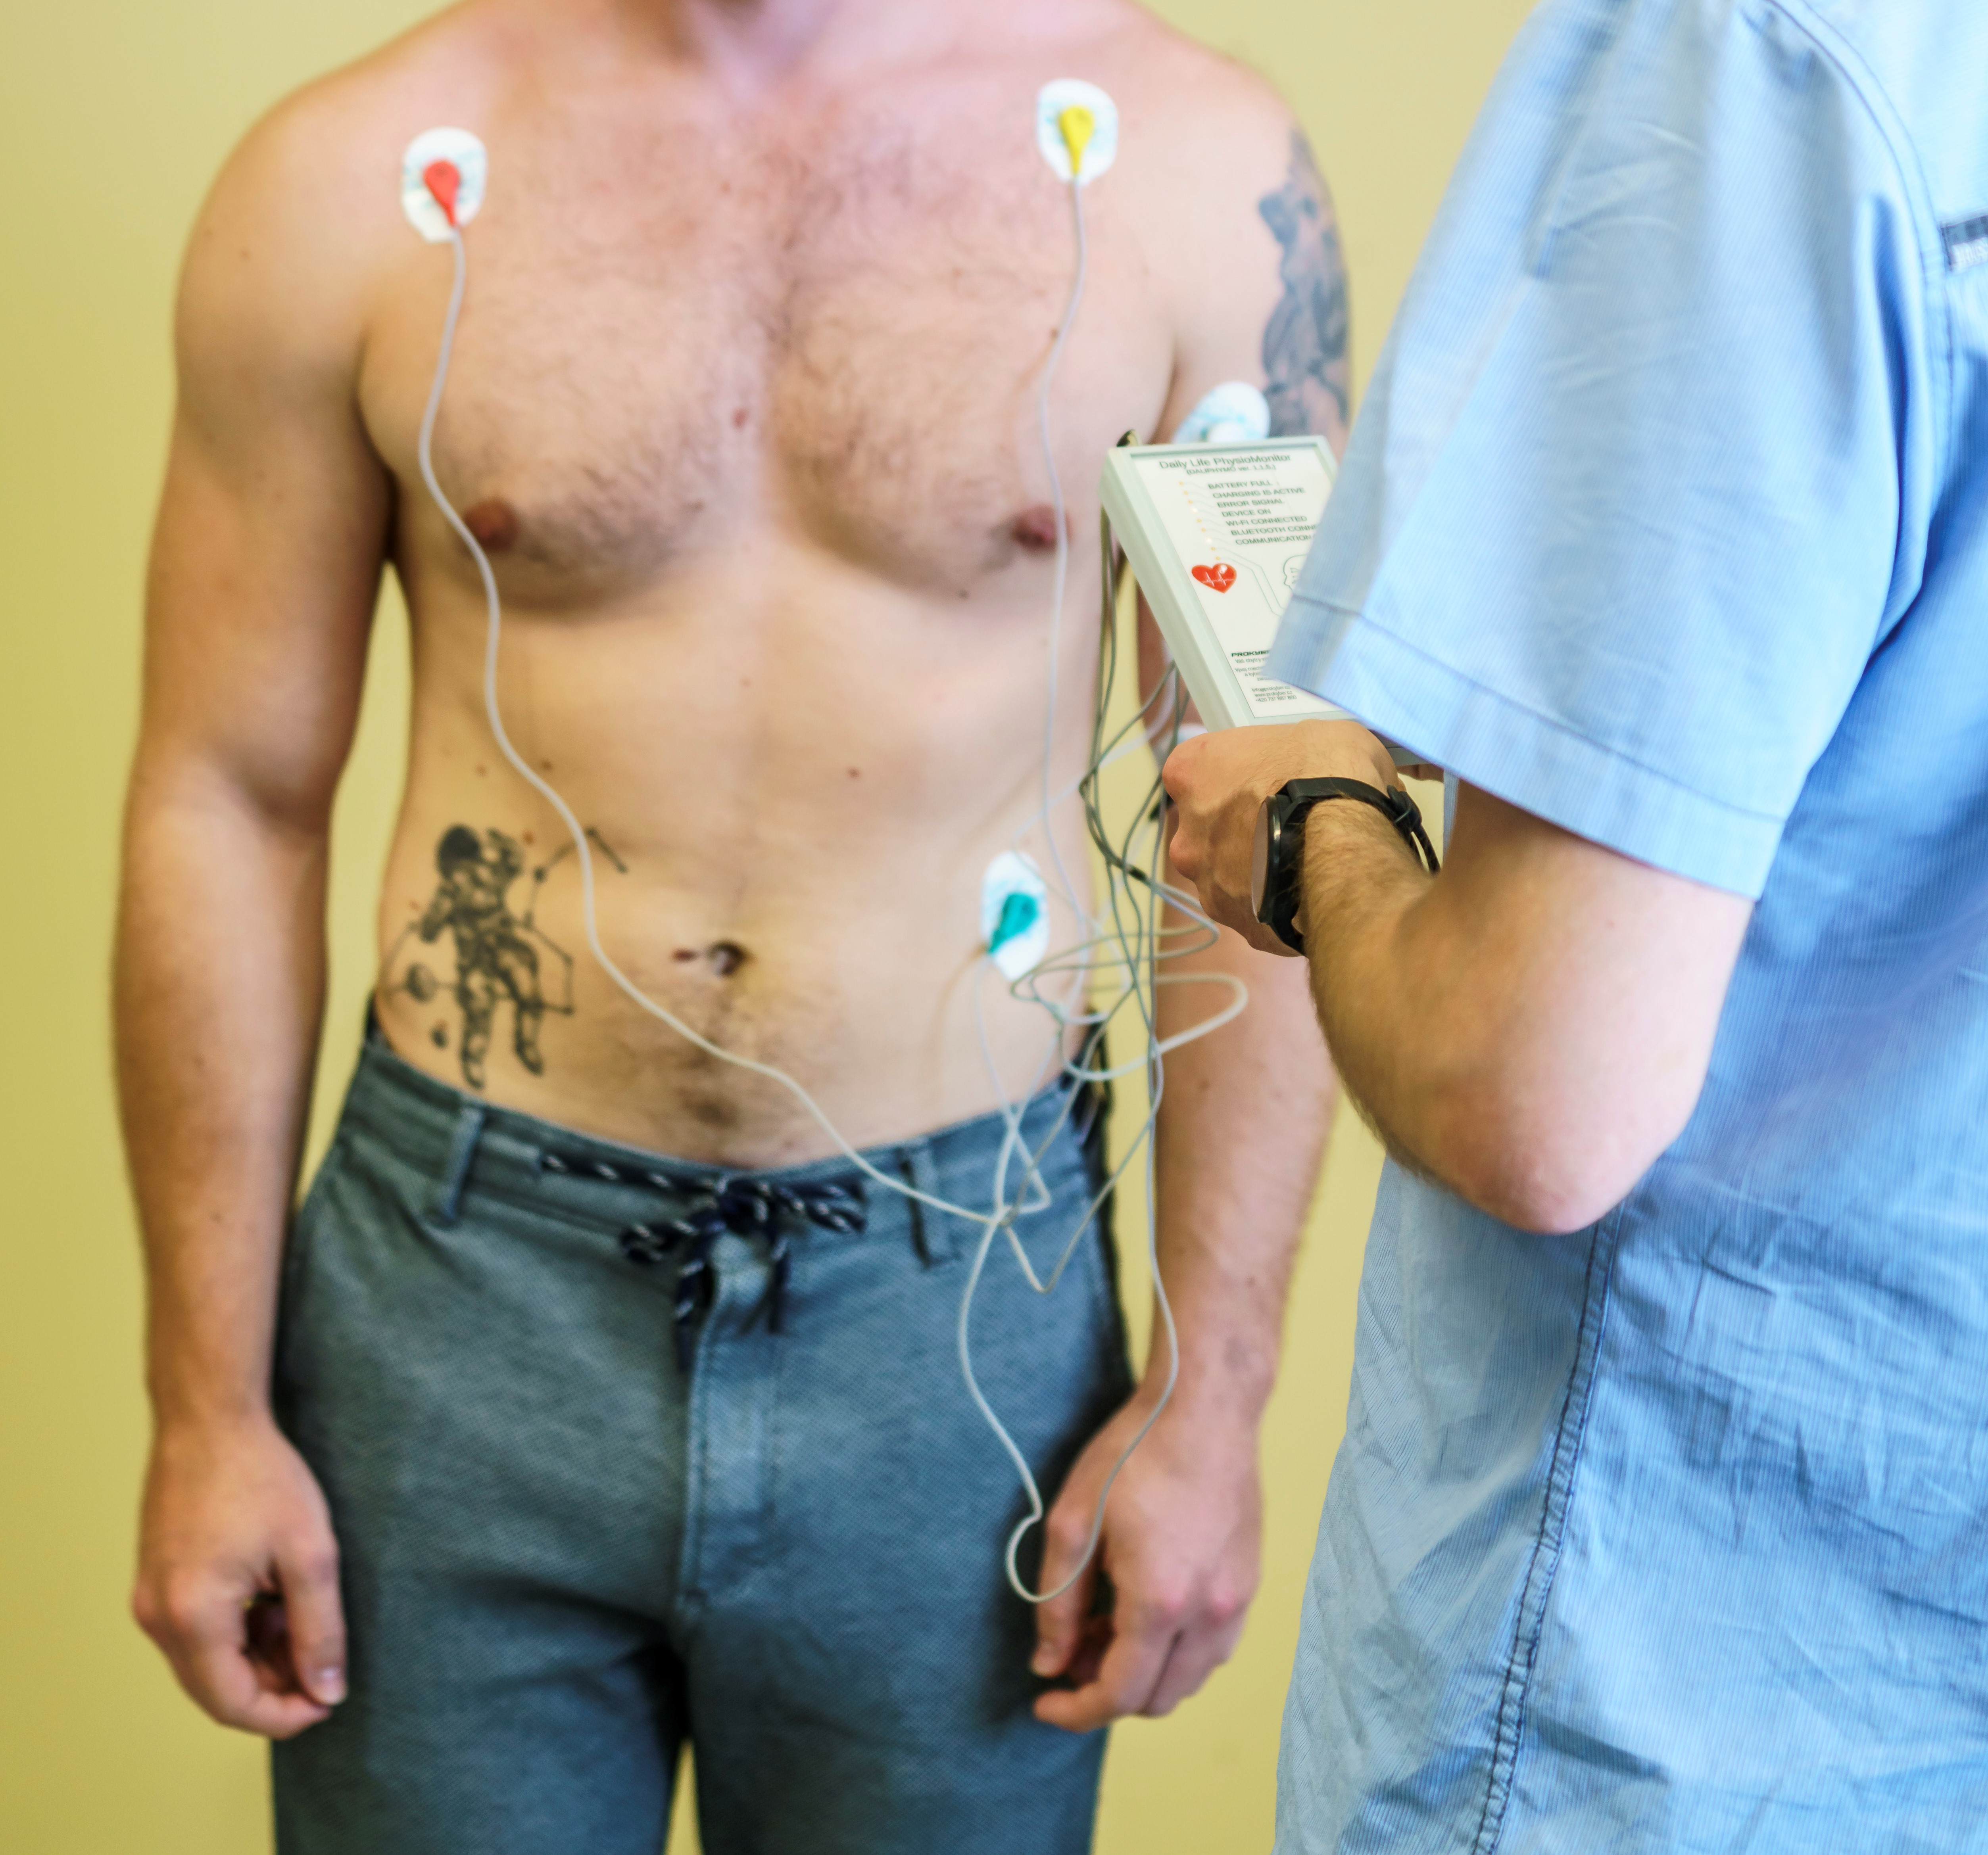
\includegraphics[width=0.7\textwidth]{device/holter2}
        \caption{Měření srdeční aktivity}
        \label{fig:device_usage}
    \end{center}
\end{figure}

\subsubsection{Stroopův test}
\label{section:stroop_test}
Stroopův test (viz Obr.~\ref{fig:stroop}) se řadí mezi psychologické testy osobnosti a byl primárně navržený
pro testování percepční zátěže. Postupem času se možnosti jeho využití
rozšiřovaly~\cite{Svoboda1999}. Dnes je Stroopův test jeden z nejběžnějších
neuropsychologických testů používaný k hodnocení  a stimulaci kognitivní
zátěže~\cite{Scarpina2017}.

\begin{figure}[h]
    \begin{center}
        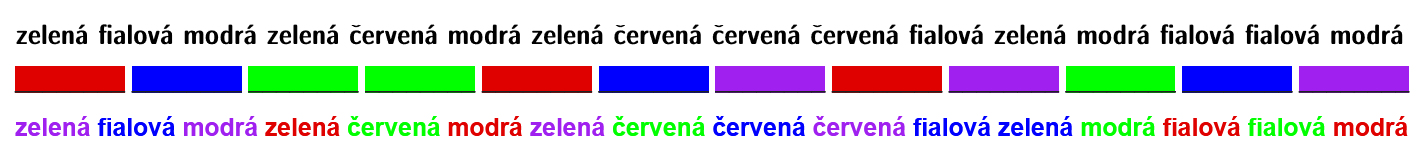
\includegraphics[width=1\textwidth]{figures/stroop}
        \caption{Příklad Stroopova testu~\cite{stroopWiki}}
        \label{fig:stroop}
    \end{center}
\end{figure}

Princip testu spočívá ve třech po sobě následujících krocích. Prvním krokem je
přečtení řady slov, která jsou napsána černou barvou a označují několik barev
(nejčastěji červená, žlutá, zelená a modrá). Dalším krokem je pojmenování každé
jednotlivé barvy v další řadě tvořené barevnými obdélníky. Posledním krokem je
přečtení řady slov, které jsou napsána barevně, ale význam slova této barvě
neodpovídá~\cite{Svoboda1999}.

\subsubsection{Postup měření}
\label{section:measurement_process}
Postup záznamu srdeční aktivity u jednotlivých probandů sestává z
následujících kroků:
\begin{enumerate}
    \item Konfigurace měřícího zařízení podle postupu v sekci~\ref{section:measurement_device}.
    \item Nalepení elektrod na měřeného probanda podle
          Obr.~\ref{fig:device_usage} a připojení příslušných EKG kabelů k elektrodám.
    \item Zapnutí aplikace \textit{BBPM}. Počítač na kterém běží aplikace musí
          být připojený ke stejné síti jako měřící zařízení.
    \item Nastavení aplikace stiskem tlačítka \textbf{Settings} a vyplněním IP
          adresy a portu měřícího zařízení do kolonek \textbf{Host} a \textbf{Port} v
          kartě \textbf{General}.
    \item Ověření validity spojení stiskem tlačítka \textbf{Test connection}.
    \item Připojení aplikace k měřícímu zařízení stiskem tlačítka
          \textbf{Apply} a následně \textbf{Ok}.
    \item Zahájení záznamu srdeční aktivity stiskem tlačítka \textbf{Record} a
          vybrání cílové destinace, kde bude soubor po ukončení záznamu uložen.
    \item Ukončení záznamu po 10 minutách opětovným stiskem tlačítka \textbf{Record}.
\end{enumerate}

\subsection{Studie}
\label{section:study}
Pilotní měření EKG záznamů bylo prováděno na lidských subjektech, tudíž je nutné
mít informovaný souhlas měřených probandů a souhlasné stanovisko etické komise.

\subsubsection{Stanovisko etické komise}
Sběr dat proběhl v rámci výzkumu \textit{Zpátky za volant -- Diagnostický a
rehabilitační nástroj pro osoby po poškození mozku}. Výzkum byl schválen etickou
komisí FBMI ČVUT. Stanovisko etické komise je uvedeno v Příloze
A (viz sekce~\ref{pdf:souhlas}) společně s informovaným souhlasem.

\subsubsection{Kontrolní skupina probandů}
\label{section:probands}
Za účelem otestovaní navrženého řešení (viz kapitola~\ref{section:thesis_aims}) byla naměřena a
zaznamenána srdeční aktivita podle postupu~\ref{section:measurement_process} u
kontrolní skupiny 5 probandů ve věkovém rozmezí 21--23 let bez diagnostikovaných
kardiovaskulárních onemocnění.

\subsubsection{Sledované statistické veličiny}
\label{section:selected_stats_vals}
Výstupem aplikace použité k záznamu srdeční aktivity (viz kapitola~\ref{section:online_processing}) jsou soubory formátu CSV,
kde každý řádek reprezentuje naměřenou výslednou amplitudu elektrické srdeční
aktivity v daný časový okamžik. Díky znalosti vzorkovací frekvence zařízení lze
snadno ke každému záznamu vypočítat časový vektor a pracovat tak v časové
oblasti.

V závislosti na studii byly vybrány následující sledované statistické parametry
Poincarého grafu s vyžitím metody konstrukce elipsy (viz
kapitola~\ref{section:hrv_methods}):
\begin{itemize}[noitemsep]
    \item \textbf{SD1}~\textit{(Standard Deviation)} -- směrodatná odchylka R-R
          intervalů hlavní osy elipsy,
    \item \textbf{SD2}~\textit{(Standard Deviation)} -- směrodatná odchylka R-R
          intervalů vedlejší osy elipsy,
    \item \textbf{SD1/SD2}~\textit{(Standard Deviation ratio)} -- poměr směrodatných odchylek SD1 a SD2.
\end{itemize}

\subsection{Offline zpracování EKG záznamu}
\label{section:offline_processing}
Zpracování EKG záznamů se orientuje podle diagramu na Obr.
\ref{fig:diagram_offline_processing} a je realizováno v prostředí 
\textit{MathWorks MATLAB 2021a}~\cite{MATLAB} s využitím \textit{Signal Processing
Toolboxu}~\cite{matlabSPT}. Jednotlivé části zpracování EKG záznamu jsou rozebrány v
následujících kapitolách.

\begin{figure}[H]
    \centering
    \begin{tikzpicture}[node distance=2.5cm, thick, scale=0.8, every node/.style={scale=0.8}]
        \node (start) [startstop, text width=2cm] {EKG záznam};
        \node (pro1) [process, right of=start, xshift=1.5cm] {Předzpracování};
        \node (pro2) [process, right of=pro1, xshift=1.5cm, text width=3cm] {Detekce komponentů};
        \node (pro3) [process, right of=pro2, xshift=1.5cm, text width=3cm] {Zpracování komponentů};
        \node (stop) [startstop, right of=pro3, xshift=1.5cm, text width=3cm] {Hodnocení záznamu};

        \draw [arrow] (start) -- (pro1);
        \draw [arrow] (pro1) -- (pro2);
        \draw [arrow] (pro2) -- (pro3);
        \draw [arrow] (pro3) -- (stop);
    \end{tikzpicture}
    \caption{Diagram offline zpracování EKG záznamu}
    \label{fig:diagram_offline_processing}
\end{figure}

\subsubsection{Předzpracování signálu}
\label{section:preprocessing}
Nezbytný krok pro jakoukoliv další práci s biosignálem je jeho filtrace. Před
navržením samotného filtru byl proveden rozbor EKG záznamů pomocí FFT. EKG
signál je tak převeden z časové domény do frekvenční funkcí
\texttt{fft(X)}~\cite{matlabFFT}. Z teorie je znám, v jakých frekvencích se
vyskytuje užitečný EKG signál nebo jeho komponenty a v jakých nežádoucí vlivy
(viz kapitola~\ref{section:ecg_processing_theory}). Tyto znalosti byly při
návrhu filtru a posuzování spektra EKG signálu využity. Pro zlepšení představy o
potenciálních artefaktech a užitečných frekvencích byla provedena FFT analýza i
na několika samotných PQRST segmentech. Na Obr.~\ref{fig:spectral_analysis} lze
vidět FFT analýzu EKG signálu a jednoho PQRST segmentu. Z examinace vizuální
stránky spektra plyne několik východisek pro tvorbu filtru. Jsou zde pohybové
artefakty společně s kolísáním nulové izolinie. Ve frekvenčním spektru a v
částech signálu se dále objevuje nepatrný širokopásmový šum, způsobený
myopotenciály. Ve frekvenčním spektru lze vidět tyto nežádoucí složky přibližně
mezi frekvencemi od 0 do 7,5~\si\Hz.

\begin{figure}[h]
    \begin{center}
        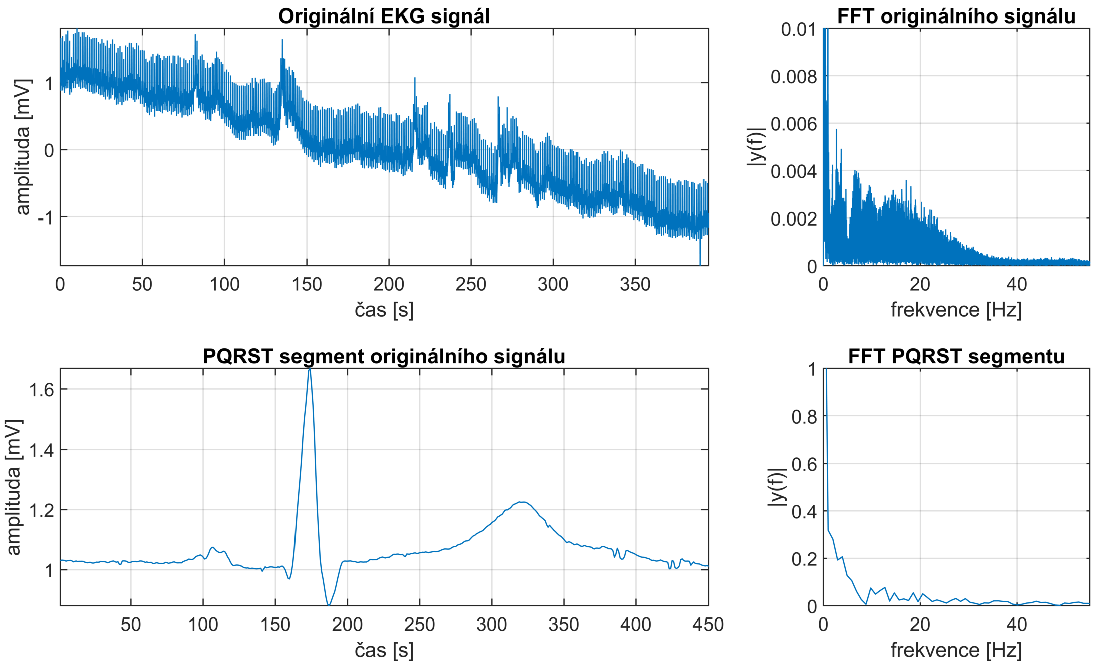
\includegraphics[width=1\textwidth]{figures/spectral_analysis}
        \caption{FFT analýza EKG signálu a QRS komplexu}
        \label{fig:spectral_analysis}
    \end{center}
\end{figure}

Po FFT analýze byl pro potlačení nežádoucích prvků použit pro každý EKG záznam
digitální filtr FIR (viz níže) typu pásmová propust s propustnými frekvencemi v rozmezí
7,5--35~\si\Hz. Filtr byl navržen metodou Kaiserova okna~\cite{Chavan2006},
které je definováno následovně~\cite{Oppenheim1999}:
\begin{equation}
    \label{eq:kaiser1}
    w[n] =
    \begin{cases}
        \frac{I_0[\beta\sqrt{(1-[(n-\alpha)/\alpha]^2)}]}{I_0(\beta)}, & 0 \leq n \leq M \\
        0,                                                           & \text{jinak}.
    \end{cases}
\end{equation}
kde $w$ označuje vypočítané koeficienty, $M$ je počet vzorků, $\alpha=M/2$ a
$I_0(\cdot)$ reprezentuje nultý řád modifikované Besselovy funkce prvního
druhu~\cite{BesselFcn}. Jelikož je potřeba dosáhnout specifického útlumu $A$
(viz kapitola~\ref{section:ecg_processing_theory}), definoval Kaiser parametr
$\beta$ k úpravě zvlnění propustného a závěrného pásma
následovně~\cite{Oppenheim1999}:
\begin{equation}
    \beta =
    \begin{cases}
        0,1102(A-8,7),                      & A > 50            \\
        0,5842(A-21)^{0,4} + 0.07886(A-21), & 21 \leq A \leq 50 \\
        0,                                  & A < 21.
    \end{cases}
\end{equation}

Filtr byl realizován funkcí \texttt{bandpass(x,fpass,fs)}~\cite{matlabBANDPASS}.
Druhou části předzpracování tvoří filtrace zvýrazňující QRS komplexy, konkrétně
R vlny. Použitá metoda pro zvýraznění vychází z vlastností derivace a vyšších
amplitud R vln. Filtrovaný signál je diferencován použitím pěti-bodové diference
prvního řádu dle následujícího vztahu:
\begin{equation}
    \label{eq:differentiation}
    y[n] = \frac{1}{8}(2x[n] + x[n-1] - x[n-3] - 2x[n-4])
\end{equation}
kde $n \geq 5$, $y[n]$ reprezentuje vzorek diferencovaného signálu a $x[n]$
hodnotu původního vzorku. Diference zároveň potlačuje vlivy P a T vln.
Dále je diferencovaný signál umocněn a QRS regiony jsou
následně jednotlivě sloučeny a zvýrazněny využitím zpětné
kumulace~\cite{Wang2017}:
\begin{equation}
    \label{eq:backward_cumulation}
    Bc(n) = \sum_{i=n}^{n+Ww-1} |y(i)|
\end{equation}
s pevnou délkou okna $Ww$ v rozsahu nejdelšího normálního trvání jednoho QRS
komplexu (0,12~\si\s)~\cite{Wang2017}. Ke kumulaci je využívána funkce
\texttt{cumsum(A)}~\cite{matlabCUMSUM}.

\begin{figure}[h!]
    \begin{center}
        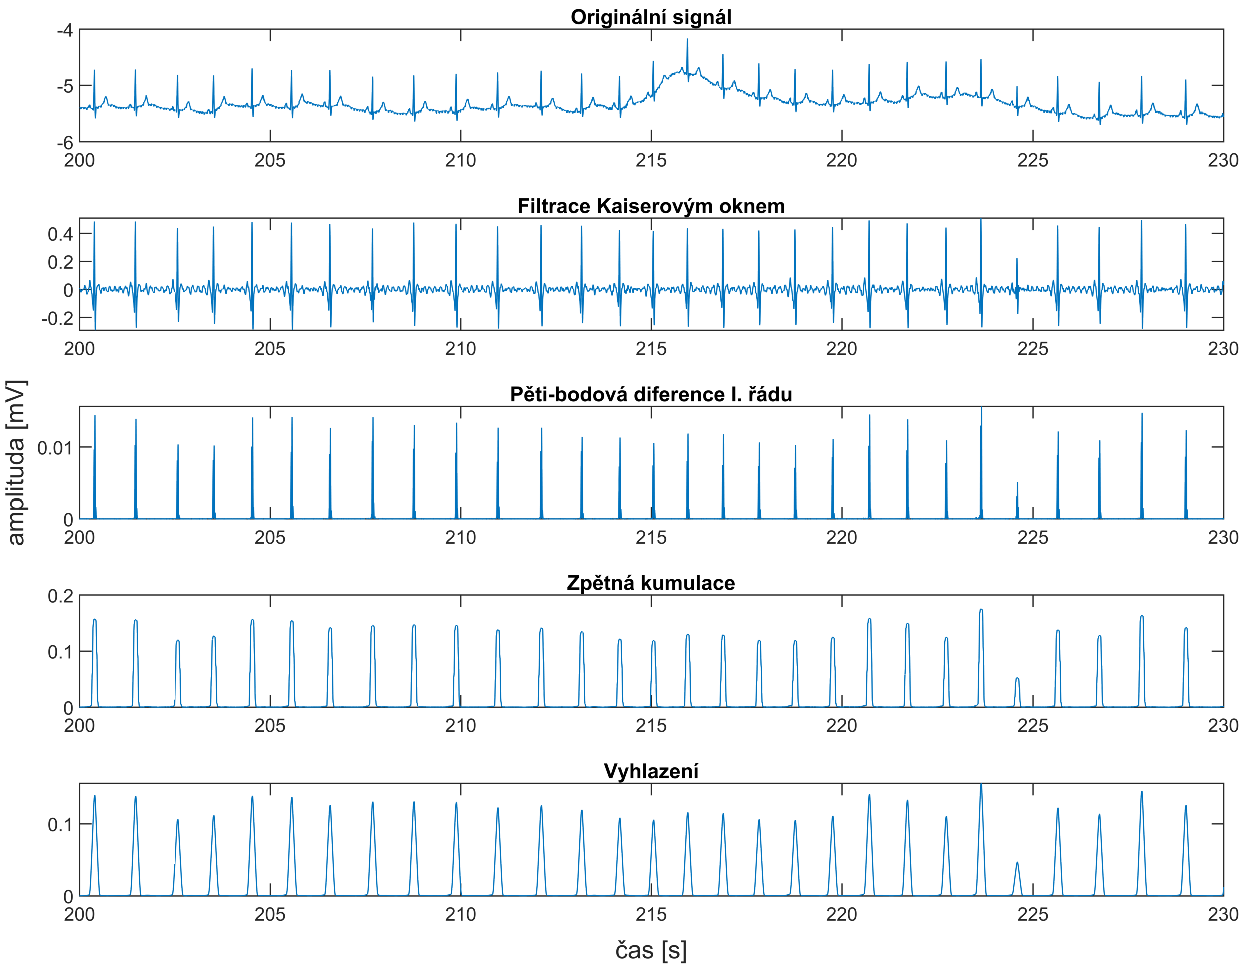
\includegraphics[width=1\textwidth]{figures/preprocessing_steps}
        \caption{Jednotlivé kroky předzpracování EKG signálu}
        \label{fig:preprocessing_steps}
    \end{center}
\end{figure}

Poslední krok předzpracování je vyhlazení vzniklých vrcholů konvolucí použitím
funkce \texttt{conv(u,v)}~\cite{matlabCONV}. Principiálně se jedná o vyhlazení 
plovoucím průměrem s délkou okna 60 vzorků. Délka 60 vzorků je
stejně jako u zpětné kumulace doba trvání QRS komplexu, převedena z času na
počet vzorků pomocí vzorkovací frekvence (500~\si\Hz). Vizuálně lze vidět
jednotlivé kroky předzpracování signálu na Obr.~\ref{fig:preprocessing_steps}.

\subsubsection{Detekce komponentů}
\label{section:components_detection}
Detekce komponentů tvoří nezbytnou část, od které se odvíjí hodnocení EKG
záznamu. Cílem detekce je spolehlivě identifikovat a lokalizovat specifické
komponenty, nejčastěji QRS komplexy, které jsou předmětem analýzy EKG záznamu.
Díky detekovaným komponentům lze signál využitím detekovaných veličin
segmentovat a hodnotit. V první řadě se nejčastěji volí detekce R vln na základě
jejich vysoké amplitudy.

Za účelem detekce R vln byl implementován a modifikován algoritmus
podle~\cite{Nabian2018}, inspirovaný Pan-Tompkinsovou metodou QRS
detekce~\cite{Pan1985} (viz kapitola~\ref{section:components_detection_theory}).
Algoritmus vychází z následujících kroků:
\begin{enumerate}
    \item Iterativní hledání globálních maximálních amplitud s použitím
          plovoucího okna $W$ o délce 400~\si\ms~(0,4~\si\s):
          \begin{gather}
              R_{max} = max(W_i^{L,R}) \nonumber \\
              L = R = \frac{0.4~Fs}{2}, \quad L,R \in \mathbb{Z^+} \nonumber \\
              W_i^{L,R} = \{x_{i-L},...,x_i,...,x_{i+R}\}, \quad \forall i \in \{1+L,...,N-R\}
          \end{gather}
          kde $N$ je počet detekovaných R vln, $Fs$ vzorkovací frekvence, $R_i$
          potenciální R vlna, $x_i$ střed okna a $L$ spolu s $R$ posun od středu
          plovoucího okna. Nalezená maxima nacházející se uprostřed plovoucího
          okna jsou označeny jako potenciální R vlny.
    \item Eliminace všech R vln nižších než než prahová hodnota $Th_{Amp}$, která je v
          každé iteraci rovna 75 \% z průměru amplitud posledních 8 detekovaných
          R vln. Iniciálně je prahová hodnota $Th_{Amp}$ nastavena jako:
          \begin{gather}
              n = 2~Fs, \quad n \in \mathbb{Z^+} \nonumber \\
              Th_{Amp} = \frac{1}{3} max(\{x_1,x_2,x_3,...,x_n\})
          \end{gather}
    \item Výpočet R-R intervalů ($RR_i$) diferencí detekovaných R vln ($R_i$):
          \begin{equation}
              RR_i = R_{i} - R_{i-1}, \quad \forall i \in \{2,...,N\}
          \end{equation}
          Následně je provedena iterativní kontrola vypočítaných R-R intervalů.
          Intervaly delší než prahová hodnota $Th_{RR}$ indikují chybějící R
          vlnu, která je doplněna jako maximální amplituda v rozmezí délky
          plovoucího okna následovně:
          \begin{gather}
              n = \frac{0.4~Fs}{2}, \quad n \in \mathbb{Z^+} \nonumber \\
              R_m = max(\{R_{i+n},...,R_i,...,R_{i+1-n}\}), \quad \forall i \in \{1,...,N\}
          \end{gather}
          kde $R_m$ je doplněná R vlna. Prahová hodnota $Th_{RR}$ je počátečně
          nastavena jako:
          \begin{equation}
              Th_{RR} = 1.66~RR_1
          \end{equation}
\end{enumerate}

Délka plovoucího okna se řídí fyziologickým limitem hodnoty srdečního rytmu v
případech, jako jsou například supraventrikulární tachykardie (SVT) nebo flutter
síní, kde dosahuje srdeční frekvence přibližně 300 úderů za minutu (5 úderů za
sekundu)~\cite{Haberl2012,Goldberger2017}. Dva sousední QRS komplexy se tedy
nemůžou vyskytnout blíže než 200~\si\ms.

\begin{figure}[h]
    \begin{center}
        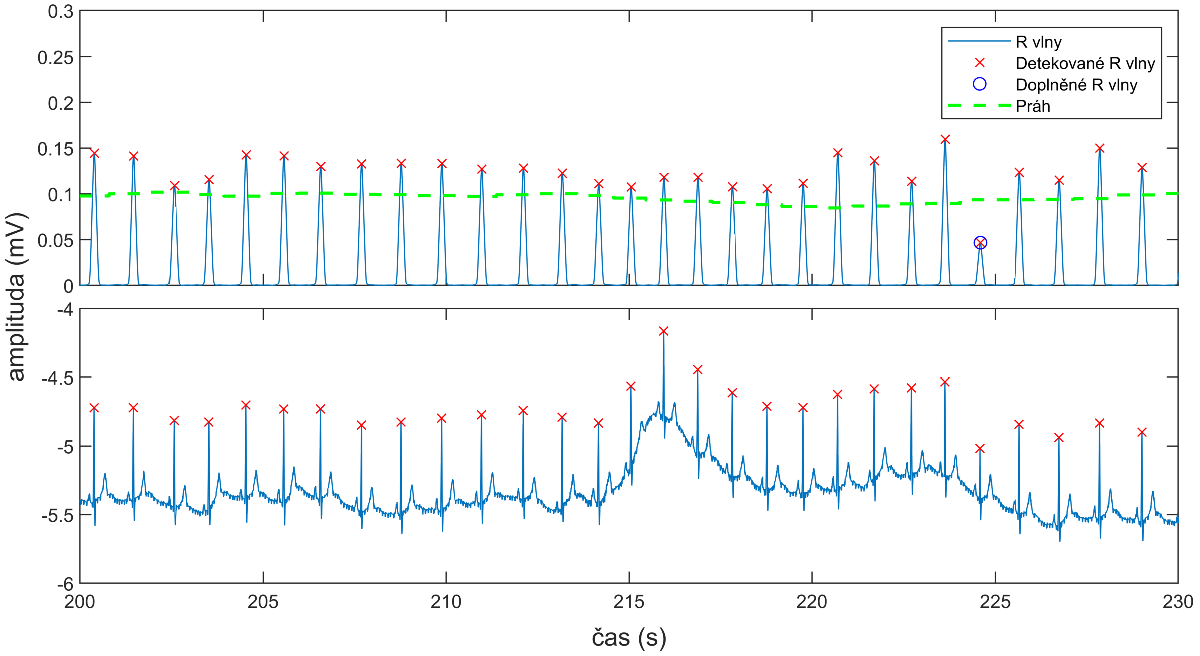
\includegraphics[width=1\textwidth]{figures/detection}
        \caption{Vizualizace detekovaných R vln}
        \label{fig:detection}
    \end{center}
\end{figure}

Na Obr.~\ref{fig:detection} lze vidět zeleně vyznačený
adaptivní práh, který se mění podle 2. kroku výše a doplněnou R vlnu, která
nebyla detekovaná v 1. kroku ale až ve 3. a následně doplněna.

\begin{figure}[H]
    \begin{center}
        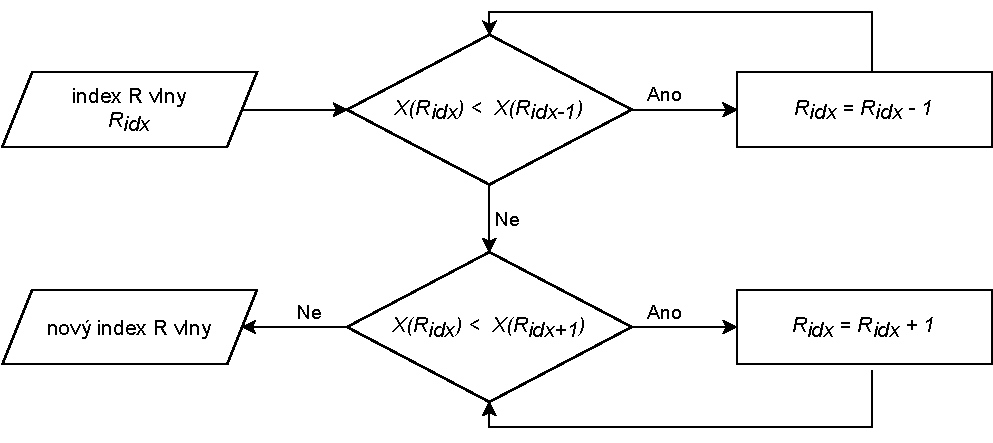
\includegraphics[width=0.87\textwidth]{diagrams/fixpeaks}
        \caption{Algoritmus relokalizace detekovaných R vln}
        \label{fig:fixpeaks}
    \end{center}
\end{figure}

Pro zobrazení detekovaných vln v původním signálu (viz. Obr.~\ref{fig:detection})
byla zavedena metoda relokalizace, která upraví pozice
detekovaných R vln tak, aby souhlasily v původním EKG záznamu. Díky tomu lze
vizuálně ověřit spolehlivost algoritmu nebo evaluovat detekci v oblastech s očekávaným
výskytem artefaktů, které jsou více zatížené nežádoucími vlivy. Postup metody se řídí
diagramem na Obr.~\ref{fig:fixpeaks}, kde $X$ reprezentuje množinu hodnot EKG
signálu.

\subsubsection{Zpracování detekovaných komponentů}
\label{section:components_processing}
V případě analýzy variability srdečního rytmu (viz kapitola~\ref{section:hrv})
je nutné tuto veličinu vypočítat z detekovaných komponentů. Diferencí mezi
sousedícími R vlnami v čase jsou vypočítány R-R intervaly neboli časová
variabilita mezi jednotlivými údery srdce. Stejně jako EKG záznam, tak i R-R
intervaly jsou zatížené artefakty a mohou představovat abnormální hodnoty.
Zdrojem artefaktů jsou nejčastěji falešně nebo nesprávně detekované či chybějící
R vlny a ektopický rytmus, který společně s invalidně detekovanými R vlny
vytváří sekvence dlouhých a krátkých srdečních period. Vizuálně lze artefakty
identifikovat, jako velké náhlé změny či kolísání v grafu jako je tomu na
Obr.~\ref{fig:hrv_artifacts}. Podmínkou HRV analýzy je tedy použití N-N
intervalů (normal-to-normal), které představují korigované R-R intervaly.
Korekcí je myšleno potlačení nežádoucích artefaktů.

\begin{figure}[h]
    \begin{center}
        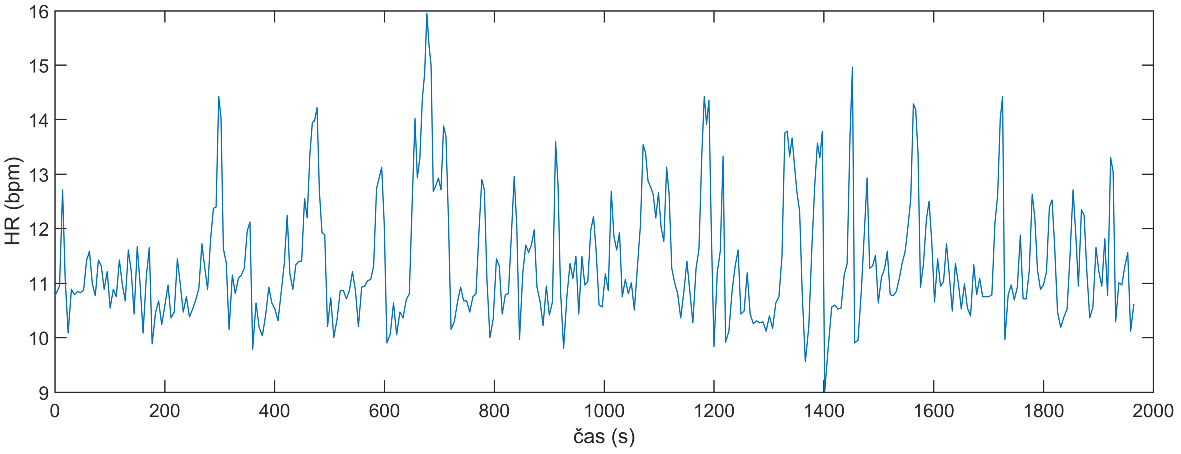
\includegraphics[width=1\textwidth]{figures/hrv_artifacts}
        \caption{HRV signál zatížený artefakty}
        \label{fig:hrv_artifacts}
    \end{center}
\end{figure}

K zajištění spolehlivé HRV analýzy a minimalizaci chyb byla implementována
automatická metoda pro detekci a korekci artefaktů HRV
podle~\cite{Lipponen2019}. Metoda je založená na adaptivním prahování s využitím
dvou pohyblivých prahových hodnot. V prvním kroku je vypočtena časová diference
všech detekovaných R-R intervalů $dRRs$, která slouží k rozlišení ektopických a
nesprávně detekovaných R vln od normálního sinusového rytmu~\cite{Lipponen2019}:
\begin{gather}
    dRRs_1 = 0 \nonumber \\
    dRRs_j = RR_j - RR_{j-1}, \quad \forall j \in \{2,...,N\}
\end{gather}
kde $N$ je počet R-R intervalů. Pro detekci abnormálních intervalů je nastaven
první práh $Th1$, který se adaptuje statistickým odhadem z časově proměnného
rozdělení $dRRs$ hodnot. Práh představuje sérii hodnot, definovaných produktem
faktoru $\alpha$ a mezikvartilového rozpětí $QD$ 91 okolních $dRRs$ intervalů
následovně~\cite{Lipponen2019}:
\begin{equation}
    Th1 = \alpha~QD(|\{dRRs_{j-45},...,dRRs_{j+45}\}|), \quad \forall j \in \{46,...,N-45\}
\end{equation}
kde $\alpha$ je bezrozměrný škálovací faktor, jehož hodnota byla empiricky zvolena
5,2. Časová série $dRRs$ je následně normalizována prahovými
hodnotami~\cite{Lipponen2019}:
\begin{equation}
    dRR_j = \frac{dRRs_j}{Th1_j}, \quad \forall j \in \{1,...,N\}
\end{equation}

Veličiny $dRR$ jsou použité pro detekci ektopických, krátkých, dlouhých nebo
jednotlivě chybějících srdečních period porovnáním $|dRR|>1$. Pro zbylé případy
falešně pozitivní detekce R vln nebo jiných chyb, které nelze detekovat použitím
$dRR$, je definována série $mRRs$ jako rozdíl jednotlivých R-R intervalů a
mediánu 11 okolních hodnot~\cite{Lipponen2019}:
\begin{equation}
    mRRs_j = RR_j - median(\{RR_{j-5},...,RR_{j+5}\}), \quad \forall j \in \{6,...,N-5\}
\end{equation}

Vzhledem k tomu, že při srdeční frekvenci 60 bpm se v rámci falešně pozitivní detekce 
srdečního cyklu hodnota $mRRs$ pohybuje okolo -0,5~\si\s, a při detekci
vynechaného cyklu se blíží k 1~\si\s, nelze použít jednotný práh. Aby bylo
možné použít stejný práh pro všechny případy identifikace artefaktu jako v
předešlé sérii $dRRs$, jsou hodnoty $mRRs$ upravené následující
podmínkou~\cite{Lipponen2019}:
\begin{equation}
    mRRs_j =
    \begin{cases}
        2~mRRs_j, & \forall mRRs_j < 0    \\
        mRRs_j,   & \forall mRRs_j \geq 0
    \end{cases}
    , \quad \forall j \in \{1,...,N\}
\end{equation}

Při stejné srdeční frekvenci (60 bpm) se hodnoty $mRRs$ po úpravě blíží k
0~\si\s~u normálního sinusového rytmu, 1~\si\s~ u vynechaných cyklů a k
--1~\si\s~ u nadbytečně detekovaných srdečních period. Stejně jako pro předchozí
sérii $dRRs$, tak i pro $mRRs$ je zaveden totožně definovaný práh
$Th2$~\cite{Lipponen2019}:
\begin{equation}
    Th2 = \alpha~QD(|\{mRRs_{j-45},...,dRRs_{j+45}\}|), \quad \forall j \in \{46,...,N-45\}
\end{equation}
a hodnoty $mRRs$ jsou následně normalizovány~\cite{Lipponen2019}:
\begin{equation}
    mRR_j = \frac{mRRs_j}{Th2_j}, \quad \forall j \in \{1,...,N\}
\end{equation}

Prahové hodnoty $Th1$ a $Th2$ vycházejí z předpokladu, že časová řada R-R
intervalů pochází z normálního rozdělení, který ve většině případech není
splněn, a proto dochází k chybným identifikacím artefaktů. K zamezení těchto
chyb je metoda doplněna klasifikačním rozhodovacím Algoritmem~\ref{algo:rr_decision}.

\begin{figure}[ht]
    \centering
    \begin{minipage}{.9\linewidth}
        \begin{algorithm}[H]
            \SetKw{Continue}{continue}
            \KwVstup{$S11$, $S12$, $dRR$, $mRR$, $RR$, $Th2$, $rr\_len$ -- Počet R-R intervalů}
            \KwVystup{List detekovaných artefaktů}
            List $\leftarrow$ \{\}\;
            \LinesNumbered
            \For{ $i \in \{1,\ldots,rr\_len-2\}$ }{
                $eq_1 \leftarrow (S11_i > 1) \land (S12_i < (-c_1 \times S11_i - c_1))$\;
                $eq_2 \leftarrow (S11_i < -1) \land (S12_i > (-c_1 \times S11_i + c_2))$\;
                $eq_3 \leftarrow sgn(dRR_i) \times dRR_{i+1} < -1$\;
                $eq_4 \leftarrow sgn(dRR_i) \times dRR_{i+2} < -2$\;
                $eq_5 \leftarrow |RR_i/2 - medRR_i| < Th2_i$\;
                $eq_6 \leftarrow |RR_i + RR_{i+1} - medRR_i| < Th2_i$\;
        
                \If{$|dRR_i| > 1$}{
                        \uIf{ $ eq_1 \land eq_2 $ }{
                            List.append('Ectopic beat'); \Continue;
                        }
                        \uElseIf{$|mRR_i| > 3 \land eq_3 \land eq_4$}{
                            \lIf{$eq_5$}{List.append('Missed beat'); \Continue}
                            \lElseIf{$eq_6$}{List.append('Extra beat'); \Continue}
                            \lElse{List.append('Long/short beat'); \Continue}
                        }
                        \Else{
                            List.append('Normal beat'); \Continue;
                        }
                    }
                }
            \caption{Detekce a klasifikace artefaktů}
            \label{algo:rr_decision}
        \end{algorithm}
    \end{minipage}
\end{figure}

Veličiny $c_1$ a $c_2$ jsou empiricky nastavené konstanty
podle~\cite{Lipponen2019}. Hodnoty $S11$ a $S12$ jsou definované v následujícím
odstavci.

Ektopický rytmus se v sérii hodnot $dRR$ projevuje jako sekvence záporné, kladné
a záporné hodnoty (NPN, N--Negative, P--Positive) nebo kladné, záporné a
kladné (PNP). Pomocí těchto vzorů je rozlišen ektopický rytmus od vynechaných
či nadbytečných srdečních cyklů nebo náhlých změn srdeční frekvence. 
Pro účely vizuálního hodnocení detekce ektopických
srdečních stahů je vytvořen dvoudimenzionální prostor $S1$
následovně~\cite{Lipponen2019}:
\begin{gather}
    S11_j = dRR_j, \quad \forall j \in \{1,...,N\} \nonumber \\
    S12_j =
    \begin{cases}
        max(\{dRR_{j-1}, dRR_{j+1}\}), & dRR_j > 0 \\
        min(\{dRR_{j-1}, dRR_{j+1}\}), & dRR_j < 0
    \end{cases}
    , \quad \forall j \in \{2,...,N-1\}
    \label{eq:subspace1}
\end{gather}
ve kterém se hodnoty $S11$ a $-S12$ zvětšují v rámci determinace NPN vzorem a
zmenšují u PNP případů. Na Obr.~\ref{fig:rr_process} lze vidět vizualizované
prostory $S1$ a $S2$ s vyznačenými hranicemi, vymezující detekované artefakty
podle~\eqref{eq:subspace1} a~\eqref{eq:subspace2}.

\begin{figure}[h]
    \begin{center}
        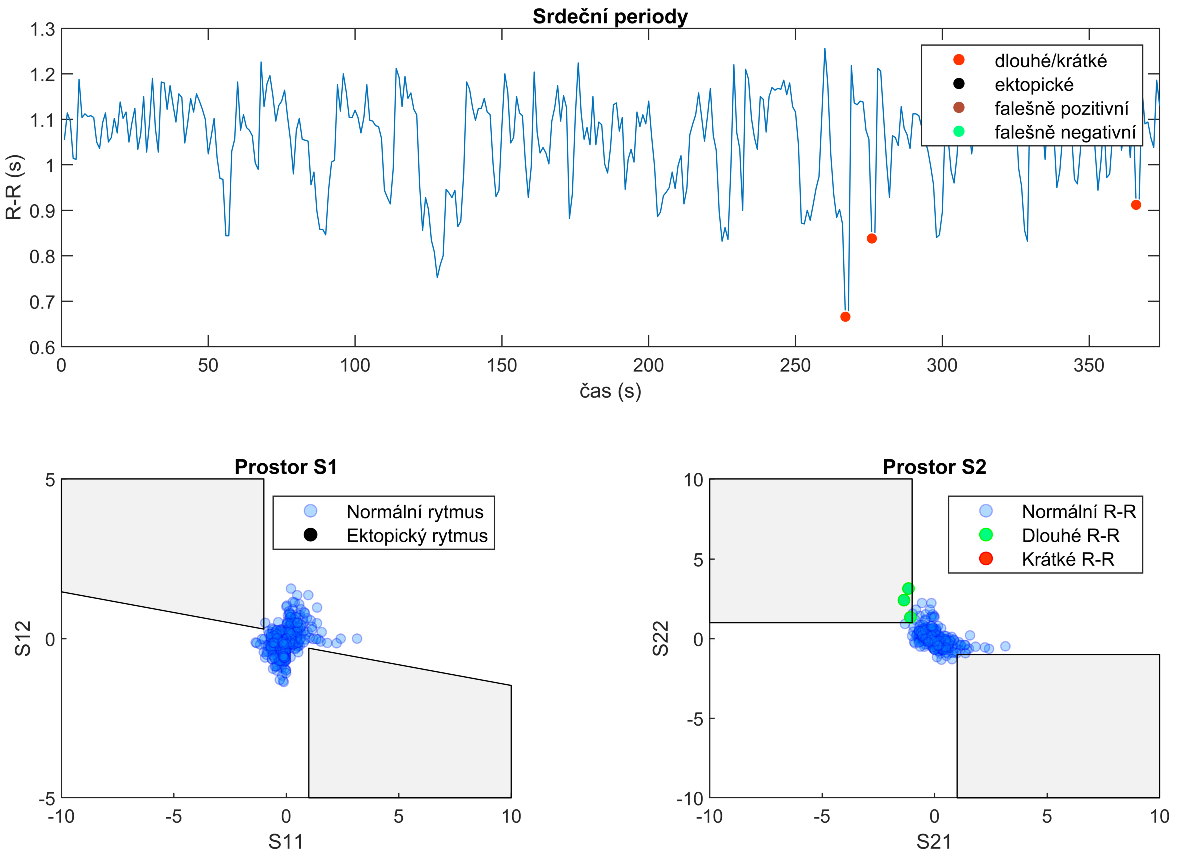
\includegraphics[width=1\textwidth]{figures/rr_process}
        \caption{Vizualizace detekovaných artefaktů}
        \label{fig:rr_process}
    \end{center}
\end{figure}

Dlouhé srdeční cykly včetně případů nedetekovaných R vln se projevují v $dRR$
sérií sekvencí PN, pomalými cykly NP a nadbytečnými periodami jako NNP nebo NPP. K
zobrazení těchto artefaktů a jejich detekčních hranic slouží 2D prostor $S2$
definovaný~\cite{Lipponen2019}:
\begin{gather}
    S21_j = dRR_j, \quad \forall j \in \{1,...,N\} \nonumber \\
    S22_j =
    \begin{cases}
        min(\{dRR_{j-1}, dRR_{j+1}\}), & dRR_j \geq 0 \\
        max(\{dRR_{j-1}, dRR_{j+1}\}), & dRR_j < 0
    \end{cases}
    , \quad \forall j \in \{2,...,N-1\}
    \label{eq:subspace2}
\end{gather}

Posledním krokem je korekce detekovaných artefaktů, která se řídí jejich typem a
přepočet nové série korigovaných R-R intervalů. Úprava je realizována
pro každý typ artefaktu následujícím způsobem~\cite{Lipponen2019}:
\begin{itemize}
    \item \textbf{Falešně pozitivní srdeční periody} -- odstranění
          nadbytečných, nesprávně detekovaných R vln, které jsou začátkem falešné
          periody.
    \item \textbf{Vynechané srdeční periody} -- přidání nových R vln, které
          rovnoměrně rozdělí korespondující R-R interval.
    \item \textbf{Dlouhé a krátké srdeční periody} -- interpolace a přidání
          nových R-R intervalů.
    \item \textbf{Ektopický rytmus} -- nahrazení ektopických period interpolovanými R-R intervaly.
\end{itemize}

\subsubsection{Analýza zpracovaného záznamu}
\label{section:analysis}
Pro analýzu EKG záznamů, konkrétně hodnocení HRV, byla zvolena nelineární
geometrická metoda Poincarého grafu s konstrukcí elipsy (viz
kapitola~\ref{section:hrv_methods}). Jedná se o bodový graf, kde každý bod tvoří
R-R interval vynesený proti následujícímu R-R intervalu. Prvním krokem k
sestrojení grafu je vytvoření časových vektorů následovně~\cite{Mazhar2007}:
\begin{gather}
    \overrightarrow{RR_i} = \{RR_1, RR_2,...,RR_{N}\} \\
    \overrightarrow{RR_{i+1}} = \{RR_2, RR_3,...,RR_{N-1}\}
\end{gather}
kde $N$ je celkový počet R-R intervalů. Dalším krokem je výpočet kvantitativních
parametrů Poincarého grafu SD1 a SD2, které zároveň slouží ke konstrukci
elipsy. Směrodatné odchylky SD1 a SD2 jsou vypočteny jako~\cite{Mazhar2007}:
\begin{equation}
    \text{SD1} = \sqrt{var(x1)}
    \quad \textrm{a} \quad
    \text{SD2} = \sqrt{var(x2)}
\end{equation}
kde $x_1$ a $x_2$ neboli hlavní a vedlejší osy elipsy jsou
rovny~\cite{Mazhar2007}:
\begin{equation}
    x_1 = \frac{\overrightarrow{RR_i}-\overrightarrow{RR_{i+1}}}{\sqrt{2}}
    \quad \textrm{a} \quad
    x_2 = \frac{\overrightarrow{RR_i}-\overrightarrow{RR_{i+1}}}{\sqrt{2}}
\end{equation}

\noindent Elipsa je konstruována využitím jejího vyjádření parametrickými
rovnicemi:
\begin{gather}
    \label{eq:ellipse_parametric}
    x = a \cos \theta \nonumber \\
    y = b \sin \theta
\end{gather}
kde $\theta \in \langle 0, 2\pi \rangle$, $a$ je šířka elipsy a $b$ je její
výška. Za výšku elipsy je dosazena hodnota SD1 a za šířku SD2. Hlavní osa
elipsy leží v případě Poincarého grafu na přímce dané předpisem $y=x$ a elipsa
je tak natočena o 45\degree~($\frac{\pi}{4}$). Vypočítané body z parametrického
vyjádření elipsy~(\ref{eq:ellipse_parametric}) je tedy nutné
rotovat následovně:
\begin{equation}
    \begin{bmatrix}
        X \\
        Y
    \end{bmatrix}
    =
    \overline{RR} +
    \begin{bmatrix}
        \cos \frac{\pi}{4} & -\sin \frac{\pi}{4} \\
        \sin \frac{\pi}{4} & \cos \frac{\pi}{4}
    \end{bmatrix}
    \cdot
    \begin{bmatrix}
        x \\
        y
    \end{bmatrix}
\end{equation}
kde $X$ a $Y$ jsou výsledné body po rotaci o 45\degree. $\overline{RR}$ je
vypočítaný průměr z R-R intervalů a je středem elipsy, do kterého je třeba
elipsu posunout přičtením této hodnoty k oběma souřadnicím. Proměnné $x$ a $y$
jsou předešle vypočítané souřadnice podle~\ref{eq:ellipse_parametric}. 
Realizované Poincarého grafy lze vidět v Příloze C (Obr.~\ref{fig:attachment_poincares_plots}).

\subsection{Online zpracování EKG záznamu}
\label{section:online_processing}
Pro zpracování EKG signálu v reálném čase bylo naprogramované multiplatformní
řešení s grafickým učitelským rozhraním (GUI) pojmenované \textit{BBPM -- Better
bpm}. Zpracování signálu se řídí stejným diagramem jako v
kapitole~\ref{section:offline_processing} na
Obr.~\ref{fig:diagram_offline_processing}. Motivací pro vznik aplikace je
spolupráce s Mgr. et Mgr. Ivetou Fajnerovou, Ph.D. z Národního ústavu duševního
zdraví (NÚDZ). Aplikace je využívána pro hodnocení duševního stavu osob ve
virtuální realitě. Detailněji je program popsán v následujících kapitolách.

\subsubsection{Aplikace pro hodnocení a sběr dat}
Program byl vytvořen pomocí skriptovacího jazyka
Python~\cite{python} s využitím frameworku \textit{PySide2} (viz
sekce~\ref{section:pyside}). Hlavním účelem programu je online zpracování a
vizualizace dat z měřicího zařízení, aby bylo možné sledovat a hodnotit
srdeční aktivitu měřené osoby v reálném čase. Aplikací lze data i
zaznamenávat a vzápětí uložit ve formátu CSV. K zajištěni minimální latence mezi
vizualizací zpracovaných dat a přijatými aktuálními daty, probíhá zpracování
signálu, jeho analýza a záznam paralelně (tzv. multithreading).

\subsubsection{Struktura aplikace}
Aplikaci lze rozdělit na dvě základní rozhraní, frontend a backend. Frontend
poskytuje interaktivní GUI společně s vizualizací zpracovaných dat (viz
kapitoly~\ref{section:gui}~a~\ref{section:visual}). V backend části probíhá v
jednotlivých vláknech (threadech) akvizice a záznam dat včetně výpočetních
procesů spojených se zpracováním EKG signálu (sekce~\ref{section:online_data_process}). 
Strukturu aplikace lze vidět na Obr.~\ref{fig:app_structure}.

\begin{figure}[h]
    \begin{center}
        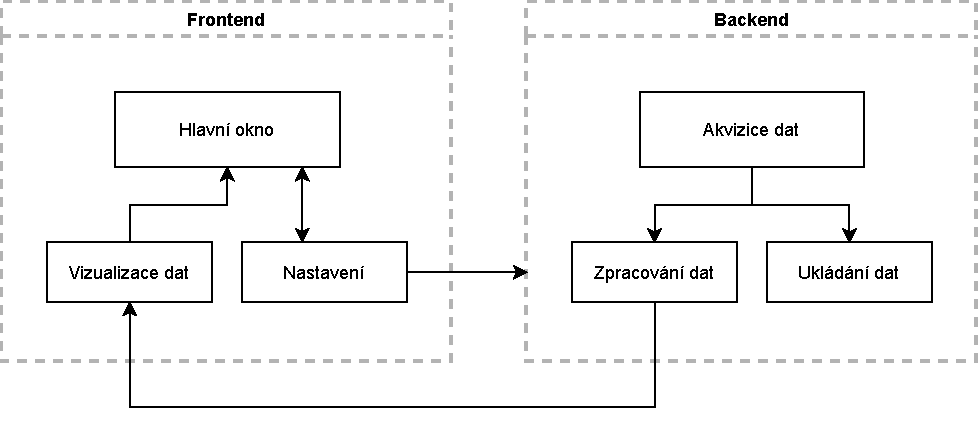
\includegraphics[width=0.9\textwidth]{diagrams/app_structure}
        \caption{Struktura aplikace \textit{BBPM}}
        \label{fig:app_structure}
    \end{center}
\end{figure}

\subsubsection{PySide framework}
\label{section:pyside}
\textit{PySide} představuje vazbu (binding) skriptovacího jazyka Python
na sadu GUI nástrojů populární knihovny \textit{Qt} \cite{Qt}. Díky tomu je
možné využívat aplikační rozhraní (API) knihovny \textit{Qt} v prostředí
Python. \textit{Qt} není pouze knihovna, ale celý nativní
multiplatformní framework pro vytváření softwaru s GUI, implementovaný v programovacím
jazyce \textit{C++}. V aplikaci \textit{BBPM} byla použita knihovna
\textit{PySide2}, která představuje port pro \textit{Qt5}.

\subsubsection{Uživatelské rozhraní}
\label{section:gui}
Grafické uživatelské rozhraní zajišťuje jednoduchou komunikaci mezi aplikací a
uživatelem pomocí interaktivních komponentů. Pro návrh a tvorbu GUI byl použit
nástroj \textit{Qt~Designer}~\cite{QtDesigner}, který je součástí knihovny
\textit{PySide2} a lze vidět na Obr.~\ref{fig:qt_designer}. Nástroj funguje na
principu \textit{WYSIWYG} editorů a umožňuje tak rychlou a intuitivní tvorbu
uživatelského rozhraní. V prostředí nástroje je vidět živý náhled aplikace v
podobě uživatelského okna~(\ref{fig:qt_designer}--\textbf{3}), které je hlavním
komponentem. Do hlavního okna lze z panelu č.~\textbf{1} přesouvat interaktivní
uživatelské prvky. Jednotlivé parametry prvků společně s hlavním oknem (např.
výška a šířka) lze upravovat v panelu č.~\textbf{2}. Vytvořené GUI je možné
následně exportovat v podobě Python kódu nebo formátu UI kompatibilním s knihovnou 
\textit{PySide}.

\begin{figure}[h]
    \begin{center}
        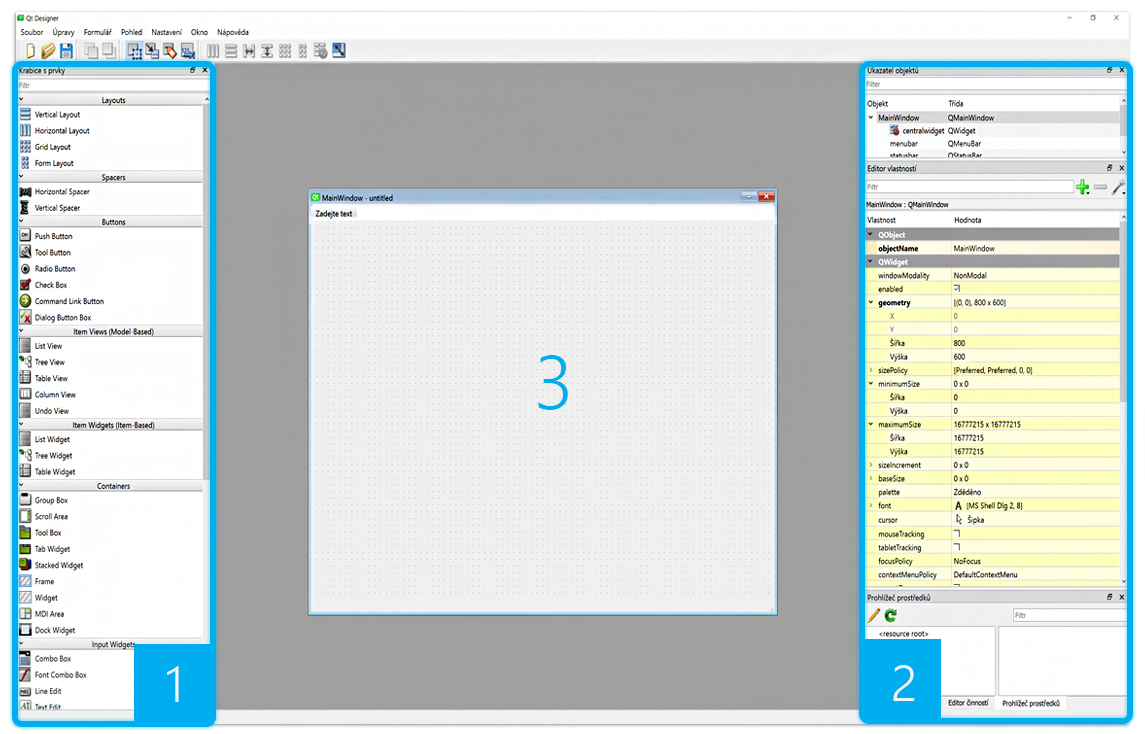
\includegraphics[width=1\textwidth]{bbpm/qt_designer}
        \caption{Prostředí \textit{Qt Designeru}}
        \label{fig:qt_designer}
    \end{center}
\end{figure}

\clearpage

Pro potřeby aplikace byly vytvořena dvě okna -- hlavní okno a okno nastavení.
Hlavní okno (viz Obr.~\ref{fig:app_main_window}) se skládá z postranního
vysouvacího menu~(\ref{fig:app_main_window}-\textbf{1}), které se nachází na
levé straně okna a panelu~(\ref{fig:app_main_window}-\textbf{2}), ve kterém se
zobrazuje karta podle zvolené položky v menu. Vysouvací menu obsahuje čtyři
tlačítka, přičemž první tlačítko, které se nachází v levém horním rohu hlavního
okna, iniciuje vysunutí a zasunutí menu. Jednotlivé funkce ostatních tlačítek
jsou:
\begin{itemize}[noitemsep]
    \item \textbf{Dashboard} -- zobrazení hlavní karty vizualizující výstup,
    \item \textbf{Record} -- zapnutí nahrávání EKG záznamu,
    \item \textbf{Settings} -- vyvolání dialogového okna s nastavením.
\end{itemize}
Postranní menu je modulární, což umožňuje snadné přidání nových položek a k nim
přidružených karet v pravém panelu. Modularita některých funkcí aplikace tak
zajišťuje snadnou rozšiřitelnost v budoucnu.

\begin{figure}[h]
    \begin{center}
        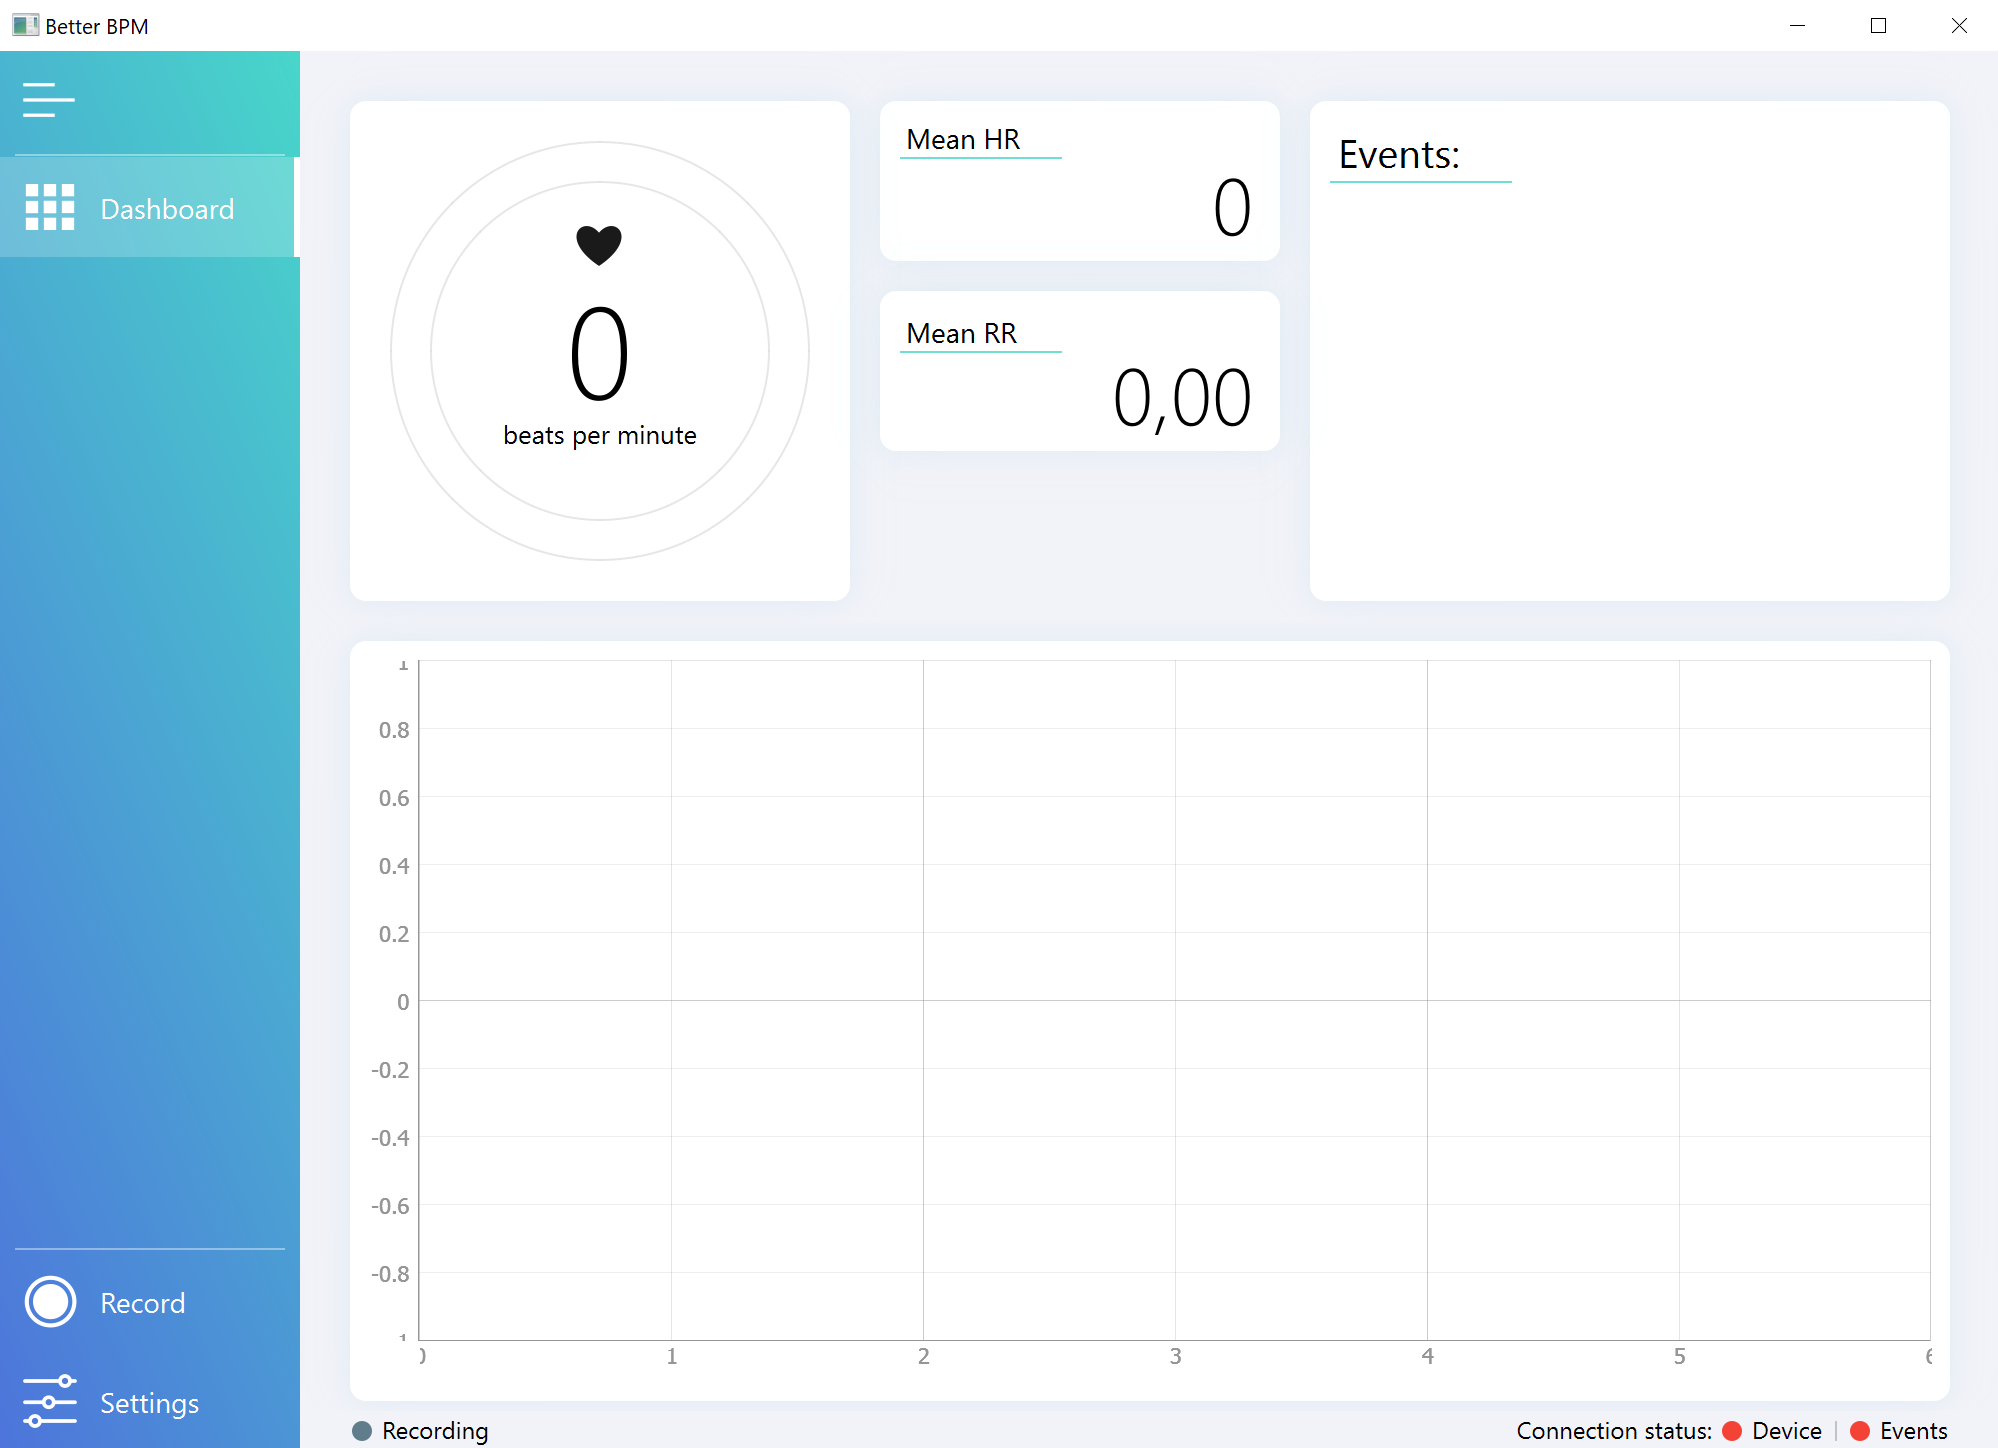
\includegraphics[width=1\textwidth]{bbpm/main_window}
        \caption{Struktura hlavního okna aplikace}
        \label{fig:app_main_window}
    \end{center}
\end{figure}

Karta \textbf{Dashboard} se skládá ze dvou segmentů. Dolní segment karty je
tvořen grafem pro zobrazení EKG křivky~(\ref{fig:app_main_window}-\textbf{4}),
který je detailněji popsán v sekci~\ref{section:visual}. Horní
segment~(\ref{fig:app_main_window}-\textbf{3}) obsahuje čtyři informační
subpanely. První tři zobrazují aktuální srdeční frekvenci, průměrnou srdeční
frekvenci a průměrnou délku R-R intervalů za posledních 6 sekund. První subpanel
zobrazující srdeční frekvenci, zároveň barevně indikuje, zda je její hodnota ve
fyziologickém rozmezí (zelená) nebo je zvýšená, snížená (oranžová) či abnormální
(červená). Rozmezí hodnot bylo zvoleno na základě stanoviska Americké
kardiologické asociace (AHA).

\begin{table}[h]
    \captionsetup{font=small,skip=0.5pt}
    \label{tab:aha_table}
    \catcode`\-=12
    \begin{center}
        \caption{Stanovené hodnoty srdeční frekvence podle AHA}
        \vspace{1ex}
        \setlength{\tabcolsep}{20pt}
        \renewcommand{\arraystretch}{1.3}
        \begin{tabular}{lcc}
            \noalign{\hrule height 2pt}
            \textbf{Srdeční rytmus} &  & \textbf{hodnota (bpm)} \\ \hline
            Bradykardie             &  & < 60                   \\
            Normální                &  & 60--100                \\
            Tachykardie             &  & > 100                  \\ \noalign{\hrule height 2pt}
        \end{tabular}
    \end{center}
\end{table}

Poslední informační subpanel (Events) má uplatnění během měření a hodnocení osob
ve VR v rámci výzkumu \textit{Virtuální město –- herní systém pro kognitivní
    trénink ve virtuálním prostředí}, zmíněného v úvodu
kapitoly~\ref{section:online_processing}. V této práci nemá využití, a proto
není dále blíže popsán.

Okno nastavení obsahuje čtyři záložky (viz Obr. \ref{fig:settings_cards}):
\begin{itemize}
    \item \textbf{General} (Obr.~\ref{fig:settings_general}) -- slouží pro
          nastavení připojovacích údajů k měřícímu zařízení. Tlačítkem \textbf{Test
              connection} lze zkontrolovat připojení.
    \item \textbf{Graph} (Obr.~\ref{fig:settings_graph}) -- slouží k nastavení
          grafu, konkrétně jeho vykreslovacích vlastností. Lze zde nastavit barva a
          tloušťka křivky nebo schovat osy a grid.
    \item \textbf{Recording} (Obr.~\ref{fig:settings_recording}) -- slouží k
          nastavení ID a jména měřené osoby, které se po nahrávání uloží
          společně s naměřenými daty.
    \item \textbf{Info} -- obsahuje informace o verzi aplikace a copyright.
\end{itemize}

\begin{figure}[h]
    \centering
    \begin{subfigure}[t]{0.3\textwidth}
        \centering
        \textcolor{cyan}{\fboxrule=0.5pt\fboxsep=0pt\fbox{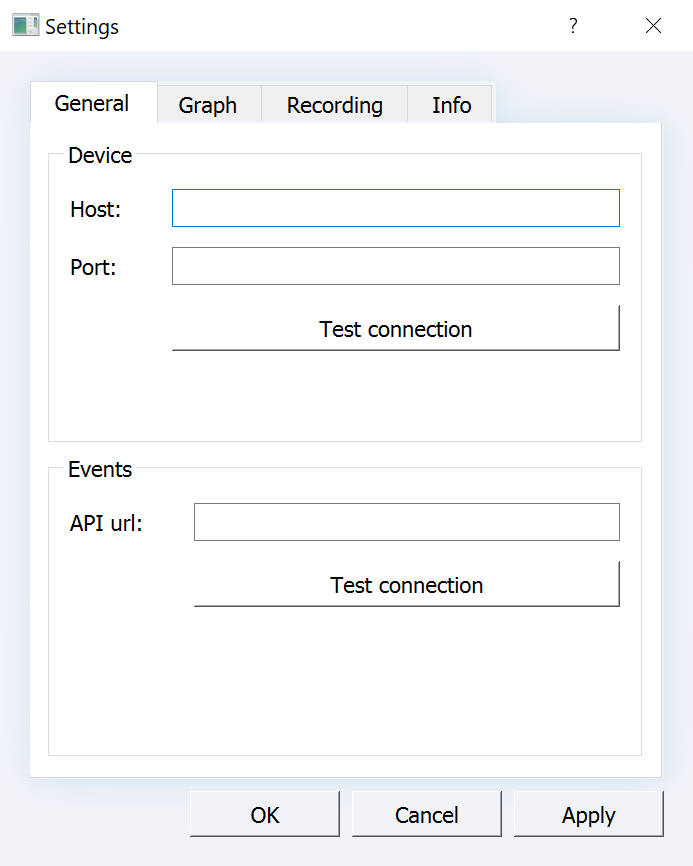
\includegraphics[width=1.05\linewidth]{bbpm/settings_general}}}
        \caption{záložka General}
        \label{fig:settings_general}
    \end{subfigure}
    \hspace{5pt}
    \begin{subfigure}[t]{0.3\textwidth}
        \centering
        \textcolor{cyan}{\fboxrule=0.5pt\fboxsep=0pt\fbox{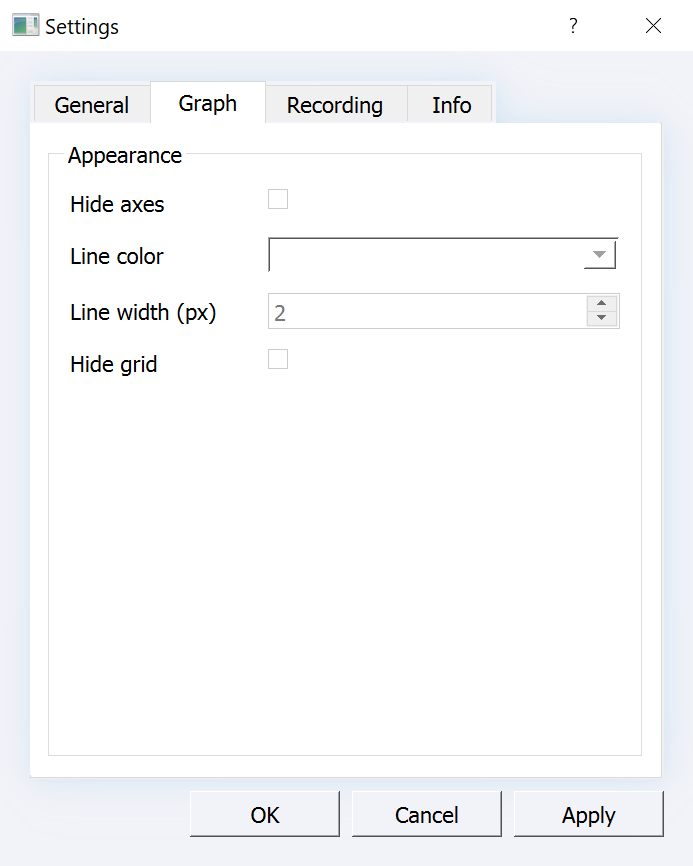
\includegraphics[width=1.05\linewidth]{bbpm/settings_graph}}}
        \caption{záložka Graph}
        \label{fig:settings_graph}
    \end{subfigure}
    \hspace{5pt}
    \begin{subfigure}[t]{0.3\textwidth}
        \centering
        \textcolor{cyan}{\fboxrule=0.5pt\fboxsep=0pt\fbox{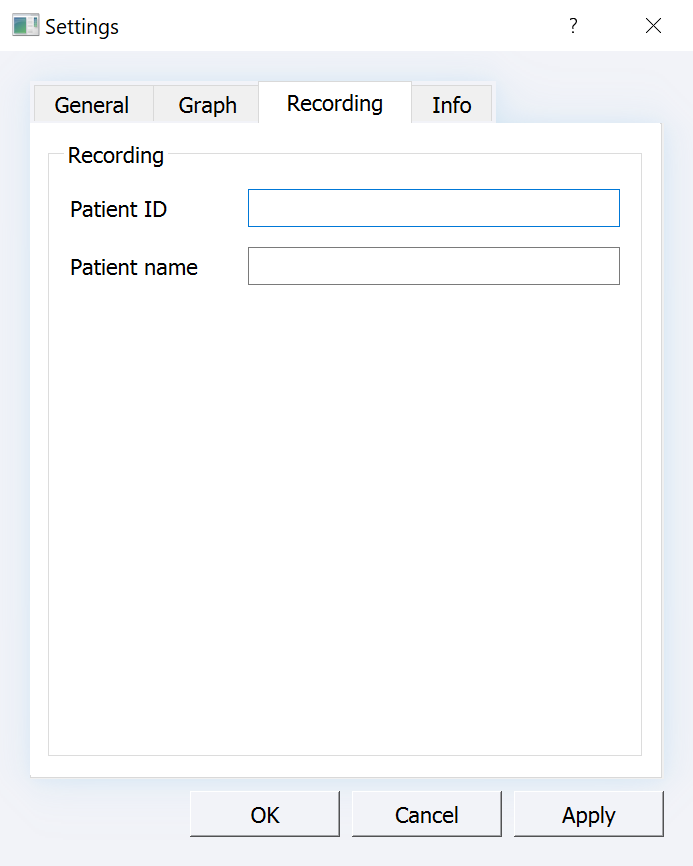
\includegraphics[width=1.05\linewidth]{bbpm/settings_recording}}}
        \caption{záložka Recording}
        \label{fig:settings_recording}
    \end{subfigure}
    \caption{Jednotlivé záložky v okně Nastavení}
    \label{fig:settings_cards}
\end{figure}

\subsubsection{Zpracování dat}
\label{section:online_data_process}
Pro zpracování dat jsou využívané funkce prostředí Python a knihovny
\textit{SciPy}~\cite{SciPy2020}. Před zpracováním EKG signálu jsou přijatá data
nejdříve upravena. Aplikace přijímá z měřícího zařízení v každý jeden okamžik
blok synchronizovaných dat v podobě dvou vektorů o velikosti 2048 hodnot. Jeden
vektor obsahuje hodnoty EKG signálů a druhý časové značky. 

\begin{figure}[h]
    \begin{center}
        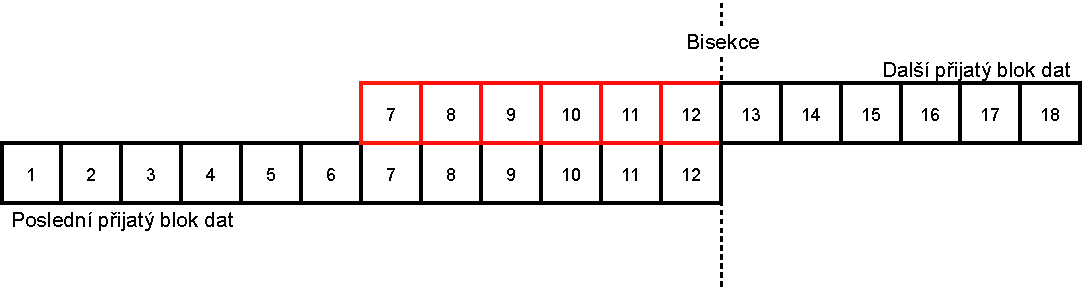
\includegraphics[width=0.9\textwidth]{figures/bisection}
        \caption{Bisekce překrývajících se dat}
        \label{fig:bisection}
    \end{center}
\end{figure}

Jednotlivě přijaté bloky na sebe nenavazují, ale překrývají se (viz Obr.~\ref{fig:bisection}). 
Kontinuita dat je zajištěna použitím algoritmu bisekce, realizovaného funkcí
\texttt{bisect(a,x)}~\cite{bisectRight}, který najde index prvního navazujícího
prvku v závislosti na poslední hodnotě časového vektoru minulého bloku dat.
Překrývající data před tímto indexem jsou odstraněna a podle takto upraveného
časového vektoru je následně upraven i vektor s EKG daty.

Upravené bloky EKG dat jsou předzpracovány filtrem
Savitzky–Golay~(SGF)~\cite{Schafer2011} použitím funkce
\texttt{savgol{\_}filter(x,win{\_}length,order)}~\cite{scipySavgol}. 
SGF je digitální filtr s konečnou impulzní odezvou (FIR), který se
nejčastěji používá k vyhlazení signálu a potlačení jeho vysokofrekvenční složky.
Princip filtru SGF vychází z proložení hodnot v plovoucím okně polynomem
určitého řádu využitím metody nejmenších čtverců. Výsledná hodnota signálu v
daném bodě je vypočtena jako~\cite{wikiSGF}:
\begin{equation}
    y_j = \sum_{i=\frac{1-M}{2}}^{\frac{M-1}{2}} c_j y_{j+i}, \quad \frac{M-1}{2} \leq j \leq N - \frac{M-1}{2}
\end{equation}
kde $c_j$ jsou vypočítané koeficienty polynomiální regrese, $M$ je délka
plovoucího okna a $N$ délka signálu. V aplikaci byla zvolena délka okna 151
vzorků a polynom 3. řádu. Příklad SGF filtrace se zvolenými parametry lze vidět
na Obr.~\ref{fig:sgf_filter}.

Po filtraci jsou data přidána do cyklické fronty~\cite{circlebuffer}, kde
probíhá nepřetržitá detekce komponentů, konkrétně R vln. K detekci je použita
funkce \texttt{find{\_}peaks(x,h,d)}~\cite{scipyFindpeaks}. Funkcí probíhá
hledání lokálních maxim signálu v závislosti na zadané prahové amplitudě a
minimální vzdáleností mezi sousedními R vlnami. Prahová hodnota amplitudy byla
zvolena 0,2~\si\mV~a minimální vzdálenost 0,4~\si\s~(200 vzorků).

\begin{figure}[h]
    \begin{center}
        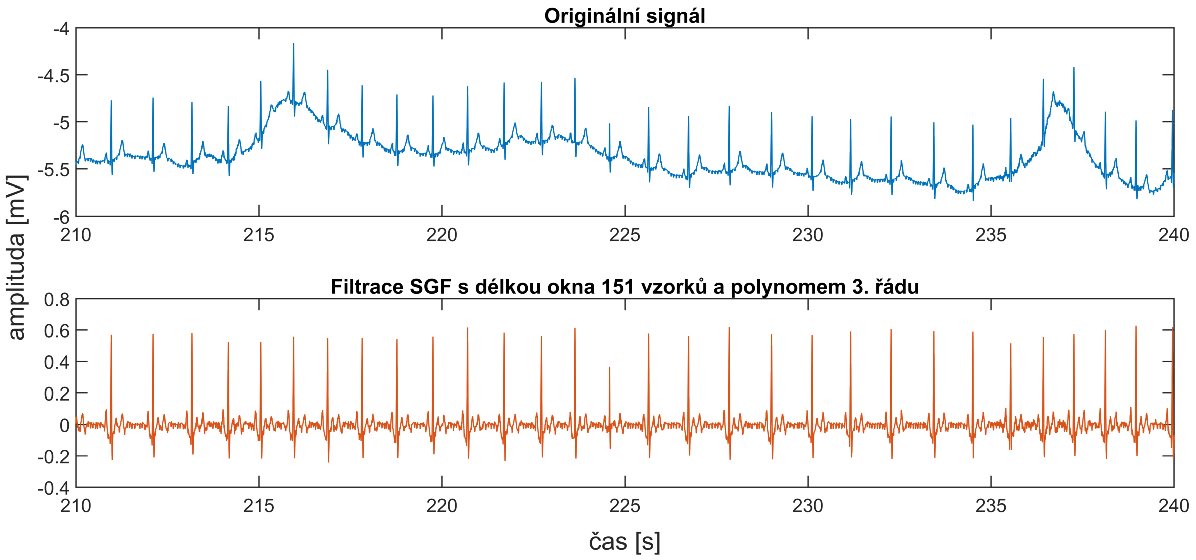
\includegraphics[width=1\textwidth]{figures/sgf_filter}
        \caption{Savitzky–Golay filtrace}
        \label{fig:sgf_filter}
    \end{center}
\end{figure}

Zpracování komponentů (R vln) se odvíjí od zobrazených parametrů na hlavním
panelu aplikace (viz Obr. \ref{fig:app_main_window}). Detekované R vlny slouží k 
výpočtu srdeční frekvence. Diferencí časových hodnot R vln jsou získány R-R intervaly. 
Aktuální srdeční frekvence je poté vypočtena použitím posledního R-R intervalu následovně:
\begin{equation}
    \label{eq:calc_hr}
    HR = \frac{60}{RR}
\end{equation}
kde $HR$ je hodnota srdeční frekvence a $RR$ aktuálně vypočtená srdeční
perioda. Na panelu je z vypočítané hodnoty zobrazena celá část čísla. Dalším
parametrem je průměrná hodnota srdeční frekvence, která se počítá podle
vztahu~\ref{eq:calc_hr} výše. Namísto $RR$ je ale dosazena průměrná hodnota
všech R-R intervalů za posledních 6 sekund, která je posledním počítaným
parametrem podle:
\begin{equation}
    \overline{RR} = \frac{1}{N} \sum_{i=1}^N RR_i
\end{equation}
kde $\overline{RR}$ je vypočítaný průměr R-R intervalů a $N$ je počet R-R
intervalů. Hodnoty se následně zobrazují na panelu v horním segmentu aplikace.

\subsubsection{Vizualizace EKG}
\label{section:visual}
Pro vykreslování dat je použita knihovna \textit{PyQtGraph} \cite{PyQtGraph},
která je plně kompatibilní s frameworkem \textit{PySide2} (viz
sekce~\ref{section:pyside}). Hlavním komponentem této knihovny je graf, kterému
lze funkcí \texttt{setData(x,y)}~\cite{curveItem} předat hodnoty pro osu X a Y.
Po předání jsou hodnoty vykresleny a graf je aktualizován. Předávání hodnot se 
provádí cyklicky, a tak dochází
\begin{figure}[H]
    \begin{center}
        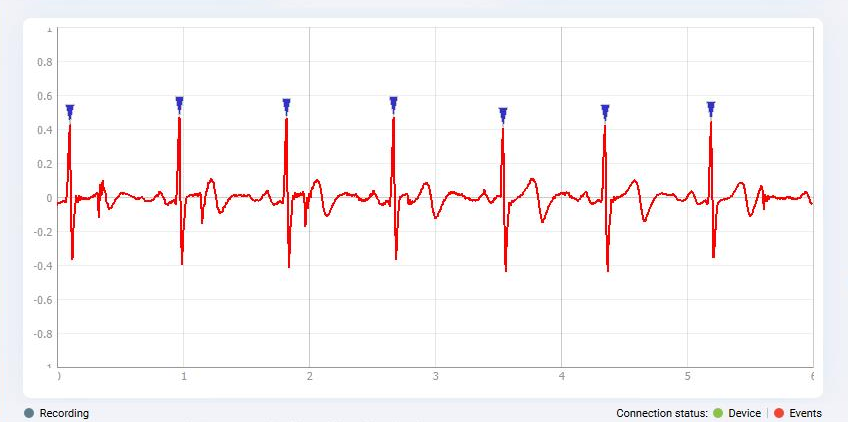
\includegraphics[width=0.75\textwidth]{bbpm/r_detection}
        \caption{Vizualizace EKG křivky s detekcí R vln na hlavním panelu
        aplikace \textit{BBPM}}
        \label{fig:app_ecg_visual}
    \end{center}
\end{figure}
\noindent k neustálému vykreslování nových EKG dat. Zároveň jsou využity hodnoty
detekovaných R vln pro vykreslování markerů v podobě modrých šipek, které tyto
vlny označují. Vizualizace dat na hlavním panelu je vidět na
Obr.~\ref{fig:app_ecg_visual}.

\subsection{Statistické metody}
\label{section:statistical_methods}
Pro zpracování výsledků byly v práci použity statistické testy realizované
funkcemi v prostředí programu \textit{MathWorks MATLAB 2021a}~\cite{MATLAB},
které prověřují platnost nulové hypotézy $H_0$. Nulová hypotéza představuje ve
většině případů tvrzení, že rozdíl mezi testovanými daty není statisticky
významný. Proti $H_0$ se zavadí alternativní hypotéza $H_A$, která nulovou
hypotézu vyvrací. K určení platnosti mezi testovanou nebo alternativní hypotézou
slouží statistické testování, které probíhá následovně:
\begin{itemize}
    \item Definice nulové hypotézy $H_0$ s předpokladem, že platí.
    \item Stanovení náhodného pokusu, kterým bude ověřena hypotéza a náhodné
          veličiny, která bude výsledkem pokusu.
    \item Zvolení hladiny významnosti \textalpha, která vyjadřuje
          pravděpodobnost neoprávněného zamítnutí nulové hypotézy $H_0$, i když platí.
          V bakalářské práci je zvolena hladina významnosti \textalpha~=~0,05 (5~\%).
    \item Zamítnutí nulové hypotézy $H_0$ v případě, že hodnota náhodné veličiny
          spadá do kritického oboru, jelikož nastal jev, který by byl velmi
          nepravděpodobný za platnosti hypotézy $H_0$.
    \item Vyhodnocení statistického testu na základě rozhodnutí o platnosti
          nulové hypotézy $H_0$: přijetí hypotézy $H_0$ (zamítnutí alternativní
          hypotézy $H_A$) nebo zamítnutí hypotézy $H_0$ (přijetí alternativní
          hypotézy $H_A$).
\end{itemize}

Pro testování normality náhodné veličiny byl zvolen Shapirův-Wilkův
test~\cite{wikiSHAPIROWILK} na základě porovnání síly testů pro malé vzorky
podle~\cite{Razali2011}. Nulová hypotéza testu $H_0$ tvrdí, že testovaný vzorek
dat pochází z populace s normálním rozdělením. Test byl proveden použitím funkce
\texttt{swtest(x)}~\cite{matlabSWTEST}.

\subsubsection{Parametrické testy}
\label{section:parametric_tests}
Parametrické varianty testů mohou být uplatněny pouze při splnění podmínky
normality dat. V práci byl použit párový t-test~\cite{Henry2005}, který testuje
rozdíl středních hodnot mezi dvojicí veličin dvourozměrného náhodného výběru.
Test byl realizován funkcí \texttt{ttest(x)}~\cite{matlabTTEST}.
\clearpage

\section{Výsledky}
Kapitola výsledky je rozdělena na čtyři části. První dvě kapitoly prezentují
realizované softwarové řešení pro online a offline hodnocení srdeční aktivity.
Následně sekce~\ref{sections:results_probands} uvádí výsledky analýzy
zpracovaných záznamů a statistického testování normality sledovaných veličin
(viz kapitola~\ref{section:selected_stats_vals}).
Sekce~\ref{sections:results_analysis} popisuje výsledky statistického ověření
metody Poincarého grafu v rámci hodnocení HRV u zpracovaných EKG záznamů.

\subsection{Softwarové řešení pro offline hodnocení EKG}
\label{sections:results_online}
Výstup jednotlivých fází zpracování EKG záznamů (viz kapitola
\ref{section:offline_processing}) byl sjednocen do jednoho hlavního okna pomocí
integrovaného \textit{App Designeru} \cite{matlabAPPDESIGNER} v programovém
prostředí MATLAB. Výsledkem je spustitelná interaktivní aplikace. Po
spuštění aplikace lze v menu pomocí tlačítka \textbf{Load signal} nahrát EKG
signál ve formátu CSV nebo MAT. Po výběru EKG signálu je uživatel tázán aby
zadal vzorkovací frekvenci signálu. EKG signál je následně adaptivně zpracován.
\begin{figure}[h]
	\begin{center}
		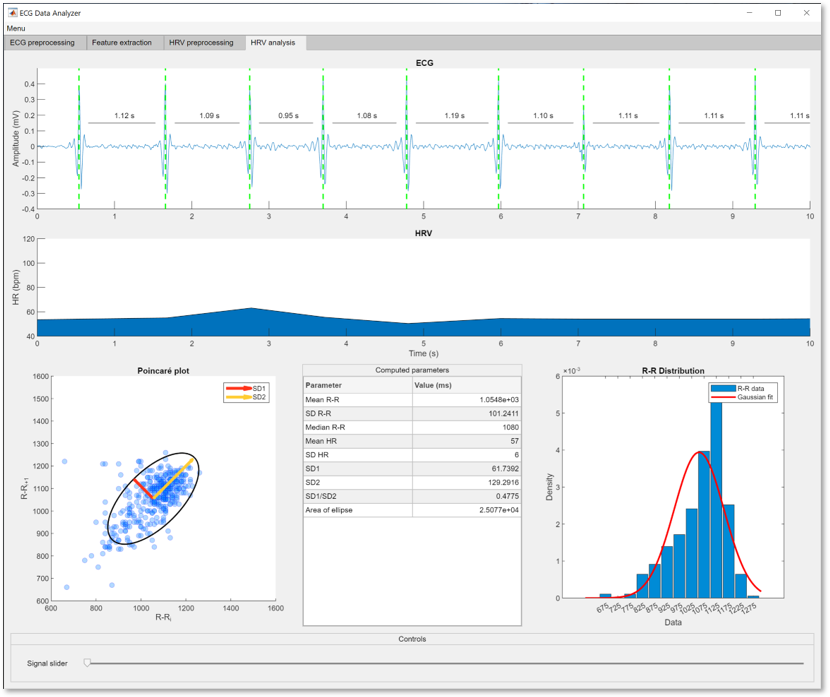
\includegraphics[width=1\textwidth]{matlab_EDA/tab4}
		\caption{Hlavní okno aplikace -- karta HRV analysis}
		\label{fig:results_matlab_tab4}
	\end{center}
\end{figure}
Na Obr.~\ref{fig:results_matlab_tab4} lze vidět otevřenou kartu \textbf{HRV
analysis}, která vizualizuje výstup HRV analýzy vycházející ze všech předešlých
fází zpracování. Všechny karty aplikace jsou uvedené v Příloze B. Jednotlivé
karty jsou mezi sebou propojené. Pokud například uživatel v jedné kartě posune
signál na určitý čas, tak se tato změna aplikuje na signály ostatních karet.

\subsection{Softwarové řešení pro online hodnocení EKG}
\label{sections:result_offline}
Pro účely online analýzy EKG a sběr dat byla naprogramovaná aplikace jménem
\textit{BBPM} v prostředí Python. Prostředí \textit{Python} bylo
zvoleno na základě jeho open-source licence, která jej umožňuje zdarma používat
a volně nebo i komerčně distribuovat vyvinutá řešení. Aplikaci lze vidět na
Obr.~\ref{fig:results_bbpm}. Realizované řešení bylo použito pro pilotní měření
a záznam surových EKG signálů u kontrolní skupiny probandů (viz
kapitola~\ref{section:probands}). Aplikace je detailněji popsaná v
kapitole~\ref{section:online_processing}.

\begin{figure}[H]
	\begin{center}
		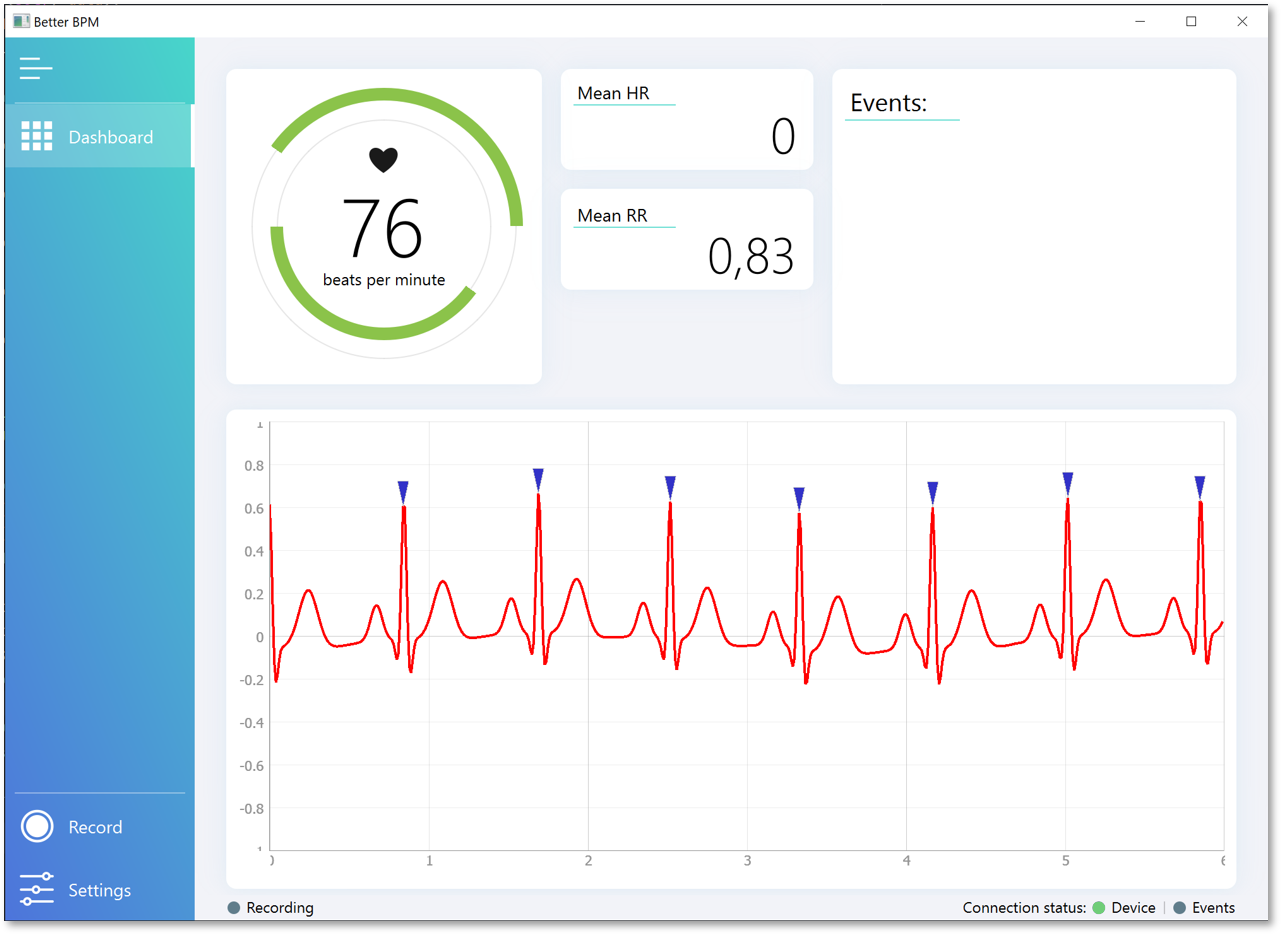
\includegraphics[width=1\textwidth]{bbpm/bbpm_app}
		\caption{Aplikace \textit{BBPM}}
		\label{fig:results_bbpm}
	\end{center}
\end{figure}

\clearpage

\subsection{Kontrolní skupina}
\label{sections:results_probands}
V rámci kontrolní skupiny (viz sekce~\ref{section:probands}) bylo dle postupu v
kapitole~\ref{section:measurement_methodology} naměřeno 5 EKG záznamů aplikací
\textit{BBPM} (\ref{section:online_processing}). Záznamy byly následně
zpracované realizovaným SW řešením popsaným v
sekci~\ref{section:offline_processing}. V následujících podkapitolách jsou
prezentovány výsledky jednotlivých fází zpracování realizovaného offline řešení
pro hodnocení EKG.

\subsubsection{Detekované R vlny}
Následující tabulka \ref{tab:detected_artifacts} uvádí výstup fáze zpracování
detekovaných komponentů společně s vypočítanými parametry: průměrná hodnota
korigovaných (normálních, N-N) R-R intervalů (mNN), průměrná hodnota srdeční
frekvence (mHR), směrodatná odchylka R-R intervalů (SDNN) a směrodatná odchylka
srdeční frekvence (SDHR). Hodnoty parametrů vychází z R vln, který byly
korigovány algoritmem popsaným v sekci~\ref{section:measurement_process}. Z
korigovaných veličin vychází následná HRV analýza. Detekované artefakty uvádí
Tab.~\ref{tab:detected_artifacts}.

\begin{table}[h]
	\captionsetup{skip=0.5pt}
	\catcode`\-=12
	\begin{center}
		\caption{\label{tab:corrected_components} Korigované R vlny s vypočítanými parametry časové série R-R intervalů z klidové částí měření (N) a při Stroopově testu (S)}
		\vspace{1ex}
		\setlength{\tabcolsep}{13pt}
		\renewcommand{\arraystretch}{1.3}
		\begin{tabular}{llccccc}
			\noalign{\hrule height 2pt}
			                    &   &                      & \multicolumn{4}{c}{\textbf{Vypočítané parametry (ms)}}                                                 \\	\cline{4-7}
			                    &   &                      & \textbf{mNN}                                           & \textbf{mHR}  & \textbf{SDNN} & \textbf{SDHR} \\
			                    &   & \textbf{Počet R vln} & \small{(ms)}                                           & \small{(bpm)} & \small{(ms)}  & \small{(bpm)} \\	\noalign{\hrule height 2pt}
			\textbf{1. proband} & N & 369                  & 957                                                    & 64            & 139           & 10            \\
			                    & S & 428                  & 1043                                                   & 58            & 114           & 7             \\	\noalign{\hrule}
			\textbf{2. proband} & N & 374                  & 1055                                                   & 57            & 101           & 6             \\
			                    & S & 270                  & 982                                                    & 62            & 81            & 5             \\	\noalign{\hrule}
			\textbf{3. proband} & N & 535                  & 635                                                    & 95            & 49            & 7             \\
			                    & S & 542                  & 586                                                    & 103           & 52            & 9             \\	\noalign{\hrule}
			\textbf{4. proband} & N & 539                  & 649                                                    & 93            & 56            & 8             \\
			                    & S & 607                  & 536                                                    & 113           & 47            & 10            \\	\noalign{\hrule}
			\textbf{5. proband} & N & 447                  & 920                                                    & 67            & 142           & 10            \\
			                    & S & 321                  & 897                                                    & 68            & 91            & 7             \\ 	\noalign{\hrule height 2pt}
		\end{tabular}
	\end{center}
\end{table}

\subsubsection{Detekované artefakty R-R intervalů}
Včetně korigovaných R vln jsou výstupními parametry fáze zpracování detekovaných
komponentů také detekované artefakty. Počty detekovaných
artefaktů za celý 10 minutový EKG záznam jsou pro každého probanda vyneseny v
Tab.~\ref{tab:detected_artifacts}. Detekce artefaktů, společně se způsoby
korekce jejich jednotlivých typů, je popsaná v
sekci~\ref{section:components_processing}.

\begin{table}[h]
	\captionsetup{skip=0.5pt}
	\catcode`\-=12
	\begin{center}
		\caption{\label{tab:detected_artifacts} Detekované artefakty v časové sérii R-R intervalů}
		\vspace{1ex}
		\setlength{\tabcolsep}{11pt}
		\renewcommand{\arraystretch}{1.3}
		\begin{tabular}{llcccc}
			\noalign{\hrule height 2pt}
			                    &  & \multicolumn{4}{c}{\textbf{Srdeční periody (počet artefaktů)}}                                                                     \\	\cline{3-6}
			                    &  & \textbf{Ektopické}                                             & \textbf{Dlouhé/krátké} & \textbf{Nadbytečné} & \textbf{Vynechané} \\	\hline
			\textbf{1. proband} &  & 2                                                              & 6                      & 1                   & 5                  \\
			\textbf{2. proband} &  & 3                                                              & 0                      & 0                   & 3                  \\
			\textbf{3. proband} &  & 7                                                              & 0                      & 0                   & 12                 \\
			\textbf{4. proband} &  & 0                                                              & 0                      & 0                   & 0                  \\
			\textbf{5. proband} &  & 0                                                              & 3                      & 0                   & 3                  \\	\noalign{\hrule height 2pt}
		\end{tabular}
	\end{center}
\end{table}

\subsection{Analýza EKG záznamu pomocí Poicarého grafu}
\label{sections:results_analysis}
Pro kvantitativní hodnocení srdeční aktivity pomocí Poincarého grafu počítá
realizovaná MATLAB aplikace v rámci HRV analýzy pro každý zpracovaný
EKG záznam veličiny SD1, SD2 a jejich poměr SD1/SD2. Vypočítané sledované
veličiny ze dvou úseků EKG záznamů každého probanda uvádí
Tab.~\ref{tab:poincare_parameters}. Během prvního úseku byli probandi měřeni
v klidu (situace N) a v druhém úseku podstoupili Stroopův test (situace S), který
stimuluje kognitivní zátěž. Metodika měření je detailněji popsaná v
sekci~\ref{section:measurement_methodology}.

\begin{table}[h]
	\captionsetup{skip=0.5pt}
	\catcode`\-=12
	\begin{center}
		\caption{\label{tab:poincare_parameters} Vypočítané sledované veličiny z klidové částí měření (N) a při Stroopově testu (S)}
		\vspace{1ex}
		\setlength{\tabcolsep}{21pt}
		\renewcommand{\arraystretch}{1.3}
		\begin{tabular}{lllccc}
			\noalign{\hrule height 2pt}
			                    &  &   & \multicolumn{3}{c}{\textbf{Poincaré parametry (ms)}}                                   \\	\cline{4-6}
			                    &  &   & \textbf{SD1}                                         & \textbf{SD2} & \textbf{SD1/SD2} \\	\noalign{\hrule height 2pt}
			\textbf{1. proband} &  & N & 96.43                                                & 170.56       & 0.57             \\
			                    &  & S & 79.34                                                & 139.18       & 0.57             \\ 	\noalign{\hrule}
			\textbf{2. proband} &  & N & 61.38                                                & 129.22       & 0.48             \\
			                    &  & S & 43.22                                                & 105.58       & 0.41             \\	\noalign{\hrule}
			\textbf{3. proband} &  & N & 28.60                                                & 62.81        & 0.46             \\
			                    &  & S & 20.94                                                & 70.35        & 0.30             \\	\noalign{\hrule}
			\textbf{4. proband} &  & N & 18.93                                                & 77.53        & 0.24             \\
			                    &  & S & 13.69                                                & 65.63        & 0.21             \\	\noalign{\hrule}
			\textbf{5. proband} &  & N & 80.70                                                & 174.04       & 0.46             \\
			                    &  & S & 57.21                                                & 115.77       & 0.49             \\	\noalign{\hrule height 2pt}
		\end{tabular}
	\end{center}
\end{table}

Za účelem srovnání shod sledovaných veličin mezi situacemi N a S byla nejdříve
vyšetřena normalita dat pomocí Shapirova-Wilkova testu normality (viz
sekce~\ref{section:statistical_methods}). Výsledky jsou vyneseny v
Tab.~\ref{tab:normality_tests}.

\begin{table}[h]
	\captionsetup{skip=0.5pt}
	\catcode`\-=12
	\begin{center}
		\caption{\label{tab:normality_tests} Výsledky testů normálního rozdělení sledovaných veličin ($n=5$)}
		\vspace{1ex}
		\setlength{\tabcolsep}{20pt}
		\renewcommand{\arraystretch}{1.3}
		\begin{tabular}{lccc}
			\noalign{\hrule height 2pt}
			                 &  & \multicolumn{2}{c}{\textbf{Nulová hypotéza vyvrácena}}                              \\ 	\cline{3-4}
			                 &  & \textbf{V klidu (N)}                                   & \textbf{Stroopův test (S)} \\	\noalign{\hrule}
			\textbf{SD1}     &  & Ne                                                     & Ne                         \\
			\textbf{SD2}     &  & Ne                                                     & Ne                         \\
			\textbf{SD1/SD2} &  & Ne                                                     & Ne                         \\	\noalign{\hrule height 2pt}
		\end{tabular}
	\end{center}
\end{table}

V případě všech sledovaných veličin -- SD1, SD2 a SD1/SD2 -- u obou situací N
a S nebyla použitím Shapirova-Wilkova testu na hladině významnosti 5 \%
vyvrácena nulová hypotéza. Lze tedy předpokládat, že vzorky pocházejí ze
základních souborů s normálním rozdělením.

Vzhledem k splnění předpokladů normality bylo u jednotlivých sledovaných veličin
realizované srovnání mezi případy N a S parametrickým párovým t-testem (viz
sekce~\ref{section:parametric_tests}). Výsledky jsou zaneseny v
Tab.~\ref{tab:t_tests}.

\begin{table}[h]
	\captionsetup{skip=0.5pt}
	\catcode`\-=12
	\begin{center}
		\caption{\label{tab:t_tests} Výsledky parametrických testů shody sledovaných veličin mezi klidovou částí měření (N) a při Stroopově testu (S) ($n=5$)}
		\vspace{1ex}
		\setlength{\tabcolsep}{23pt}
		\renewcommand{\arraystretch}{1.3}
		\begin{tabular}{lccc}
			\noalign{\hrule height 2pt}
			                 &  & \textbf{p hodnota} & \textbf{Nulová hypotéza vyvrácena} \\	\noalign{\hrule}
			\textbf{SD1}     &  & 0.0132             & Ano                                \\
			\textbf{SD2}     &  & 0.0967             & Ne                                 \\
			\textbf{SD1/SD2} &  & 0.2363             & Ne                                 \\	\noalign{\hrule height 2pt}
		\end{tabular}
	\end{center}
\end{table}

Pro lepší přehled a srovnání sledovaných veličin byla vytvořena grafická
reprezentace vypočítaných parametrů SD1, SD2 a SD1/SD2. Veličiny vyznačené na
Obr.~\ref{fig:results_sd_vals} odpovídají výsledkům vyneseným v
Tab.~\ref{tab:poincare_parameters}. Dále jsou pro každého probanda v Příloze C
uvedeny jednotlivé výsledné Poincarého grafy, na kterých lze porovnat rozdíly
rozložení R-R intervalů mezi situacemi N a S.

\begin{figure}[H]
	\centering
	\begin{subfigure}[b]{0.3\textwidth}
		\centering
		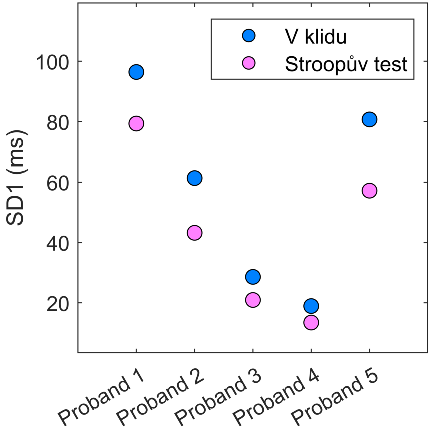
\includegraphics[width=1.1\linewidth]{figures/results_sd1}
		\caption{hodnoty SD1}
		\label{fig:results_sd1}
	\end{subfigure}
	\hfill
	\begin{subfigure}[b]{0.3\textwidth}
		\centering
		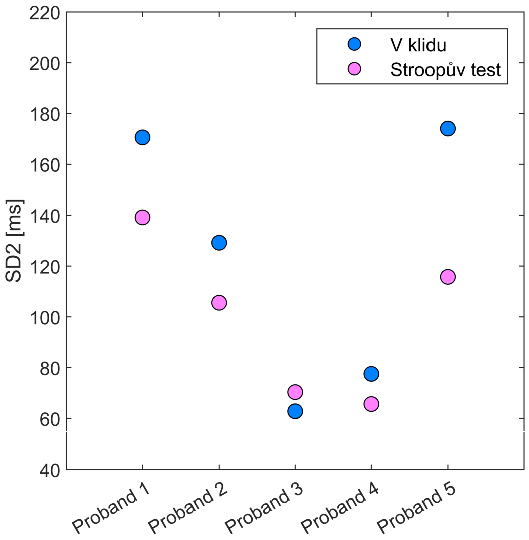
\includegraphics[width=1.1\linewidth]{figures/results_sd2}
		\caption{hodnoty SD2}
		\label{fig:results_sd2}
	\end{subfigure}
	\hfill
	\begin{subfigure}[b]{0.3\textwidth}
		\centering
		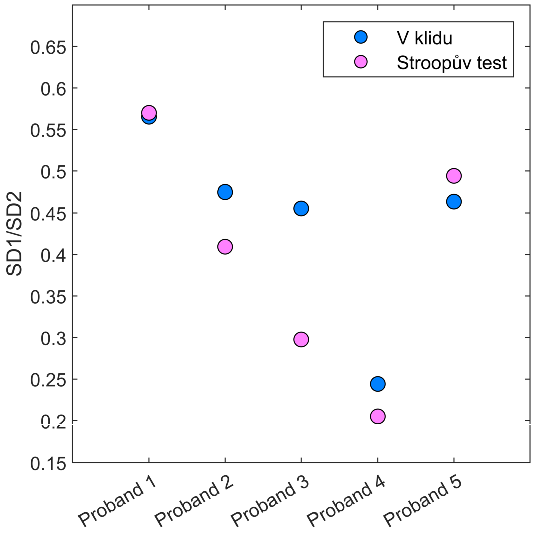
\includegraphics[width=1.1\linewidth]{figures/results_sd1sd2}
		\caption{hodnoty SD1/SD2}
		\label{fig:results_sd1sd2}
	\end{subfigure}
	\caption{Grafické porovnání sledovaných veličin v situacích N a S}
	\label{fig:results_sd_vals}
\end{figure}
\clearpage

\section{Diskuse}
V této části shrňte získané výsledky (hlavní zjištění práce) a následně tyto výsledky interpretujte s ohledem na cíle práce. 
Lze též získané výsledky a výstupy konfrontovat s výsledky a výstupy jiných autorů, výrobky jiných společností apod. 
Nezbytné je správné uvádění zdrojů (citace prací, které jsou zde porovnávány a diskutovány). 
Diskutují se rovněž limitace práce. 
Nakonec lze nastínit další směřování práce do budoucna, opatrně spekulovat o klinickém významu práce apod.

Struktura a obsah této části je detailně probírána a procvičována v příslušných seminářích na oboru BMT. 

\clearpage

\section{Závěr}
V rámci bakalářské práce bylo navrženo a realizováno softwarové MATLAB
řešení pro offline zpracování a hodnocení srdeční aktivity. Řešení je založeno
na postupu, který se skládá z částí předzpracování, detekce komponentů,
zpracování komponentů a analýzy. Za účelem detekce komponentů byl zaveden a
modifikován QRS detektor využívající adaptivní prahování. Pro zpracování
komponentů byl implementován komplexní algoritmus, který detekuje a koriguje
artefakty v rámci detekovaných komponentů. Hodnocení srdeční aktivity probíhá v
časové oblasti a je založeno na nelineární geometrické metodě Poincarého grafu.
Předmětem analýzy je variabilita srdeční frekvence. Realizované řešení
jednotlivé částí vizualizuje společně s Poincarého grafem a automaticky počítá
jeho kvantitativní parametry využitím metody proložení elipsou. 

Dále byla navržena a naprogramována multiplatformní aplikace v prostředí Python
pro online hodnocení srdeční aktivity. Pro aplikaci bylo vytvořeno grafické
uživatelské rozhraní, které uživateli umožňuje jednoduché interaktivní ovládání
aplikace. Software je založený na zpracování EKG signálu v reálném čase, který
je přijímán z měřicího zařízení přes bezdrátovou lokální síť. Zároveň v reálném
čase probíhá detekce komponentů, ze kterých jsou vypočteny vybrané parametry 
z časové oblasti. Aplikace poskytuje živou vizualizaci určených parametrů a 
zpracovaného EKG signálu na jejím hlavním panelu. Byla přidána i funkcionalita 
pro sběr surových nebo zpracovaných dat.

Pomocí navržené Python GUI aplikace bylo provedeno pilotní měření EKG na 
kontrolní skupině 5 probandů. Použitím realizovaného MATLAB řešení
byly záznamy zpracovány a analyzovány. Jednalo se o krátkodobé 10 minutové záznamy.
Na základě výsledků analýzy byly určeny sledované veličiny a vyšetřeny rozdíly mezi
úseky EKG záznamů, kdy byl proband v klidu nebo vystaven kognitivní zátěží. 

Bylo realizováno ověření navržených řešení statistickým zpracováním vyšetřených
rozdílů sledovaných veličin. V rámci celé kontrolní skupiny byl pozorován
statisticky významný rozdíl sledované veličiny SD1, do které se promítají
krátkodobé změny HRV podmíněné vlivem parasympatiku. Dominance parasympatiku je
spojena s aktivitou prefrontálního kortexu, který lze stimulovat kognitivní
zátěží. Ke stimulaci kognitivní zátěže byl u kontrolní skupiny využit Stroopův
test. Zjištěné výsledky potvrzují spolehlivost analýzy realizovaného řešení a
možnost využití Poicarého grafu jako kvantitativního ukazatele změn v ANS. 

\subsection{Budoucí práce}
V rámci projektu \textit{Virtuální město} (viz sekce~\ref{section:online_processing}) 
bude aplikce \textit{BBPM} nadále vyvíjena. Pro zvýšeni uživatelské přívětivosti budou 
některé funkce aplikace automatizovány. Například automatické vyhledávání a připojení 
měřícího zařízení na lokální bezdrátové sítí. Aplikace bude rovněž rozšířena o lokální
měření přes sériové porty, aby bylo možné používat k měření i zařízení, která nejsou
bezdrátové. Předpokladem je i rozšíření sledovaných veličin během hodnocení v reálném 
čase a potenciální implementace offline analýzy záznamů v časové nebo frekvenční oblasti. 

Vzhledem k čerstvému vydání nové verze frameworku \textit{PySide6}, který je využíván v rámci 
aplikace \textit{BBPM} (viz sekce~\ref{section:pyside}), dojde pravděpodobně k přechodu na 
tuto novější verzi. Na základě tohoto přechodu bude pozměněn i životní cyklus aplikace.

Dále se plánuje rozšíření dosavadně používaných formátů pro ukládání dat (CSV) o formát 
DICOM (Digital Imaging and Communications in Medicine). Formát DICOM je standardní 
formát pro zobrazování, distribuci a uchovávání medicínských dat. 


\clearpage

%-------------Literatura-------------------
\clearpage
\renewcommand{\refname}{Seznam použité literatury} 	% Přejmenování Reference
\addcontentsline{toc}{section}{Seznam použité literatury}     % Přidání této kapitoly do obsahu
\printbibliography
\clearpage

%-------------Přílohy----------------------
\section*{Příloha A: Ukázka softwarového MATLAB řešení}
\label{app:pozadavky}
\addcontentsline{toc}{section}{Příloha A: Ukázka softwarového MATLAB řešení}

\begin{figure}[H]
    \begin{center}
        \textcolor{cyan}{\fboxrule=0.3pt\fboxsep=0pt\fbox{\includegraphics[width=0.8\textwidth]{matlab_EDA/tab1}}}
        \caption{Hlavní okno aplikace -- karta ECG preprocessing}
        \label{fig:results_matlab_tab1}
    \end{center}
\end{figure}

\begin{figure}[H]
    \begin{center}
        \textcolor{cyan}{\fboxrule=0.3pt\fboxsep=0pt\fbox{\includegraphics[width=0.8\textwidth]{matlab_EDA/tab2}}}
        \caption{Hlavní okno aplikace -- karta Feature extraction}
        \label{fig:results_matlab_tab2}
    \end{center}
\end{figure}

\begin{figure}[H]
    \begin{center}
        \textcolor{cyan}{\fboxrule=0.3pt\fboxsep=0pt\fbox{\includegraphics[width=0.8\textwidth]{matlab_EDA/tab3}}}
        \caption{Hlavní okno aplikace -- HRV preprocessing}
        \label{fig:results_matlab_tab3}
    \end{center}
\end{figure}

\begin{figure}[H]
    \begin{center}
        \textcolor{cyan}{\fboxrule=0.3pt\fboxsep=0pt\fbox{\includegraphics[width=0.8\textwidth]{matlab_EDA/_tab4}}}
        \caption{Hlavní okno aplikace -- karta HRV analysis}
        \label{fig:results_matlab_tab4_}
    \end{center}
\end{figure}

\clearpage

%\section*{Příloha B: Informovaný souhlas a stanovisko etické komise}
%\label{app:typo}
%\addcontentsline{toc}{section}{Příloha B: Základní typografické zásady}

\includepdf[pages=1,pagecommand={\section*{Příloha B: Informovaný souhlas a stanovisko etické komise}\addcontentsline{toc}{section}{Příloha B: Informovaný souhlas a stanovisko etické komise}\label{pdf:souhlas}}]{informovany_souhlas}
\includepdf[pages=2-,pagecommand={}]{informovany_souhlas}

\clearpage

\section*{Příloha C: Výsledné Poicarého grafy}
\label{app:doporuceni}
\addcontentsline{toc}{section}{Příloha C: Výsledné Poicarého grafy}

\begin{figure}[H]
    \centering
    \begin{subfigure}{0.45\textwidth}
        \centering
        \includegraphics[width=1\linewidth]{figures/pp/rest_1}
        \caption{Proband 1 -- V klidu}
    \end{subfigure}
    \hspace{12pt}
    \begin{subfigure}{0.45\textwidth}
        \centering
        \includegraphics[width=1\linewidth]{figures/pp/stroop_1}
        \caption{Proband 1 -- Kognitivní zátěž}
    \end{subfigure}
    \par\bigskip
    \begin{subfigure}{0.45\textwidth}
        \centering
        \includegraphics[width=1\linewidth]{figures/pp/rest_2}
        \caption{Proband 2 -- V klidu}
    \end{subfigure}
    \hspace{12pt}
    \begin{subfigure}{0.45\textwidth}
        \centering
        \includegraphics[width=1\linewidth]{figures/pp/stroop_2}
        \caption{Proband 2 -- Kognitivní zátěž}
    \end{subfigure}
    \par\bigskip
    \begin{subfigure}{0.45\textwidth}
        \centering
        \includegraphics[width=1\linewidth]{figures/pp/rest_3}
        \caption{Proband 3 -- V klidu}
    \end{subfigure}
    \hspace{12pt}
    \begin{subfigure}{0.45\textwidth}
        \centering
        \includegraphics[width=1\linewidth]{figures/pp/stroop_3}
        \caption{Proband 3 -- Kognitivní zátěž}
    \end{subfigure}
\end{figure}
\begin{figure}[H]\ContinuedFloat 
    \centering
    \begin{subfigure}{0.45\textwidth}
        \centering
        \includegraphics[width=1\linewidth]{figures/pp/rest_4}
        \caption{Proband 4 -- V klidu}
    \end{subfigure}
    \hspace{12pt}
    \begin{subfigure}{0.45\textwidth}
        \centering
        \includegraphics[width=1\linewidth]{figures/pp/stroop_4}
        \caption{Proband 4 -- Kognitivní zátěž}
    \end{subfigure}
    \par\bigskip
    \begin{subfigure}{0.45\textwidth}
        \centering
        \includegraphics[width=1\linewidth]{figures/pp/rest_5}
        \caption{Proband 5 -- V klidu}
    \end{subfigure}
    \hspace{12pt}
    \begin{subfigure}{0.45\textwidth}
        \centering
        \includegraphics[width=1\linewidth]{figures/pp/stroop_5}
        \caption{Proband 5 -- Kognitivní zátěž}
    \end{subfigure}
    \caption{Výsledné Poincarého grafy pro úseky v klidu a při stimulaci kognitivní zátěže}
    \label{fig:attachment_poincares_plots}
\end{figure}

\clearpage

\section*{Příloha D: Obsah přiloženého CD/DVD}
\label{app:obsah}
\addcontentsline{toc}{section}{Příloha D: Obsah přiloženého CD/DVD}



\end{document}
